\documentclass[ngerman, aspectratio=169]{beamer}

%style
\mode<presentation>{
	\usetheme{Frankfurt}
}
%packages
\usepackage[utf8]{inputenc}
\usepackage[english]{babel}
\usepackage{graphicx}
\usepackage{array}

\newcolumntype{L}[1]{>{\raggedright\let\newline\\\arraybackslash\hspace{0pt}}m{#1}}
\usepackage{ragged2e}

\usepackage{bm} % bold math
\usepackage{amsfonts}
\usepackage{amssymb}
\usepackage{mathtools}
\usepackage{amsmath}
\usepackage{multirow} % multi row in tables
\usepackage{scrextend}

\usepackage{tikz}

\usepackage{algorithmic}

%\usepackage{algorithm} % http://ctan.org/pkg/algorithm
%\usepackage{algpseudocode} % http://ctan.org/pkg/algorithmicx

%\usepackage{algorithmicx}


%citations
\usepackage[style=verbose,backend=biber]{biblatex}
\addbibresource{references.bib}



\usefonttheme[onlymath]{serif}

%Beamer Template modifications
%\definecolor{mainColor}{HTML}{0065A3} % HSR blue
\definecolor{mainColor}{HTML}{D72864} % OST pink
\definecolor{invColor}{HTML}{28d79b} % OST pink
\definecolor{dgreen}{HTML}{38ad36} % Dark green

%\definecolor{mainColor}{HTML}{000000} % HSR blue
\setbeamercolor{palette primary}{bg=white,fg=mainColor}
\setbeamercolor{palette secondary}{bg=orange,fg=mainColor}
\setbeamercolor{palette tertiary}{bg=yellow,fg=red}
\setbeamercolor{palette quaternary}{bg=mainColor,fg=white} %bg = Top bar, fg = active top bar topic
\setbeamercolor{structure}{fg=black} % itemize, enumerate, etc (bullet points)
\setbeamercolor{section in toc}{fg=black} % TOC sections
\setbeamertemplate{section in toc}[sections numbered]
\setbeamertemplate{subsection in toc}{%
	\hspace{1.2em}{$\bullet$}~\inserttocsubsection\par}

\setbeamertemplate{itemize items}[circle]
\setbeamertemplate{description item}[circle]
\setbeamertemplate{title page}[default][colsep=-4bp,rounded=true]
\beamertemplatenavigationsymbolsempty

\setbeamercolor{footline}{fg=gray}
\setbeamertemplate{footline}{%
	\hfill\usebeamertemplate***{navigation symbols}
	\hspace{0.5cm}
	\insertframenumber{}\hspace{0.2cm}\vspace{0.2cm}
}

\usepackage{caption}
\captionsetup{labelformat=empty}

%Title Page
\title{Riemannsche Zeta Funktion}
\author{Raphael Unterer}
\institute{Mathematisches Seminar 2022: Spezielle Funktionen}

\newcommand*{\HL}{\textcolor{mainColor}}
\newcommand*{\RD}{\textcolor{red}}
\newcommand*{\BL}{\textcolor{blue}}
\newcommand*{\GN}{\textcolor{dgreen}}
\newcommand*{\YE}{\textcolor{violet}}




\makeatletter
\newcount\my@repeat@count
\newcommand{\myrepeat}[2]{%
	\begingroup
	\my@repeat@count=\z@
	\@whilenum\my@repeat@count<#1\do{#2\advance\my@repeat@count\@ne}%
	\endgroup
}
\makeatother




\usetikzlibrary{automata,arrows,positioning,calc}


\begin{document}

	%Titelseite
	\begin{frame}
		\titlepage
	\end{frame}

	%Inhaltsverzeichnis
% 	\begin{frame}
% 		\frametitle{Inhalt}
% 		\tableofcontents
% 	\end{frame}

	\section{Motivation}

    \begin{frame}
        \frametitle{Summe aller Natürlichen Zahlen}
        \begin{equation*}
            \sum_{n=1}^{\infty} n
            =
            1 + 2 + 3 + \ldots + \infty
            =
            - \frac{1}{12}
        \end{equation*}
    \end{frame}
    \begin{frame}
        \frametitle{Summe aller Natürlichen Zahlen}
        \begin{center}
            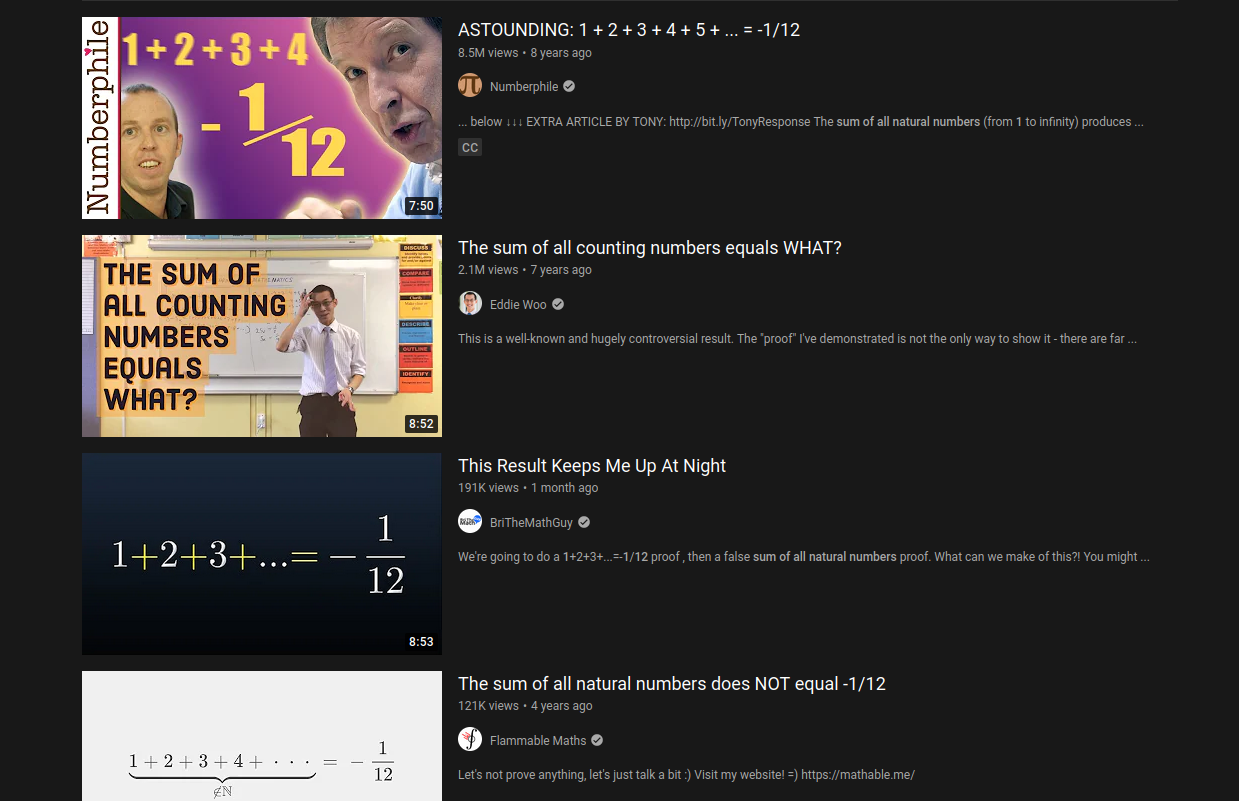
\includegraphics[width=0.7\textwidth]{youtube_screenshot.png}
        \end{center}
    \end{frame}
    \begin{frame}
        \frametitle{Riemannsche Zeta Funktion}
        \begin{equation*}
            \zeta(s)
            =
            \sum_{n=1}^{\infty}
            \frac{1}{n^s}
        \end{equation*}
        \pause
        \begin{equation*}
            \zeta(-1)
            =
            \sum_{n=1}^{\infty}
            \frac{1}{n^{-1}}
            =
            \sum_{n=1}^{\infty} n
        \end{equation*}
    \end{frame}
    \begin{frame}
        \frametitle{Originaler Definitionsbereich}
        Wir kennen die divergierende harmonische Reihe
        \begin{equation*}
            \zeta(1)
            =
            \sum_{n=1}^{\infty}
            \frac{1}{n}
            \rightarrow
            \infty,
        \end{equation*}
        und somit ist $\Re(s) > 1$.
    \end{frame}

    \section{Analytische Fortsetzung}
    \begin{frame}
        \frametitle{Plan für die Analytische Fortsetzung von $\zeta(s)$}
        \begin{center}
            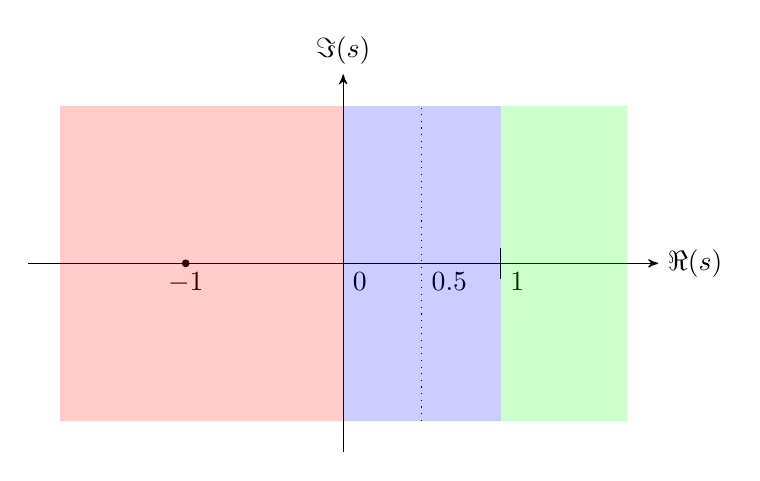
\begin{tikzpicture}[>=stealth', auto, node distance=0.9cm, scale=2,
    dot/.style={fill, circle, inner sep=0, minimum size=0.1cm}]

    \draw[->] (-2,0) -- (-1,0) node[dot]{} node[anchor=north]{$-1$} -- (0,0) node[anchor=north west]{$0$} -- (0.5,0) node[anchor=north west]{$0.5$}-- (1,0) node[anchor=north west]{$1$} -- (2,0) node[anchor=west]{$\Re(s)$};

    \draw[->] (0,-1.2) -- (0,1.2) node[anchor=south]{$\Im(s)$};
    \begin{scope}[yscale=0.1]
        \draw[] (1,-1) -- (1,1);
    \end{scope}
    \draw[dotted] (0.5,-1) -- (0.5,1);

    \begin{scope}[]
        \fill[opacity=0.2, red] (-1.8,1) rectangle (0, -1);
        \fill[opacity=0.2, blue] (0,1) rectangle (1, -1);
        \fill[opacity=0.2, green] (1,1) rectangle (1.8, -1);
    \end{scope}

\end{tikzpicture}

        \end{center}
    \end{frame}
    \begin{frame}
        \frametitle{Fortsetzung auf $\Re(s) > 0$}
        Dirichletsche Etafunktion ist
        \begin{equation*}\label{zeta:equation:eta}
            \eta(s)
            =
            \sum_{n=1}^{\infty}
            \frac{(-1)^{n-1}}{n^s},
        \end{equation*}
        und konvergiert im Bereich $\Re(s) > 0$.
    \end{frame}
    \begin{frame}
        \frametitle{Fortsetzung auf $\Re(s) > 0$}
        \begin{align}
            \zeta(s)
            &=
            \RD{
            \sum_{n=1}^{\infty}
            \frac{1}{n^s} \label{zeta:align1}
            }
            \\
            \frac{1}{2^{s-1}}
            \zeta(s)
            &=
            \BL{
            \sum_{n=1}^{\infty}
            \frac{2}{(2n)^s} \label{zeta:align2}
            }
        \end{align}
        \pause
        \eqref{zeta:align1} - \eqref{zeta:align2}:
        \begin{align*}
            \left(1 - \frac{1}{2^{s-1}} \right)
            \zeta(s)
            &=
            \RD{\frac{1}{1^s}}
            \underbrace{-\BL{\frac{2}{2^s}} + \RD{\frac{1}{2^s}}}_{-\frac{1}{2^s}}
            + \RD{\frac{1}{3^s}}
            \underbrace{-\BL{\frac{2}{4^s}} + \RD{\frac{1}{4^s}}}_{-\frac{1}{4^s}}
            \ldots
            \\
            &= \eta(s)
        \end{align*}
    \end{frame}
    \begin{frame}
        \frametitle{Fortsetzung auf $\Re(s) > 0$}
        Somit haben wir die Fortsetzung gefunden als
        \begin{equation} \label{zeta:equation:fortsetzung1}
            \zeta(s)
            :=
            \left(1 - \frac{1}{2^{s-1}} \right)^{-1} \eta(s).
        \end{equation}
    \end{frame}
    \begin{frame}
        \frametitle{Spiegelungseigenschaft für $\Re(s) < 0$}
        \begin{equation*}\label{zeta:equation:functional}
            \frac{\Gamma \left( \frac{s}{2} \right)}{\pi^{\frac{s}{2}}}
            \zeta(s)
            =
            \frac{\Gamma \left( \frac{1-s}{2} \right)}{\pi^{\frac{1-s}{2}}}
            \zeta(1-s).
        \end{equation*}
    \end{frame}
    %TODO maybe explain gamma-fct

    \section{Euler Produkt und Primzahlen}
    \begin{frame}
        \frametitle{Wieso ist die Zeta Funktion so bekannt?}
        \begin{itemize}
            \item Interessante Funktionswerte z.B. $\zeta(2) = \frac{\pi^2}{6}$
            \item Primzahlenverteilung (Riemannhypothese)
            \item Forschungsgebiet der analytischen Zahlentheorie seit dem 18. Jahrhundert
            \item ...
        \end{itemize}
    \end{frame}
    \begin{frame}
        \frametitle{Euler Produkt: Verbindung von Zeta und Primzahlen}
        \begin{equation*}
            \zeta(s)
            =
            \sum_{n=1}^\infty
            \frac{1}{n^s}
            =
            \prod_{p \in P}
            \frac{1}{1-p^{-s}}
        \end{equation*}
        \pause
        Geometrische Reihe
        \begin{equation*}
            \prod_{p \in P}
            \frac{1}{1-p^{-s}}
            =
            \prod_{p \in P}
            \left(
            1
            +
            \frac{1}{p^s}
            +
            \frac{1}{p^{2s}}
            +
            \frac{1}{p^{3s}}
            +
            \ldots
            \right)
        \end{equation*}
        \pause
        Erste Terme ausmultiplizieren
        \begin{align*}
            \left(
            1
            +
            \RD{\frac{1}{2^s}}
            +
            \GN{\frac{1}{2^{2s}}}
            +
            \frac{1}{2^{3s}}
            +
            \ldots
            \right)
            \left(
            1
            +
            \BL{\frac{1}{3^s}}
            +
            \frac{1}{3^{2s}}
            +
            \frac{1}{3^{3s}}
            +
            \ldots
            \right)
            \left(
            1
            +
            \YE{\frac{1}{5^s}}
            +
            \frac{1}{5^{2s}}
            +
            \frac{1}{5^{3s}}
            +
            \ldots
            \right)
            \ldots
            \\
            =
            1
            +
            \RD{\frac{1}{2^s}}
            +
            \BL{\frac{1}{3^s}}
            +
            \GN{\frac{1}{4^s}}
            +
            \YE{\frac{1}{5^s}}
            +
            \ldots
        \end{align*}
    \end{frame}
    \begin{frame}
        \frametitle{Primzahlfunktion}
        \begin{center}
           \scalebox{0.5}{%% Creator: Matplotlib, PGF backend
%%
%% To include the figure in your LaTeX document, write
%%   \input{<filename>.pgf}
%%
%% Make sure the required packages are loaded in your preamble
%%   \usepackage{pgf}
%%
%% and, on pdftex
%%   \usepackage[utf8]{inputenc}\DeclareUnicodeCharacter{2212}{-}
%%
%% or, on luatex and xetex
%%   \usepackage{unicode-math}
%%
%% Figures using additional raster images can only be included by \input if
%% they are in the same directory as the main LaTeX file. For loading figures
%% from other directories you can use the `import` package
%%   \usepackage{import}
%%
%% and then include the figures with
%%   \import{<path to file>}{<filename>.pgf}
%%
%% Matplotlib used the following preamble
%%
\begingroup%
\makeatletter%
\begin{pgfpicture}%
\pgfpathrectangle{\pgfpointorigin}{\pgfqpoint{6.400000in}{4.800000in}}%
\pgfusepath{use as bounding box, clip}%
\begin{pgfscope}%
\pgfsetbuttcap%
\pgfsetmiterjoin%
\definecolor{currentfill}{rgb}{1.000000,1.000000,1.000000}%
\pgfsetfillcolor{currentfill}%
\pgfsetlinewidth{0.000000pt}%
\definecolor{currentstroke}{rgb}{1.000000,1.000000,1.000000}%
\pgfsetstrokecolor{currentstroke}%
\pgfsetdash{}{0pt}%
\pgfpathmoveto{\pgfqpoint{0.000000in}{0.000000in}}%
\pgfpathlineto{\pgfqpoint{6.400000in}{0.000000in}}%
\pgfpathlineto{\pgfqpoint{6.400000in}{4.800000in}}%
\pgfpathlineto{\pgfqpoint{0.000000in}{4.800000in}}%
\pgfpathclose%
\pgfusepath{fill}%
\end{pgfscope}%
\begin{pgfscope}%
\pgfsetbuttcap%
\pgfsetmiterjoin%
\definecolor{currentfill}{rgb}{1.000000,1.000000,1.000000}%
\pgfsetfillcolor{currentfill}%
\pgfsetlinewidth{0.000000pt}%
\definecolor{currentstroke}{rgb}{0.000000,0.000000,0.000000}%
\pgfsetstrokecolor{currentstroke}%
\pgfsetstrokeopacity{0.000000}%
\pgfsetdash{}{0pt}%
\pgfpathmoveto{\pgfqpoint{0.800000in}{0.528000in}}%
\pgfpathlineto{\pgfqpoint{5.760000in}{0.528000in}}%
\pgfpathlineto{\pgfqpoint{5.760000in}{4.224000in}}%
\pgfpathlineto{\pgfqpoint{0.800000in}{4.224000in}}%
\pgfpathclose%
\pgfusepath{fill}%
\end{pgfscope}%
\begin{pgfscope}%
\pgfsetbuttcap%
\pgfsetroundjoin%
\definecolor{currentfill}{rgb}{0.000000,0.000000,0.000000}%
\pgfsetfillcolor{currentfill}%
\pgfsetlinewidth{0.803000pt}%
\definecolor{currentstroke}{rgb}{0.000000,0.000000,0.000000}%
\pgfsetstrokecolor{currentstroke}%
\pgfsetdash{}{0pt}%
\pgfsys@defobject{currentmarker}{\pgfqpoint{0.000000in}{-0.048611in}}{\pgfqpoint{0.000000in}{0.000000in}}{%
\pgfpathmoveto{\pgfqpoint{0.000000in}{0.000000in}}%
\pgfpathlineto{\pgfqpoint{0.000000in}{-0.048611in}}%
\pgfusepath{stroke,fill}%
}%
\begin{pgfscope}%
\pgfsys@transformshift{1.025455in}{0.528000in}%
\pgfsys@useobject{currentmarker}{}%
\end{pgfscope}%
\end{pgfscope}%
\begin{pgfscope}%
\definecolor{textcolor}{rgb}{0.000000,0.000000,0.000000}%
\pgfsetstrokecolor{textcolor}%
\pgfsetfillcolor{textcolor}%
\pgftext[x=1.025455in,y=0.430778in,,top]{\color{textcolor}\sffamily\fontsize{10.000000}{12.000000}\selectfont 0}%
\end{pgfscope}%
\begin{pgfscope}%
\pgfsetbuttcap%
\pgfsetroundjoin%
\definecolor{currentfill}{rgb}{0.000000,0.000000,0.000000}%
\pgfsetfillcolor{currentfill}%
\pgfsetlinewidth{0.803000pt}%
\definecolor{currentstroke}{rgb}{0.000000,0.000000,0.000000}%
\pgfsetstrokecolor{currentstroke}%
\pgfsetdash{}{0pt}%
\pgfsys@defobject{currentmarker}{\pgfqpoint{0.000000in}{-0.048611in}}{\pgfqpoint{0.000000in}{0.000000in}}{%
\pgfpathmoveto{\pgfqpoint{0.000000in}{0.000000in}}%
\pgfpathlineto{\pgfqpoint{0.000000in}{-0.048611in}}%
\pgfusepath{stroke,fill}%
}%
\begin{pgfscope}%
\pgfsys@transformshift{1.776970in}{0.528000in}%
\pgfsys@useobject{currentmarker}{}%
\end{pgfscope}%
\end{pgfscope}%
\begin{pgfscope}%
\definecolor{textcolor}{rgb}{0.000000,0.000000,0.000000}%
\pgfsetstrokecolor{textcolor}%
\pgfsetfillcolor{textcolor}%
\pgftext[x=1.776970in,y=0.430778in,,top]{\color{textcolor}\sffamily\fontsize{10.000000}{12.000000}\selectfont 5}%
\end{pgfscope}%
\begin{pgfscope}%
\pgfsetbuttcap%
\pgfsetroundjoin%
\definecolor{currentfill}{rgb}{0.000000,0.000000,0.000000}%
\pgfsetfillcolor{currentfill}%
\pgfsetlinewidth{0.803000pt}%
\definecolor{currentstroke}{rgb}{0.000000,0.000000,0.000000}%
\pgfsetstrokecolor{currentstroke}%
\pgfsetdash{}{0pt}%
\pgfsys@defobject{currentmarker}{\pgfqpoint{0.000000in}{-0.048611in}}{\pgfqpoint{0.000000in}{0.000000in}}{%
\pgfpathmoveto{\pgfqpoint{0.000000in}{0.000000in}}%
\pgfpathlineto{\pgfqpoint{0.000000in}{-0.048611in}}%
\pgfusepath{stroke,fill}%
}%
\begin{pgfscope}%
\pgfsys@transformshift{2.528485in}{0.528000in}%
\pgfsys@useobject{currentmarker}{}%
\end{pgfscope}%
\end{pgfscope}%
\begin{pgfscope}%
\definecolor{textcolor}{rgb}{0.000000,0.000000,0.000000}%
\pgfsetstrokecolor{textcolor}%
\pgfsetfillcolor{textcolor}%
\pgftext[x=2.528485in,y=0.430778in,,top]{\color{textcolor}\sffamily\fontsize{10.000000}{12.000000}\selectfont 10}%
\end{pgfscope}%
\begin{pgfscope}%
\pgfsetbuttcap%
\pgfsetroundjoin%
\definecolor{currentfill}{rgb}{0.000000,0.000000,0.000000}%
\pgfsetfillcolor{currentfill}%
\pgfsetlinewidth{0.803000pt}%
\definecolor{currentstroke}{rgb}{0.000000,0.000000,0.000000}%
\pgfsetstrokecolor{currentstroke}%
\pgfsetdash{}{0pt}%
\pgfsys@defobject{currentmarker}{\pgfqpoint{0.000000in}{-0.048611in}}{\pgfqpoint{0.000000in}{0.000000in}}{%
\pgfpathmoveto{\pgfqpoint{0.000000in}{0.000000in}}%
\pgfpathlineto{\pgfqpoint{0.000000in}{-0.048611in}}%
\pgfusepath{stroke,fill}%
}%
\begin{pgfscope}%
\pgfsys@transformshift{3.280000in}{0.528000in}%
\pgfsys@useobject{currentmarker}{}%
\end{pgfscope}%
\end{pgfscope}%
\begin{pgfscope}%
\definecolor{textcolor}{rgb}{0.000000,0.000000,0.000000}%
\pgfsetstrokecolor{textcolor}%
\pgfsetfillcolor{textcolor}%
\pgftext[x=3.280000in,y=0.430778in,,top]{\color{textcolor}\sffamily\fontsize{10.000000}{12.000000}\selectfont 15}%
\end{pgfscope}%
\begin{pgfscope}%
\pgfsetbuttcap%
\pgfsetroundjoin%
\definecolor{currentfill}{rgb}{0.000000,0.000000,0.000000}%
\pgfsetfillcolor{currentfill}%
\pgfsetlinewidth{0.803000pt}%
\definecolor{currentstroke}{rgb}{0.000000,0.000000,0.000000}%
\pgfsetstrokecolor{currentstroke}%
\pgfsetdash{}{0pt}%
\pgfsys@defobject{currentmarker}{\pgfqpoint{0.000000in}{-0.048611in}}{\pgfqpoint{0.000000in}{0.000000in}}{%
\pgfpathmoveto{\pgfqpoint{0.000000in}{0.000000in}}%
\pgfpathlineto{\pgfqpoint{0.000000in}{-0.048611in}}%
\pgfusepath{stroke,fill}%
}%
\begin{pgfscope}%
\pgfsys@transformshift{4.031515in}{0.528000in}%
\pgfsys@useobject{currentmarker}{}%
\end{pgfscope}%
\end{pgfscope}%
\begin{pgfscope}%
\definecolor{textcolor}{rgb}{0.000000,0.000000,0.000000}%
\pgfsetstrokecolor{textcolor}%
\pgfsetfillcolor{textcolor}%
\pgftext[x=4.031515in,y=0.430778in,,top]{\color{textcolor}\sffamily\fontsize{10.000000}{12.000000}\selectfont 20}%
\end{pgfscope}%
\begin{pgfscope}%
\pgfsetbuttcap%
\pgfsetroundjoin%
\definecolor{currentfill}{rgb}{0.000000,0.000000,0.000000}%
\pgfsetfillcolor{currentfill}%
\pgfsetlinewidth{0.803000pt}%
\definecolor{currentstroke}{rgb}{0.000000,0.000000,0.000000}%
\pgfsetstrokecolor{currentstroke}%
\pgfsetdash{}{0pt}%
\pgfsys@defobject{currentmarker}{\pgfqpoint{0.000000in}{-0.048611in}}{\pgfqpoint{0.000000in}{0.000000in}}{%
\pgfpathmoveto{\pgfqpoint{0.000000in}{0.000000in}}%
\pgfpathlineto{\pgfqpoint{0.000000in}{-0.048611in}}%
\pgfusepath{stroke,fill}%
}%
\begin{pgfscope}%
\pgfsys@transformshift{4.783030in}{0.528000in}%
\pgfsys@useobject{currentmarker}{}%
\end{pgfscope}%
\end{pgfscope}%
\begin{pgfscope}%
\definecolor{textcolor}{rgb}{0.000000,0.000000,0.000000}%
\pgfsetstrokecolor{textcolor}%
\pgfsetfillcolor{textcolor}%
\pgftext[x=4.783030in,y=0.430778in,,top]{\color{textcolor}\sffamily\fontsize{10.000000}{12.000000}\selectfont 25}%
\end{pgfscope}%
\begin{pgfscope}%
\pgfsetbuttcap%
\pgfsetroundjoin%
\definecolor{currentfill}{rgb}{0.000000,0.000000,0.000000}%
\pgfsetfillcolor{currentfill}%
\pgfsetlinewidth{0.803000pt}%
\definecolor{currentstroke}{rgb}{0.000000,0.000000,0.000000}%
\pgfsetstrokecolor{currentstroke}%
\pgfsetdash{}{0pt}%
\pgfsys@defobject{currentmarker}{\pgfqpoint{0.000000in}{-0.048611in}}{\pgfqpoint{0.000000in}{0.000000in}}{%
\pgfpathmoveto{\pgfqpoint{0.000000in}{0.000000in}}%
\pgfpathlineto{\pgfqpoint{0.000000in}{-0.048611in}}%
\pgfusepath{stroke,fill}%
}%
\begin{pgfscope}%
\pgfsys@transformshift{5.534545in}{0.528000in}%
\pgfsys@useobject{currentmarker}{}%
\end{pgfscope}%
\end{pgfscope}%
\begin{pgfscope}%
\definecolor{textcolor}{rgb}{0.000000,0.000000,0.000000}%
\pgfsetstrokecolor{textcolor}%
\pgfsetfillcolor{textcolor}%
\pgftext[x=5.534545in,y=0.430778in,,top]{\color{textcolor}\sffamily\fontsize{10.000000}{12.000000}\selectfont 30}%
\end{pgfscope}%
\begin{pgfscope}%
\pgfsetbuttcap%
\pgfsetroundjoin%
\definecolor{currentfill}{rgb}{0.000000,0.000000,0.000000}%
\pgfsetfillcolor{currentfill}%
\pgfsetlinewidth{0.803000pt}%
\definecolor{currentstroke}{rgb}{0.000000,0.000000,0.000000}%
\pgfsetstrokecolor{currentstroke}%
\pgfsetdash{}{0pt}%
\pgfsys@defobject{currentmarker}{\pgfqpoint{-0.048611in}{0.000000in}}{\pgfqpoint{-0.000000in}{0.000000in}}{%
\pgfpathmoveto{\pgfqpoint{-0.000000in}{0.000000in}}%
\pgfpathlineto{\pgfqpoint{-0.048611in}{0.000000in}}%
\pgfusepath{stroke,fill}%
}%
\begin{pgfscope}%
\pgfsys@transformshift{0.800000in}{0.696000in}%
\pgfsys@useobject{currentmarker}{}%
\end{pgfscope}%
\end{pgfscope}%
\begin{pgfscope}%
\definecolor{textcolor}{rgb}{0.000000,0.000000,0.000000}%
\pgfsetstrokecolor{textcolor}%
\pgfsetfillcolor{textcolor}%
\pgftext[x=0.633333in, y=0.647775in, left, base]{\color{textcolor}\sffamily\fontsize{10.000000}{12.000000}\selectfont 0}%
\end{pgfscope}%
\begin{pgfscope}%
\pgfsetbuttcap%
\pgfsetroundjoin%
\definecolor{currentfill}{rgb}{0.000000,0.000000,0.000000}%
\pgfsetfillcolor{currentfill}%
\pgfsetlinewidth{0.803000pt}%
\definecolor{currentstroke}{rgb}{0.000000,0.000000,0.000000}%
\pgfsetstrokecolor{currentstroke}%
\pgfsetdash{}{0pt}%
\pgfsys@defobject{currentmarker}{\pgfqpoint{-0.048611in}{0.000000in}}{\pgfqpoint{-0.000000in}{0.000000in}}{%
\pgfpathmoveto{\pgfqpoint{-0.000000in}{0.000000in}}%
\pgfpathlineto{\pgfqpoint{-0.048611in}{0.000000in}}%
\pgfusepath{stroke,fill}%
}%
\begin{pgfscope}%
\pgfsys@transformshift{0.800000in}{1.368000in}%
\pgfsys@useobject{currentmarker}{}%
\end{pgfscope}%
\end{pgfscope}%
\begin{pgfscope}%
\definecolor{textcolor}{rgb}{0.000000,0.000000,0.000000}%
\pgfsetstrokecolor{textcolor}%
\pgfsetfillcolor{textcolor}%
\pgftext[x=0.633333in, y=1.319775in, left, base]{\color{textcolor}\sffamily\fontsize{10.000000}{12.000000}\selectfont 2}%
\end{pgfscope}%
\begin{pgfscope}%
\pgfsetbuttcap%
\pgfsetroundjoin%
\definecolor{currentfill}{rgb}{0.000000,0.000000,0.000000}%
\pgfsetfillcolor{currentfill}%
\pgfsetlinewidth{0.803000pt}%
\definecolor{currentstroke}{rgb}{0.000000,0.000000,0.000000}%
\pgfsetstrokecolor{currentstroke}%
\pgfsetdash{}{0pt}%
\pgfsys@defobject{currentmarker}{\pgfqpoint{-0.048611in}{0.000000in}}{\pgfqpoint{-0.000000in}{0.000000in}}{%
\pgfpathmoveto{\pgfqpoint{-0.000000in}{0.000000in}}%
\pgfpathlineto{\pgfqpoint{-0.048611in}{0.000000in}}%
\pgfusepath{stroke,fill}%
}%
\begin{pgfscope}%
\pgfsys@transformshift{0.800000in}{2.040000in}%
\pgfsys@useobject{currentmarker}{}%
\end{pgfscope}%
\end{pgfscope}%
\begin{pgfscope}%
\definecolor{textcolor}{rgb}{0.000000,0.000000,0.000000}%
\pgfsetstrokecolor{textcolor}%
\pgfsetfillcolor{textcolor}%
\pgftext[x=0.633333in, y=1.991775in, left, base]{\color{textcolor}\sffamily\fontsize{10.000000}{12.000000}\selectfont 4}%
\end{pgfscope}%
\begin{pgfscope}%
\pgfsetbuttcap%
\pgfsetroundjoin%
\definecolor{currentfill}{rgb}{0.000000,0.000000,0.000000}%
\pgfsetfillcolor{currentfill}%
\pgfsetlinewidth{0.803000pt}%
\definecolor{currentstroke}{rgb}{0.000000,0.000000,0.000000}%
\pgfsetstrokecolor{currentstroke}%
\pgfsetdash{}{0pt}%
\pgfsys@defobject{currentmarker}{\pgfqpoint{-0.048611in}{0.000000in}}{\pgfqpoint{-0.000000in}{0.000000in}}{%
\pgfpathmoveto{\pgfqpoint{-0.000000in}{0.000000in}}%
\pgfpathlineto{\pgfqpoint{-0.048611in}{0.000000in}}%
\pgfusepath{stroke,fill}%
}%
\begin{pgfscope}%
\pgfsys@transformshift{0.800000in}{2.712000in}%
\pgfsys@useobject{currentmarker}{}%
\end{pgfscope}%
\end{pgfscope}%
\begin{pgfscope}%
\definecolor{textcolor}{rgb}{0.000000,0.000000,0.000000}%
\pgfsetstrokecolor{textcolor}%
\pgfsetfillcolor{textcolor}%
\pgftext[x=0.633333in, y=2.663775in, left, base]{\color{textcolor}\sffamily\fontsize{10.000000}{12.000000}\selectfont 6}%
\end{pgfscope}%
\begin{pgfscope}%
\pgfsetbuttcap%
\pgfsetroundjoin%
\definecolor{currentfill}{rgb}{0.000000,0.000000,0.000000}%
\pgfsetfillcolor{currentfill}%
\pgfsetlinewidth{0.803000pt}%
\definecolor{currentstroke}{rgb}{0.000000,0.000000,0.000000}%
\pgfsetstrokecolor{currentstroke}%
\pgfsetdash{}{0pt}%
\pgfsys@defobject{currentmarker}{\pgfqpoint{-0.048611in}{0.000000in}}{\pgfqpoint{-0.000000in}{0.000000in}}{%
\pgfpathmoveto{\pgfqpoint{-0.000000in}{0.000000in}}%
\pgfpathlineto{\pgfqpoint{-0.048611in}{0.000000in}}%
\pgfusepath{stroke,fill}%
}%
\begin{pgfscope}%
\pgfsys@transformshift{0.800000in}{3.384000in}%
\pgfsys@useobject{currentmarker}{}%
\end{pgfscope}%
\end{pgfscope}%
\begin{pgfscope}%
\definecolor{textcolor}{rgb}{0.000000,0.000000,0.000000}%
\pgfsetstrokecolor{textcolor}%
\pgfsetfillcolor{textcolor}%
\pgftext[x=0.633333in, y=3.335775in, left, base]{\color{textcolor}\sffamily\fontsize{10.000000}{12.000000}\selectfont 8}%
\end{pgfscope}%
\begin{pgfscope}%
\pgfsetbuttcap%
\pgfsetroundjoin%
\definecolor{currentfill}{rgb}{0.000000,0.000000,0.000000}%
\pgfsetfillcolor{currentfill}%
\pgfsetlinewidth{0.803000pt}%
\definecolor{currentstroke}{rgb}{0.000000,0.000000,0.000000}%
\pgfsetstrokecolor{currentstroke}%
\pgfsetdash{}{0pt}%
\pgfsys@defobject{currentmarker}{\pgfqpoint{-0.048611in}{0.000000in}}{\pgfqpoint{-0.000000in}{0.000000in}}{%
\pgfpathmoveto{\pgfqpoint{-0.000000in}{0.000000in}}%
\pgfpathlineto{\pgfqpoint{-0.048611in}{0.000000in}}%
\pgfusepath{stroke,fill}%
}%
\begin{pgfscope}%
\pgfsys@transformshift{0.800000in}{4.056000in}%
\pgfsys@useobject{currentmarker}{}%
\end{pgfscope}%
\end{pgfscope}%
\begin{pgfscope}%
\definecolor{textcolor}{rgb}{0.000000,0.000000,0.000000}%
\pgfsetstrokecolor{textcolor}%
\pgfsetfillcolor{textcolor}%
\pgftext[x=0.563888in, y=4.007775in, left, base]{\color{textcolor}\sffamily\fontsize{10.000000}{12.000000}\selectfont 10}%
\end{pgfscope}%
\begin{pgfscope}%
\pgfpathrectangle{\pgfqpoint{0.800000in}{0.528000in}}{\pgfqpoint{4.960000in}{3.696000in}}%
\pgfusepath{clip}%
\pgfsetrectcap%
\pgfsetroundjoin%
\pgfsetlinewidth{1.505625pt}%
\definecolor{currentstroke}{rgb}{0.121569,0.466667,0.705882}%
\pgfsetstrokecolor{currentstroke}%
\pgfsetdash{}{0pt}%
\pgfpathmoveto{\pgfqpoint{1.025455in}{0.696000in}}%
\pgfpathlineto{\pgfqpoint{1.175758in}{0.696000in}}%
\pgfpathlineto{\pgfqpoint{1.175758in}{0.696000in}}%
\pgfpathlineto{\pgfqpoint{1.326061in}{0.696000in}}%
\pgfpathlineto{\pgfqpoint{1.326061in}{1.032000in}}%
\pgfpathlineto{\pgfqpoint{1.476364in}{1.032000in}}%
\pgfpathlineto{\pgfqpoint{1.476364in}{1.368000in}}%
\pgfpathlineto{\pgfqpoint{1.626667in}{1.368000in}}%
\pgfpathlineto{\pgfqpoint{1.626667in}{1.368000in}}%
\pgfpathlineto{\pgfqpoint{1.776970in}{1.368000in}}%
\pgfpathlineto{\pgfqpoint{1.776970in}{1.704000in}}%
\pgfpathlineto{\pgfqpoint{1.927273in}{1.704000in}}%
\pgfpathlineto{\pgfqpoint{1.927273in}{1.704000in}}%
\pgfpathlineto{\pgfqpoint{2.077576in}{1.704000in}}%
\pgfpathlineto{\pgfqpoint{2.077576in}{2.040000in}}%
\pgfpathlineto{\pgfqpoint{2.227879in}{2.040000in}}%
\pgfpathlineto{\pgfqpoint{2.227879in}{2.040000in}}%
\pgfpathlineto{\pgfqpoint{2.378182in}{2.040000in}}%
\pgfpathlineto{\pgfqpoint{2.378182in}{2.040000in}}%
\pgfpathlineto{\pgfqpoint{2.528485in}{2.040000in}}%
\pgfpathlineto{\pgfqpoint{2.528485in}{2.040000in}}%
\pgfpathlineto{\pgfqpoint{2.678788in}{2.040000in}}%
\pgfpathlineto{\pgfqpoint{2.678788in}{2.376000in}}%
\pgfpathlineto{\pgfqpoint{2.829091in}{2.376000in}}%
\pgfpathlineto{\pgfqpoint{2.829091in}{2.376000in}}%
\pgfpathlineto{\pgfqpoint{2.979394in}{2.376000in}}%
\pgfpathlineto{\pgfqpoint{2.979394in}{2.712000in}}%
\pgfpathlineto{\pgfqpoint{3.129697in}{2.712000in}}%
\pgfpathlineto{\pgfqpoint{3.129697in}{2.712000in}}%
\pgfpathlineto{\pgfqpoint{3.280000in}{2.712000in}}%
\pgfpathlineto{\pgfqpoint{3.280000in}{2.712000in}}%
\pgfpathlineto{\pgfqpoint{3.430303in}{2.712000in}}%
\pgfpathlineto{\pgfqpoint{3.430303in}{2.712000in}}%
\pgfpathlineto{\pgfqpoint{3.580606in}{2.712000in}}%
\pgfpathlineto{\pgfqpoint{3.580606in}{3.048000in}}%
\pgfpathlineto{\pgfqpoint{3.730909in}{3.048000in}}%
\pgfpathlineto{\pgfqpoint{3.730909in}{3.048000in}}%
\pgfpathlineto{\pgfqpoint{3.881212in}{3.048000in}}%
\pgfpathlineto{\pgfqpoint{3.881212in}{3.384000in}}%
\pgfpathlineto{\pgfqpoint{4.031515in}{3.384000in}}%
\pgfpathlineto{\pgfqpoint{4.031515in}{3.384000in}}%
\pgfpathlineto{\pgfqpoint{4.181818in}{3.384000in}}%
\pgfpathlineto{\pgfqpoint{4.181818in}{3.384000in}}%
\pgfpathlineto{\pgfqpoint{4.332121in}{3.384000in}}%
\pgfpathlineto{\pgfqpoint{4.332121in}{3.384000in}}%
\pgfpathlineto{\pgfqpoint{4.482424in}{3.384000in}}%
\pgfpathlineto{\pgfqpoint{4.482424in}{3.720000in}}%
\pgfpathlineto{\pgfqpoint{4.632727in}{3.720000in}}%
\pgfpathlineto{\pgfqpoint{4.632727in}{3.720000in}}%
\pgfpathlineto{\pgfqpoint{4.783030in}{3.720000in}}%
\pgfpathlineto{\pgfqpoint{4.783030in}{3.720000in}}%
\pgfpathlineto{\pgfqpoint{4.933333in}{3.720000in}}%
\pgfpathlineto{\pgfqpoint{4.933333in}{3.720000in}}%
\pgfpathlineto{\pgfqpoint{5.083636in}{3.720000in}}%
\pgfpathlineto{\pgfqpoint{5.083636in}{3.720000in}}%
\pgfpathlineto{\pgfqpoint{5.233939in}{3.720000in}}%
\pgfpathlineto{\pgfqpoint{5.233939in}{3.720000in}}%
\pgfpathlineto{\pgfqpoint{5.384242in}{3.720000in}}%
\pgfpathlineto{\pgfqpoint{5.384242in}{4.056000in}}%
\pgfpathlineto{\pgfqpoint{5.534545in}{4.056000in}}%
\pgfusepath{stroke}%
\end{pgfscope}%
\begin{pgfscope}%
\pgfsetrectcap%
\pgfsetmiterjoin%
\pgfsetlinewidth{0.803000pt}%
\definecolor{currentstroke}{rgb}{0.000000,0.000000,0.000000}%
\pgfsetstrokecolor{currentstroke}%
\pgfsetdash{}{0pt}%
\pgfpathmoveto{\pgfqpoint{0.800000in}{0.528000in}}%
\pgfpathlineto{\pgfqpoint{0.800000in}{4.224000in}}%
\pgfusepath{stroke}%
\end{pgfscope}%
\begin{pgfscope}%
\pgfsetrectcap%
\pgfsetmiterjoin%
\pgfsetlinewidth{0.803000pt}%
\definecolor{currentstroke}{rgb}{0.000000,0.000000,0.000000}%
\pgfsetstrokecolor{currentstroke}%
\pgfsetdash{}{0pt}%
\pgfpathmoveto{\pgfqpoint{5.760000in}{0.528000in}}%
\pgfpathlineto{\pgfqpoint{5.760000in}{4.224000in}}%
\pgfusepath{stroke}%
\end{pgfscope}%
\begin{pgfscope}%
\pgfsetrectcap%
\pgfsetmiterjoin%
\pgfsetlinewidth{0.803000pt}%
\definecolor{currentstroke}{rgb}{0.000000,0.000000,0.000000}%
\pgfsetstrokecolor{currentstroke}%
\pgfsetdash{}{0pt}%
\pgfpathmoveto{\pgfqpoint{0.800000in}{0.528000in}}%
\pgfpathlineto{\pgfqpoint{5.760000in}{0.528000in}}%
\pgfusepath{stroke}%
\end{pgfscope}%
\begin{pgfscope}%
\pgfsetrectcap%
\pgfsetmiterjoin%
\pgfsetlinewidth{0.803000pt}%
\definecolor{currentstroke}{rgb}{0.000000,0.000000,0.000000}%
\pgfsetstrokecolor{currentstroke}%
\pgfsetdash{}{0pt}%
\pgfpathmoveto{\pgfqpoint{0.800000in}{4.224000in}}%
\pgfpathlineto{\pgfqpoint{5.760000in}{4.224000in}}%
\pgfusepath{stroke}%
\end{pgfscope}%
\end{pgfpicture}%
\makeatother%
\endgroup%
}
        \end{center}
    \end{frame}


    \section{Darstellungen}

    \begin{frame}
        \frametitle{Farbcodierung}
        \begin{center}
            \scalebox{0.6}{%% Creator: Matplotlib, PGF backend
%%
%% To include the figure in your LaTeX document, write
%%   \input{<filename>.pgf}
%%
%% Make sure the required packages are loaded in your preamble
%%   \usepackage{pgf}
%%
%% and, on pdftex
%%   \usepackage[utf8]{inputenc}\DeclareUnicodeCharacter{2212}{-}
%%
%% or, on luatex and xetex
%%   \usepackage{unicode-math}
%%
%% Figures using additional raster images can only be included by \input if
%% they are in the same directory as the main LaTeX file. For loading figures
%% from other directories you can use the `import` package
%%   \usepackage{import}
%%
%% and then include the figures with
%%   \import{<path to file>}{<filename>.pgf}
%%
%% Matplotlib used the following preamble
%%
\begingroup%
\makeatletter%
\begin{pgfpicture}%
\pgfpathrectangle{\pgfpointorigin}{\pgfqpoint{6.400000in}{4.800000in}}%
\pgfusepath{use as bounding box, clip}%
\begin{pgfscope}%
\pgfsetbuttcap%
\pgfsetmiterjoin%
\definecolor{currentfill}{rgb}{1.000000,1.000000,1.000000}%
\pgfsetfillcolor{currentfill}%
\pgfsetlinewidth{0.000000pt}%
\definecolor{currentstroke}{rgb}{1.000000,1.000000,1.000000}%
\pgfsetstrokecolor{currentstroke}%
\pgfsetdash{}{0pt}%
\pgfpathmoveto{\pgfqpoint{0.000000in}{0.000000in}}%
\pgfpathlineto{\pgfqpoint{6.400000in}{0.000000in}}%
\pgfpathlineto{\pgfqpoint{6.400000in}{4.800000in}}%
\pgfpathlineto{\pgfqpoint{0.000000in}{4.800000in}}%
\pgfpathclose%
\pgfusepath{fill}%
\end{pgfscope}%
\begin{pgfscope}%
\pgfsetbuttcap%
\pgfsetmiterjoin%
\definecolor{currentfill}{rgb}{1.000000,1.000000,1.000000}%
\pgfsetfillcolor{currentfill}%
\pgfsetlinewidth{0.000000pt}%
\definecolor{currentstroke}{rgb}{0.000000,0.000000,0.000000}%
\pgfsetstrokecolor{currentstroke}%
\pgfsetstrokeopacity{0.000000}%
\pgfsetdash{}{0pt}%
\pgfpathmoveto{\pgfqpoint{2.588156in}{0.528000in}}%
\pgfpathlineto{\pgfqpoint{3.971844in}{0.528000in}}%
\pgfpathlineto{\pgfqpoint{3.971844in}{4.224000in}}%
\pgfpathlineto{\pgfqpoint{2.588156in}{4.224000in}}%
\pgfpathclose%
\pgfusepath{fill}%
\end{pgfscope}%
\begin{pgfscope}%
\pgfpathrectangle{\pgfqpoint{2.588156in}{0.528000in}}{\pgfqpoint{1.383688in}{3.696000in}}%
\pgfusepath{clip}%
\pgfsys@transformshift{2.588156in}{0.528000in}%
\pgftext[left,bottom]{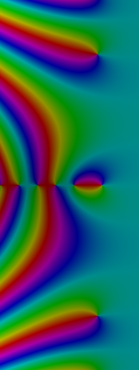
\includegraphics[interpolate=true,width=1.390000in,height=3.700000in]{zeta_color_plot-img0.png}}%
\end{pgfscope}%
\begin{pgfscope}%
\pgfsetbuttcap%
\pgfsetroundjoin%
\definecolor{currentfill}{rgb}{0.000000,0.000000,0.000000}%
\pgfsetfillcolor{currentfill}%
\pgfsetlinewidth{0.803000pt}%
\definecolor{currentstroke}{rgb}{0.000000,0.000000,0.000000}%
\pgfsetstrokecolor{currentstroke}%
\pgfsetdash{}{0pt}%
\pgfsys@defobject{currentmarker}{\pgfqpoint{0.000000in}{-0.048611in}}{\pgfqpoint{0.000000in}{0.000000in}}{%
\pgfpathmoveto{\pgfqpoint{0.000000in}{0.000000in}}%
\pgfpathlineto{\pgfqpoint{0.000000in}{-0.048611in}}%
\pgfusepath{stroke,fill}%
}%
\begin{pgfscope}%
\pgfsys@transformshift{2.588156in}{0.528000in}%
\pgfsys@useobject{currentmarker}{}%
\end{pgfscope}%
\end{pgfscope}%
\begin{pgfscope}%
\definecolor{textcolor}{rgb}{0.000000,0.000000,0.000000}%
\pgfsetstrokecolor{textcolor}%
\pgfsetfillcolor{textcolor}%
\pgftext[x=2.588156in,y=0.430778in,,top]{\color{textcolor}\rmfamily\fontsize{8.000000}{9.600000}\selectfont \(\displaystyle {-10}\)}%
\end{pgfscope}%
\begin{pgfscope}%
\pgfsetbuttcap%
\pgfsetroundjoin%
\definecolor{currentfill}{rgb}{0.000000,0.000000,0.000000}%
\pgfsetfillcolor{currentfill}%
\pgfsetlinewidth{0.803000pt}%
\definecolor{currentstroke}{rgb}{0.000000,0.000000,0.000000}%
\pgfsetstrokecolor{currentstroke}%
\pgfsetdash{}{0pt}%
\pgfsys@defobject{currentmarker}{\pgfqpoint{0.000000in}{-0.048611in}}{\pgfqpoint{0.000000in}{0.000000in}}{%
\pgfpathmoveto{\pgfqpoint{0.000000in}{0.000000in}}%
\pgfpathlineto{\pgfqpoint{0.000000in}{-0.048611in}}%
\pgfusepath{stroke,fill}%
}%
\begin{pgfscope}%
\pgfsys@transformshift{3.050619in}{0.528000in}%
\pgfsys@useobject{currentmarker}{}%
\end{pgfscope}%
\end{pgfscope}%
\begin{pgfscope}%
\definecolor{textcolor}{rgb}{0.000000,0.000000,0.000000}%
\pgfsetstrokecolor{textcolor}%
\pgfsetfillcolor{textcolor}%
\pgftext[x=3.050619in,y=0.430778in,,top]{\color{textcolor}\rmfamily\fontsize{8.000000}{9.600000}\selectfont \(\displaystyle {-5}\)}%
\end{pgfscope}%
\begin{pgfscope}%
\pgfsetbuttcap%
\pgfsetroundjoin%
\definecolor{currentfill}{rgb}{0.000000,0.000000,0.000000}%
\pgfsetfillcolor{currentfill}%
\pgfsetlinewidth{0.803000pt}%
\definecolor{currentstroke}{rgb}{0.000000,0.000000,0.000000}%
\pgfsetstrokecolor{currentstroke}%
\pgfsetdash{}{0pt}%
\pgfsys@defobject{currentmarker}{\pgfqpoint{0.000000in}{-0.048611in}}{\pgfqpoint{0.000000in}{0.000000in}}{%
\pgfpathmoveto{\pgfqpoint{0.000000in}{0.000000in}}%
\pgfpathlineto{\pgfqpoint{0.000000in}{-0.048611in}}%
\pgfusepath{stroke,fill}%
}%
\begin{pgfscope}%
\pgfsys@transformshift{3.513081in}{0.528000in}%
\pgfsys@useobject{currentmarker}{}%
\end{pgfscope}%
\end{pgfscope}%
\begin{pgfscope}%
\definecolor{textcolor}{rgb}{0.000000,0.000000,0.000000}%
\pgfsetstrokecolor{textcolor}%
\pgfsetfillcolor{textcolor}%
\pgftext[x=3.513081in,y=0.430778in,,top]{\color{textcolor}\rmfamily\fontsize{8.000000}{9.600000}\selectfont \(\displaystyle {0}\)}%
\end{pgfscope}%
\begin{pgfscope}%
\definecolor{textcolor}{rgb}{0.000000,0.000000,0.000000}%
\pgfsetstrokecolor{textcolor}%
\pgfsetfillcolor{textcolor}%
\pgftext[x=3.280000in,y=0.276457in,,top]{\color{textcolor}\rmfamily\fontsize{8.000000}{9.600000}\selectfont \(\displaystyle \Re\)}%
\end{pgfscope}%
\begin{pgfscope}%
\pgfsetbuttcap%
\pgfsetroundjoin%
\definecolor{currentfill}{rgb}{0.000000,0.000000,0.000000}%
\pgfsetfillcolor{currentfill}%
\pgfsetlinewidth{0.803000pt}%
\definecolor{currentstroke}{rgb}{0.000000,0.000000,0.000000}%
\pgfsetstrokecolor{currentstroke}%
\pgfsetdash{}{0pt}%
\pgfsys@defobject{currentmarker}{\pgfqpoint{-0.048611in}{0.000000in}}{\pgfqpoint{-0.000000in}{0.000000in}}{%
\pgfpathmoveto{\pgfqpoint{-0.000000in}{0.000000in}}%
\pgfpathlineto{\pgfqpoint{-0.048611in}{0.000000in}}%
\pgfusepath{stroke,fill}%
}%
\begin{pgfscope}%
\pgfsys@transformshift{2.588156in}{0.528000in}%
\pgfsys@useobject{currentmarker}{}%
\end{pgfscope}%
\end{pgfscope}%
\begin{pgfscope}%
\definecolor{textcolor}{rgb}{0.000000,0.000000,0.000000}%
\pgfsetstrokecolor{textcolor}%
\pgfsetfillcolor{textcolor}%
\pgftext[x=2.281054in, y=0.489420in, left, base]{\color{textcolor}\rmfamily\fontsize{8.000000}{9.600000}\selectfont \(\displaystyle {-20}\)}%
\end{pgfscope}%
\begin{pgfscope}%
\pgfsetbuttcap%
\pgfsetroundjoin%
\definecolor{currentfill}{rgb}{0.000000,0.000000,0.000000}%
\pgfsetfillcolor{currentfill}%
\pgfsetlinewidth{0.803000pt}%
\definecolor{currentstroke}{rgb}{0.000000,0.000000,0.000000}%
\pgfsetstrokecolor{currentstroke}%
\pgfsetdash{}{0pt}%
\pgfsys@defobject{currentmarker}{\pgfqpoint{-0.048611in}{0.000000in}}{\pgfqpoint{-0.000000in}{0.000000in}}{%
\pgfpathmoveto{\pgfqpoint{-0.000000in}{0.000000in}}%
\pgfpathlineto{\pgfqpoint{-0.048611in}{0.000000in}}%
\pgfusepath{stroke,fill}%
}%
\begin{pgfscope}%
\pgfsys@transformshift{2.588156in}{0.990462in}%
\pgfsys@useobject{currentmarker}{}%
\end{pgfscope}%
\end{pgfscope}%
\begin{pgfscope}%
\definecolor{textcolor}{rgb}{0.000000,0.000000,0.000000}%
\pgfsetstrokecolor{textcolor}%
\pgfsetfillcolor{textcolor}%
\pgftext[x=2.281054in, y=0.951882in, left, base]{\color{textcolor}\rmfamily\fontsize{8.000000}{9.600000}\selectfont \(\displaystyle {-15}\)}%
\end{pgfscope}%
\begin{pgfscope}%
\pgfsetbuttcap%
\pgfsetroundjoin%
\definecolor{currentfill}{rgb}{0.000000,0.000000,0.000000}%
\pgfsetfillcolor{currentfill}%
\pgfsetlinewidth{0.803000pt}%
\definecolor{currentstroke}{rgb}{0.000000,0.000000,0.000000}%
\pgfsetstrokecolor{currentstroke}%
\pgfsetdash{}{0pt}%
\pgfsys@defobject{currentmarker}{\pgfqpoint{-0.048611in}{0.000000in}}{\pgfqpoint{-0.000000in}{0.000000in}}{%
\pgfpathmoveto{\pgfqpoint{-0.000000in}{0.000000in}}%
\pgfpathlineto{\pgfqpoint{-0.048611in}{0.000000in}}%
\pgfusepath{stroke,fill}%
}%
\begin{pgfscope}%
\pgfsys@transformshift{2.588156in}{1.452925in}%
\pgfsys@useobject{currentmarker}{}%
\end{pgfscope}%
\end{pgfscope}%
\begin{pgfscope}%
\definecolor{textcolor}{rgb}{0.000000,0.000000,0.000000}%
\pgfsetstrokecolor{textcolor}%
\pgfsetfillcolor{textcolor}%
\pgftext[x=2.281054in, y=1.414345in, left, base]{\color{textcolor}\rmfamily\fontsize{8.000000}{9.600000}\selectfont \(\displaystyle {-10}\)}%
\end{pgfscope}%
\begin{pgfscope}%
\pgfsetbuttcap%
\pgfsetroundjoin%
\definecolor{currentfill}{rgb}{0.000000,0.000000,0.000000}%
\pgfsetfillcolor{currentfill}%
\pgfsetlinewidth{0.803000pt}%
\definecolor{currentstroke}{rgb}{0.000000,0.000000,0.000000}%
\pgfsetstrokecolor{currentstroke}%
\pgfsetdash{}{0pt}%
\pgfsys@defobject{currentmarker}{\pgfqpoint{-0.048611in}{0.000000in}}{\pgfqpoint{-0.000000in}{0.000000in}}{%
\pgfpathmoveto{\pgfqpoint{-0.000000in}{0.000000in}}%
\pgfpathlineto{\pgfqpoint{-0.048611in}{0.000000in}}%
\pgfusepath{stroke,fill}%
}%
\begin{pgfscope}%
\pgfsys@transformshift{2.588156in}{1.915387in}%
\pgfsys@useobject{currentmarker}{}%
\end{pgfscope}%
\end{pgfscope}%
\begin{pgfscope}%
\definecolor{textcolor}{rgb}{0.000000,0.000000,0.000000}%
\pgfsetstrokecolor{textcolor}%
\pgfsetfillcolor{textcolor}%
\pgftext[x=2.340083in, y=1.876807in, left, base]{\color{textcolor}\rmfamily\fontsize{8.000000}{9.600000}\selectfont \(\displaystyle {-5}\)}%
\end{pgfscope}%
\begin{pgfscope}%
\pgfsetbuttcap%
\pgfsetroundjoin%
\definecolor{currentfill}{rgb}{0.000000,0.000000,0.000000}%
\pgfsetfillcolor{currentfill}%
\pgfsetlinewidth{0.803000pt}%
\definecolor{currentstroke}{rgb}{0.000000,0.000000,0.000000}%
\pgfsetstrokecolor{currentstroke}%
\pgfsetdash{}{0pt}%
\pgfsys@defobject{currentmarker}{\pgfqpoint{-0.048611in}{0.000000in}}{\pgfqpoint{-0.000000in}{0.000000in}}{%
\pgfpathmoveto{\pgfqpoint{-0.000000in}{0.000000in}}%
\pgfpathlineto{\pgfqpoint{-0.048611in}{0.000000in}}%
\pgfusepath{stroke,fill}%
}%
\begin{pgfscope}%
\pgfsys@transformshift{2.588156in}{2.377850in}%
\pgfsys@useobject{currentmarker}{}%
\end{pgfscope}%
\end{pgfscope}%
\begin{pgfscope}%
\definecolor{textcolor}{rgb}{0.000000,0.000000,0.000000}%
\pgfsetstrokecolor{textcolor}%
\pgfsetfillcolor{textcolor}%
\pgftext[x=2.431905in, y=2.339270in, left, base]{\color{textcolor}\rmfamily\fontsize{8.000000}{9.600000}\selectfont \(\displaystyle {0}\)}%
\end{pgfscope}%
\begin{pgfscope}%
\pgfsetbuttcap%
\pgfsetroundjoin%
\definecolor{currentfill}{rgb}{0.000000,0.000000,0.000000}%
\pgfsetfillcolor{currentfill}%
\pgfsetlinewidth{0.803000pt}%
\definecolor{currentstroke}{rgb}{0.000000,0.000000,0.000000}%
\pgfsetstrokecolor{currentstroke}%
\pgfsetdash{}{0pt}%
\pgfsys@defobject{currentmarker}{\pgfqpoint{-0.048611in}{0.000000in}}{\pgfqpoint{-0.000000in}{0.000000in}}{%
\pgfpathmoveto{\pgfqpoint{-0.000000in}{0.000000in}}%
\pgfpathlineto{\pgfqpoint{-0.048611in}{0.000000in}}%
\pgfusepath{stroke,fill}%
}%
\begin{pgfscope}%
\pgfsys@transformshift{2.588156in}{2.840312in}%
\pgfsys@useobject{currentmarker}{}%
\end{pgfscope}%
\end{pgfscope}%
\begin{pgfscope}%
\definecolor{textcolor}{rgb}{0.000000,0.000000,0.000000}%
\pgfsetstrokecolor{textcolor}%
\pgfsetfillcolor{textcolor}%
\pgftext[x=2.431905in, y=2.801732in, left, base]{\color{textcolor}\rmfamily\fontsize{8.000000}{9.600000}\selectfont \(\displaystyle {5}\)}%
\end{pgfscope}%
\begin{pgfscope}%
\pgfsetbuttcap%
\pgfsetroundjoin%
\definecolor{currentfill}{rgb}{0.000000,0.000000,0.000000}%
\pgfsetfillcolor{currentfill}%
\pgfsetlinewidth{0.803000pt}%
\definecolor{currentstroke}{rgb}{0.000000,0.000000,0.000000}%
\pgfsetstrokecolor{currentstroke}%
\pgfsetdash{}{0pt}%
\pgfsys@defobject{currentmarker}{\pgfqpoint{-0.048611in}{0.000000in}}{\pgfqpoint{-0.000000in}{0.000000in}}{%
\pgfpathmoveto{\pgfqpoint{-0.000000in}{0.000000in}}%
\pgfpathlineto{\pgfqpoint{-0.048611in}{0.000000in}}%
\pgfusepath{stroke,fill}%
}%
\begin{pgfscope}%
\pgfsys@transformshift{2.588156in}{3.302775in}%
\pgfsys@useobject{currentmarker}{}%
\end{pgfscope}%
\end{pgfscope}%
\begin{pgfscope}%
\definecolor{textcolor}{rgb}{0.000000,0.000000,0.000000}%
\pgfsetstrokecolor{textcolor}%
\pgfsetfillcolor{textcolor}%
\pgftext[x=2.372877in, y=3.264194in, left, base]{\color{textcolor}\rmfamily\fontsize{8.000000}{9.600000}\selectfont \(\displaystyle {10}\)}%
\end{pgfscope}%
\begin{pgfscope}%
\pgfsetbuttcap%
\pgfsetroundjoin%
\definecolor{currentfill}{rgb}{0.000000,0.000000,0.000000}%
\pgfsetfillcolor{currentfill}%
\pgfsetlinewidth{0.803000pt}%
\definecolor{currentstroke}{rgb}{0.000000,0.000000,0.000000}%
\pgfsetstrokecolor{currentstroke}%
\pgfsetdash{}{0pt}%
\pgfsys@defobject{currentmarker}{\pgfqpoint{-0.048611in}{0.000000in}}{\pgfqpoint{-0.000000in}{0.000000in}}{%
\pgfpathmoveto{\pgfqpoint{-0.000000in}{0.000000in}}%
\pgfpathlineto{\pgfqpoint{-0.048611in}{0.000000in}}%
\pgfusepath{stroke,fill}%
}%
\begin{pgfscope}%
\pgfsys@transformshift{2.588156in}{3.765237in}%
\pgfsys@useobject{currentmarker}{}%
\end{pgfscope}%
\end{pgfscope}%
\begin{pgfscope}%
\definecolor{textcolor}{rgb}{0.000000,0.000000,0.000000}%
\pgfsetstrokecolor{textcolor}%
\pgfsetfillcolor{textcolor}%
\pgftext[x=2.372877in, y=3.726657in, left, base]{\color{textcolor}\rmfamily\fontsize{8.000000}{9.600000}\selectfont \(\displaystyle {15}\)}%
\end{pgfscope}%
\begin{pgfscope}%
\definecolor{textcolor}{rgb}{0.000000,0.000000,0.000000}%
\pgfsetstrokecolor{textcolor}%
\pgfsetfillcolor{textcolor}%
\pgftext[x=2.225499in,y=2.376000in,,bottom,rotate=90.000000]{\color{textcolor}\rmfamily\fontsize{8.000000}{9.600000}\selectfont \(\displaystyle \Im\)}%
\end{pgfscope}%
\begin{pgfscope}%
\pgfsetrectcap%
\pgfsetmiterjoin%
\pgfsetlinewidth{0.803000pt}%
\definecolor{currentstroke}{rgb}{0.000000,0.000000,0.000000}%
\pgfsetstrokecolor{currentstroke}%
\pgfsetdash{}{0pt}%
\pgfpathmoveto{\pgfqpoint{2.588156in}{0.528000in}}%
\pgfpathlineto{\pgfqpoint{2.588156in}{4.224000in}}%
\pgfusepath{stroke}%
\end{pgfscope}%
\begin{pgfscope}%
\pgfsetrectcap%
\pgfsetmiterjoin%
\pgfsetlinewidth{0.803000pt}%
\definecolor{currentstroke}{rgb}{0.000000,0.000000,0.000000}%
\pgfsetstrokecolor{currentstroke}%
\pgfsetdash{}{0pt}%
\pgfpathmoveto{\pgfqpoint{3.971844in}{0.528000in}}%
\pgfpathlineto{\pgfqpoint{3.971844in}{4.224000in}}%
\pgfusepath{stroke}%
\end{pgfscope}%
\begin{pgfscope}%
\pgfsetrectcap%
\pgfsetmiterjoin%
\pgfsetlinewidth{0.803000pt}%
\definecolor{currentstroke}{rgb}{0.000000,0.000000,0.000000}%
\pgfsetstrokecolor{currentstroke}%
\pgfsetdash{}{0pt}%
\pgfpathmoveto{\pgfqpoint{2.588156in}{0.528000in}}%
\pgfpathlineto{\pgfqpoint{3.971844in}{0.528000in}}%
\pgfusepath{stroke}%
\end{pgfscope}%
\begin{pgfscope}%
\pgfsetrectcap%
\pgfsetmiterjoin%
\pgfsetlinewidth{0.803000pt}%
\definecolor{currentstroke}{rgb}{0.000000,0.000000,0.000000}%
\pgfsetstrokecolor{currentstroke}%
\pgfsetdash{}{0pt}%
\pgfpathmoveto{\pgfqpoint{2.588156in}{4.224000in}}%
\pgfpathlineto{\pgfqpoint{3.971844in}{4.224000in}}%
\pgfusepath{stroke}%
\end{pgfscope}%
\end{pgfpicture}%
\makeatother%
\endgroup%
}
        \end{center}
    \end{frame}

    \begin{frame}
        \frametitle{Konstanter Realteil $\Re(s)=-1$ und $\Im(s)=0\ldots40$}
        \begin{center}
            \scalebox{0.6}{%% Creator: Matplotlib, PGF backend
%%
%% To include the figure in your LaTeX document, write
%%   \input{<filename>.pgf}
%%
%% Make sure the required packages are loaded in your preamble
%%   \usepackage{pgf}
%%
%% and, on pdftex
%%   \usepackage[utf8]{inputenc}\DeclareUnicodeCharacter{2212}{-}
%%
%% or, on luatex and xetex
%%   \usepackage{unicode-math}
%%
%% Figures using additional raster images can only be included by \input if
%% they are in the same directory as the main LaTeX file. For loading figures
%% from other directories you can use the `import` package
%%   \usepackage{import}
%%
%% and then include the figures with
%%   \import{<path to file>}{<filename>.pgf}
%%
%% Matplotlib used the following preamble
%%
\begingroup%
\makeatletter%
\begin{pgfpicture}%
\pgfpathrectangle{\pgfpointorigin}{\pgfqpoint{6.400000in}{4.800000in}}%
\pgfusepath{use as bounding box, clip}%
\begin{pgfscope}%
\pgfsetbuttcap%
\pgfsetmiterjoin%
\definecolor{currentfill}{rgb}{1.000000,1.000000,1.000000}%
\pgfsetfillcolor{currentfill}%
\pgfsetlinewidth{0.000000pt}%
\definecolor{currentstroke}{rgb}{1.000000,1.000000,1.000000}%
\pgfsetstrokecolor{currentstroke}%
\pgfsetdash{}{0pt}%
\pgfpathmoveto{\pgfqpoint{0.000000in}{0.000000in}}%
\pgfpathlineto{\pgfqpoint{6.400000in}{0.000000in}}%
\pgfpathlineto{\pgfqpoint{6.400000in}{4.800000in}}%
\pgfpathlineto{\pgfqpoint{0.000000in}{4.800000in}}%
\pgfpathclose%
\pgfusepath{fill}%
\end{pgfscope}%
\begin{pgfscope}%
\pgfsetbuttcap%
\pgfsetmiterjoin%
\definecolor{currentfill}{rgb}{1.000000,1.000000,1.000000}%
\pgfsetfillcolor{currentfill}%
\pgfsetlinewidth{0.000000pt}%
\definecolor{currentstroke}{rgb}{0.000000,0.000000,0.000000}%
\pgfsetstrokecolor{currentstroke}%
\pgfsetstrokeopacity{0.000000}%
\pgfsetdash{}{0pt}%
\pgfpathmoveto{\pgfqpoint{0.800000in}{0.528000in}}%
\pgfpathlineto{\pgfqpoint{5.760000in}{0.528000in}}%
\pgfpathlineto{\pgfqpoint{5.760000in}{4.224000in}}%
\pgfpathlineto{\pgfqpoint{0.800000in}{4.224000in}}%
\pgfpathclose%
\pgfusepath{fill}%
\end{pgfscope}%
\begin{pgfscope}%
\pgfsetbuttcap%
\pgfsetroundjoin%
\definecolor{currentfill}{rgb}{0.000000,0.000000,0.000000}%
\pgfsetfillcolor{currentfill}%
\pgfsetlinewidth{0.803000pt}%
\definecolor{currentstroke}{rgb}{0.000000,0.000000,0.000000}%
\pgfsetstrokecolor{currentstroke}%
\pgfsetdash{}{0pt}%
\pgfsys@defobject{currentmarker}{\pgfqpoint{0.000000in}{-0.048611in}}{\pgfqpoint{0.000000in}{0.000000in}}{%
\pgfpathmoveto{\pgfqpoint{0.000000in}{0.000000in}}%
\pgfpathlineto{\pgfqpoint{0.000000in}{-0.048611in}}%
\pgfusepath{stroke,fill}%
}%
\begin{pgfscope}%
\pgfsys@transformshift{0.991229in}{0.528000in}%
\pgfsys@useobject{currentmarker}{}%
\end{pgfscope}%
\end{pgfscope}%
\begin{pgfscope}%
\definecolor{textcolor}{rgb}{0.000000,0.000000,0.000000}%
\pgfsetstrokecolor{textcolor}%
\pgfsetfillcolor{textcolor}%
\pgftext[x=0.991229in,y=0.430778in,,top]{\color{textcolor}\rmfamily\fontsize{8.000000}{9.600000}\selectfont \(\displaystyle {-15}\)}%
\end{pgfscope}%
\begin{pgfscope}%
\pgfsetbuttcap%
\pgfsetroundjoin%
\definecolor{currentfill}{rgb}{0.000000,0.000000,0.000000}%
\pgfsetfillcolor{currentfill}%
\pgfsetlinewidth{0.803000pt}%
\definecolor{currentstroke}{rgb}{0.000000,0.000000,0.000000}%
\pgfsetstrokecolor{currentstroke}%
\pgfsetdash{}{0pt}%
\pgfsys@defobject{currentmarker}{\pgfqpoint{0.000000in}{-0.048611in}}{\pgfqpoint{0.000000in}{0.000000in}}{%
\pgfpathmoveto{\pgfqpoint{0.000000in}{0.000000in}}%
\pgfpathlineto{\pgfqpoint{0.000000in}{-0.048611in}}%
\pgfusepath{stroke,fill}%
}%
\begin{pgfscope}%
\pgfsys@transformshift{1.678290in}{0.528000in}%
\pgfsys@useobject{currentmarker}{}%
\end{pgfscope}%
\end{pgfscope}%
\begin{pgfscope}%
\definecolor{textcolor}{rgb}{0.000000,0.000000,0.000000}%
\pgfsetstrokecolor{textcolor}%
\pgfsetfillcolor{textcolor}%
\pgftext[x=1.678290in,y=0.430778in,,top]{\color{textcolor}\rmfamily\fontsize{8.000000}{9.600000}\selectfont \(\displaystyle {-10}\)}%
\end{pgfscope}%
\begin{pgfscope}%
\pgfsetbuttcap%
\pgfsetroundjoin%
\definecolor{currentfill}{rgb}{0.000000,0.000000,0.000000}%
\pgfsetfillcolor{currentfill}%
\pgfsetlinewidth{0.803000pt}%
\definecolor{currentstroke}{rgb}{0.000000,0.000000,0.000000}%
\pgfsetstrokecolor{currentstroke}%
\pgfsetdash{}{0pt}%
\pgfsys@defobject{currentmarker}{\pgfqpoint{0.000000in}{-0.048611in}}{\pgfqpoint{0.000000in}{0.000000in}}{%
\pgfpathmoveto{\pgfqpoint{0.000000in}{0.000000in}}%
\pgfpathlineto{\pgfqpoint{0.000000in}{-0.048611in}}%
\pgfusepath{stroke,fill}%
}%
\begin{pgfscope}%
\pgfsys@transformshift{2.365352in}{0.528000in}%
\pgfsys@useobject{currentmarker}{}%
\end{pgfscope}%
\end{pgfscope}%
\begin{pgfscope}%
\definecolor{textcolor}{rgb}{0.000000,0.000000,0.000000}%
\pgfsetstrokecolor{textcolor}%
\pgfsetfillcolor{textcolor}%
\pgftext[x=2.365352in,y=0.430778in,,top]{\color{textcolor}\rmfamily\fontsize{8.000000}{9.600000}\selectfont \(\displaystyle {-5}\)}%
\end{pgfscope}%
\begin{pgfscope}%
\pgfsetbuttcap%
\pgfsetroundjoin%
\definecolor{currentfill}{rgb}{0.000000,0.000000,0.000000}%
\pgfsetfillcolor{currentfill}%
\pgfsetlinewidth{0.803000pt}%
\definecolor{currentstroke}{rgb}{0.000000,0.000000,0.000000}%
\pgfsetstrokecolor{currentstroke}%
\pgfsetdash{}{0pt}%
\pgfsys@defobject{currentmarker}{\pgfqpoint{0.000000in}{-0.048611in}}{\pgfqpoint{0.000000in}{0.000000in}}{%
\pgfpathmoveto{\pgfqpoint{0.000000in}{0.000000in}}%
\pgfpathlineto{\pgfqpoint{0.000000in}{-0.048611in}}%
\pgfusepath{stroke,fill}%
}%
\begin{pgfscope}%
\pgfsys@transformshift{3.052413in}{0.528000in}%
\pgfsys@useobject{currentmarker}{}%
\end{pgfscope}%
\end{pgfscope}%
\begin{pgfscope}%
\definecolor{textcolor}{rgb}{0.000000,0.000000,0.000000}%
\pgfsetstrokecolor{textcolor}%
\pgfsetfillcolor{textcolor}%
\pgftext[x=3.052413in,y=0.430778in,,top]{\color{textcolor}\rmfamily\fontsize{8.000000}{9.600000}\selectfont \(\displaystyle {0}\)}%
\end{pgfscope}%
\begin{pgfscope}%
\pgfsetbuttcap%
\pgfsetroundjoin%
\definecolor{currentfill}{rgb}{0.000000,0.000000,0.000000}%
\pgfsetfillcolor{currentfill}%
\pgfsetlinewidth{0.803000pt}%
\definecolor{currentstroke}{rgb}{0.000000,0.000000,0.000000}%
\pgfsetstrokecolor{currentstroke}%
\pgfsetdash{}{0pt}%
\pgfsys@defobject{currentmarker}{\pgfqpoint{0.000000in}{-0.048611in}}{\pgfqpoint{0.000000in}{0.000000in}}{%
\pgfpathmoveto{\pgfqpoint{0.000000in}{0.000000in}}%
\pgfpathlineto{\pgfqpoint{0.000000in}{-0.048611in}}%
\pgfusepath{stroke,fill}%
}%
\begin{pgfscope}%
\pgfsys@transformshift{3.739474in}{0.528000in}%
\pgfsys@useobject{currentmarker}{}%
\end{pgfscope}%
\end{pgfscope}%
\begin{pgfscope}%
\definecolor{textcolor}{rgb}{0.000000,0.000000,0.000000}%
\pgfsetstrokecolor{textcolor}%
\pgfsetfillcolor{textcolor}%
\pgftext[x=3.739474in,y=0.430778in,,top]{\color{textcolor}\rmfamily\fontsize{8.000000}{9.600000}\selectfont \(\displaystyle {5}\)}%
\end{pgfscope}%
\begin{pgfscope}%
\pgfsetbuttcap%
\pgfsetroundjoin%
\definecolor{currentfill}{rgb}{0.000000,0.000000,0.000000}%
\pgfsetfillcolor{currentfill}%
\pgfsetlinewidth{0.803000pt}%
\definecolor{currentstroke}{rgb}{0.000000,0.000000,0.000000}%
\pgfsetstrokecolor{currentstroke}%
\pgfsetdash{}{0pt}%
\pgfsys@defobject{currentmarker}{\pgfqpoint{0.000000in}{-0.048611in}}{\pgfqpoint{0.000000in}{0.000000in}}{%
\pgfpathmoveto{\pgfqpoint{0.000000in}{0.000000in}}%
\pgfpathlineto{\pgfqpoint{0.000000in}{-0.048611in}}%
\pgfusepath{stroke,fill}%
}%
\begin{pgfscope}%
\pgfsys@transformshift{4.426535in}{0.528000in}%
\pgfsys@useobject{currentmarker}{}%
\end{pgfscope}%
\end{pgfscope}%
\begin{pgfscope}%
\definecolor{textcolor}{rgb}{0.000000,0.000000,0.000000}%
\pgfsetstrokecolor{textcolor}%
\pgfsetfillcolor{textcolor}%
\pgftext[x=4.426535in,y=0.430778in,,top]{\color{textcolor}\rmfamily\fontsize{8.000000}{9.600000}\selectfont \(\displaystyle {10}\)}%
\end{pgfscope}%
\begin{pgfscope}%
\pgfsetbuttcap%
\pgfsetroundjoin%
\definecolor{currentfill}{rgb}{0.000000,0.000000,0.000000}%
\pgfsetfillcolor{currentfill}%
\pgfsetlinewidth{0.803000pt}%
\definecolor{currentstroke}{rgb}{0.000000,0.000000,0.000000}%
\pgfsetstrokecolor{currentstroke}%
\pgfsetdash{}{0pt}%
\pgfsys@defobject{currentmarker}{\pgfqpoint{0.000000in}{-0.048611in}}{\pgfqpoint{0.000000in}{0.000000in}}{%
\pgfpathmoveto{\pgfqpoint{0.000000in}{0.000000in}}%
\pgfpathlineto{\pgfqpoint{0.000000in}{-0.048611in}}%
\pgfusepath{stroke,fill}%
}%
\begin{pgfscope}%
\pgfsys@transformshift{5.113597in}{0.528000in}%
\pgfsys@useobject{currentmarker}{}%
\end{pgfscope}%
\end{pgfscope}%
\begin{pgfscope}%
\definecolor{textcolor}{rgb}{0.000000,0.000000,0.000000}%
\pgfsetstrokecolor{textcolor}%
\pgfsetfillcolor{textcolor}%
\pgftext[x=5.113597in,y=0.430778in,,top]{\color{textcolor}\rmfamily\fontsize{8.000000}{9.600000}\selectfont \(\displaystyle {15}\)}%
\end{pgfscope}%
\begin{pgfscope}%
\definecolor{textcolor}{rgb}{0.000000,0.000000,0.000000}%
\pgfsetstrokecolor{textcolor}%
\pgfsetfillcolor{textcolor}%
\pgftext[x=3.280000in,y=0.276457in,,top]{\color{textcolor}\rmfamily\fontsize{8.000000}{9.600000}\selectfont \(\displaystyle \Re\)}%
\end{pgfscope}%
\begin{pgfscope}%
\pgfsetbuttcap%
\pgfsetroundjoin%
\definecolor{currentfill}{rgb}{0.000000,0.000000,0.000000}%
\pgfsetfillcolor{currentfill}%
\pgfsetlinewidth{0.803000pt}%
\definecolor{currentstroke}{rgb}{0.000000,0.000000,0.000000}%
\pgfsetstrokecolor{currentstroke}%
\pgfsetdash{}{0pt}%
\pgfsys@defobject{currentmarker}{\pgfqpoint{-0.048611in}{0.000000in}}{\pgfqpoint{-0.000000in}{0.000000in}}{%
\pgfpathmoveto{\pgfqpoint{-0.000000in}{0.000000in}}%
\pgfpathlineto{\pgfqpoint{-0.048611in}{0.000000in}}%
\pgfusepath{stroke,fill}%
}%
\begin{pgfscope}%
\pgfsys@transformshift{0.800000in}{0.894551in}%
\pgfsys@useobject{currentmarker}{}%
\end{pgfscope}%
\end{pgfscope}%
\begin{pgfscope}%
\definecolor{textcolor}{rgb}{0.000000,0.000000,0.000000}%
\pgfsetstrokecolor{textcolor}%
\pgfsetfillcolor{textcolor}%
\pgftext[x=0.492898in, y=0.855970in, left, base]{\color{textcolor}\rmfamily\fontsize{8.000000}{9.600000}\selectfont \(\displaystyle {-15}\)}%
\end{pgfscope}%
\begin{pgfscope}%
\pgfsetbuttcap%
\pgfsetroundjoin%
\definecolor{currentfill}{rgb}{0.000000,0.000000,0.000000}%
\pgfsetfillcolor{currentfill}%
\pgfsetlinewidth{0.803000pt}%
\definecolor{currentstroke}{rgb}{0.000000,0.000000,0.000000}%
\pgfsetstrokecolor{currentstroke}%
\pgfsetdash{}{0pt}%
\pgfsys@defobject{currentmarker}{\pgfqpoint{-0.048611in}{0.000000in}}{\pgfqpoint{-0.000000in}{0.000000in}}{%
\pgfpathmoveto{\pgfqpoint{-0.000000in}{0.000000in}}%
\pgfpathlineto{\pgfqpoint{-0.048611in}{0.000000in}}%
\pgfusepath{stroke,fill}%
}%
\begin{pgfscope}%
\pgfsys@transformshift{0.800000in}{1.413962in}%
\pgfsys@useobject{currentmarker}{}%
\end{pgfscope}%
\end{pgfscope}%
\begin{pgfscope}%
\definecolor{textcolor}{rgb}{0.000000,0.000000,0.000000}%
\pgfsetstrokecolor{textcolor}%
\pgfsetfillcolor{textcolor}%
\pgftext[x=0.492898in, y=1.375381in, left, base]{\color{textcolor}\rmfamily\fontsize{8.000000}{9.600000}\selectfont \(\displaystyle {-10}\)}%
\end{pgfscope}%
\begin{pgfscope}%
\pgfsetbuttcap%
\pgfsetroundjoin%
\definecolor{currentfill}{rgb}{0.000000,0.000000,0.000000}%
\pgfsetfillcolor{currentfill}%
\pgfsetlinewidth{0.803000pt}%
\definecolor{currentstroke}{rgb}{0.000000,0.000000,0.000000}%
\pgfsetstrokecolor{currentstroke}%
\pgfsetdash{}{0pt}%
\pgfsys@defobject{currentmarker}{\pgfqpoint{-0.048611in}{0.000000in}}{\pgfqpoint{-0.000000in}{0.000000in}}{%
\pgfpathmoveto{\pgfqpoint{-0.000000in}{0.000000in}}%
\pgfpathlineto{\pgfqpoint{-0.048611in}{0.000000in}}%
\pgfusepath{stroke,fill}%
}%
\begin{pgfscope}%
\pgfsys@transformshift{0.800000in}{1.933373in}%
\pgfsys@useobject{currentmarker}{}%
\end{pgfscope}%
\end{pgfscope}%
\begin{pgfscope}%
\definecolor{textcolor}{rgb}{0.000000,0.000000,0.000000}%
\pgfsetstrokecolor{textcolor}%
\pgfsetfillcolor{textcolor}%
\pgftext[x=0.551927in, y=1.894793in, left, base]{\color{textcolor}\rmfamily\fontsize{8.000000}{9.600000}\selectfont \(\displaystyle {-5}\)}%
\end{pgfscope}%
\begin{pgfscope}%
\pgfsetbuttcap%
\pgfsetroundjoin%
\definecolor{currentfill}{rgb}{0.000000,0.000000,0.000000}%
\pgfsetfillcolor{currentfill}%
\pgfsetlinewidth{0.803000pt}%
\definecolor{currentstroke}{rgb}{0.000000,0.000000,0.000000}%
\pgfsetstrokecolor{currentstroke}%
\pgfsetdash{}{0pt}%
\pgfsys@defobject{currentmarker}{\pgfqpoint{-0.048611in}{0.000000in}}{\pgfqpoint{-0.000000in}{0.000000in}}{%
\pgfpathmoveto{\pgfqpoint{-0.000000in}{0.000000in}}%
\pgfpathlineto{\pgfqpoint{-0.048611in}{0.000000in}}%
\pgfusepath{stroke,fill}%
}%
\begin{pgfscope}%
\pgfsys@transformshift{0.800000in}{2.452784in}%
\pgfsys@useobject{currentmarker}{}%
\end{pgfscope}%
\end{pgfscope}%
\begin{pgfscope}%
\definecolor{textcolor}{rgb}{0.000000,0.000000,0.000000}%
\pgfsetstrokecolor{textcolor}%
\pgfsetfillcolor{textcolor}%
\pgftext[x=0.643749in, y=2.414204in, left, base]{\color{textcolor}\rmfamily\fontsize{8.000000}{9.600000}\selectfont \(\displaystyle {0}\)}%
\end{pgfscope}%
\begin{pgfscope}%
\pgfsetbuttcap%
\pgfsetroundjoin%
\definecolor{currentfill}{rgb}{0.000000,0.000000,0.000000}%
\pgfsetfillcolor{currentfill}%
\pgfsetlinewidth{0.803000pt}%
\definecolor{currentstroke}{rgb}{0.000000,0.000000,0.000000}%
\pgfsetstrokecolor{currentstroke}%
\pgfsetdash{}{0pt}%
\pgfsys@defobject{currentmarker}{\pgfqpoint{-0.048611in}{0.000000in}}{\pgfqpoint{-0.000000in}{0.000000in}}{%
\pgfpathmoveto{\pgfqpoint{-0.000000in}{0.000000in}}%
\pgfpathlineto{\pgfqpoint{-0.048611in}{0.000000in}}%
\pgfusepath{stroke,fill}%
}%
\begin{pgfscope}%
\pgfsys@transformshift{0.800000in}{2.972195in}%
\pgfsys@useobject{currentmarker}{}%
\end{pgfscope}%
\end{pgfscope}%
\begin{pgfscope}%
\definecolor{textcolor}{rgb}{0.000000,0.000000,0.000000}%
\pgfsetstrokecolor{textcolor}%
\pgfsetfillcolor{textcolor}%
\pgftext[x=0.643749in, y=2.933615in, left, base]{\color{textcolor}\rmfamily\fontsize{8.000000}{9.600000}\selectfont \(\displaystyle {5}\)}%
\end{pgfscope}%
\begin{pgfscope}%
\pgfsetbuttcap%
\pgfsetroundjoin%
\definecolor{currentfill}{rgb}{0.000000,0.000000,0.000000}%
\pgfsetfillcolor{currentfill}%
\pgfsetlinewidth{0.803000pt}%
\definecolor{currentstroke}{rgb}{0.000000,0.000000,0.000000}%
\pgfsetstrokecolor{currentstroke}%
\pgfsetdash{}{0pt}%
\pgfsys@defobject{currentmarker}{\pgfqpoint{-0.048611in}{0.000000in}}{\pgfqpoint{-0.000000in}{0.000000in}}{%
\pgfpathmoveto{\pgfqpoint{-0.000000in}{0.000000in}}%
\pgfpathlineto{\pgfqpoint{-0.048611in}{0.000000in}}%
\pgfusepath{stroke,fill}%
}%
\begin{pgfscope}%
\pgfsys@transformshift{0.800000in}{3.491606in}%
\pgfsys@useobject{currentmarker}{}%
\end{pgfscope}%
\end{pgfscope}%
\begin{pgfscope}%
\definecolor{textcolor}{rgb}{0.000000,0.000000,0.000000}%
\pgfsetstrokecolor{textcolor}%
\pgfsetfillcolor{textcolor}%
\pgftext[x=0.584721in, y=3.453026in, left, base]{\color{textcolor}\rmfamily\fontsize{8.000000}{9.600000}\selectfont \(\displaystyle {10}\)}%
\end{pgfscope}%
\begin{pgfscope}%
\pgfsetbuttcap%
\pgfsetroundjoin%
\definecolor{currentfill}{rgb}{0.000000,0.000000,0.000000}%
\pgfsetfillcolor{currentfill}%
\pgfsetlinewidth{0.803000pt}%
\definecolor{currentstroke}{rgb}{0.000000,0.000000,0.000000}%
\pgfsetstrokecolor{currentstroke}%
\pgfsetdash{}{0pt}%
\pgfsys@defobject{currentmarker}{\pgfqpoint{-0.048611in}{0.000000in}}{\pgfqpoint{-0.000000in}{0.000000in}}{%
\pgfpathmoveto{\pgfqpoint{-0.000000in}{0.000000in}}%
\pgfpathlineto{\pgfqpoint{-0.048611in}{0.000000in}}%
\pgfusepath{stroke,fill}%
}%
\begin{pgfscope}%
\pgfsys@transformshift{0.800000in}{4.011017in}%
\pgfsys@useobject{currentmarker}{}%
\end{pgfscope}%
\end{pgfscope}%
\begin{pgfscope}%
\definecolor{textcolor}{rgb}{0.000000,0.000000,0.000000}%
\pgfsetstrokecolor{textcolor}%
\pgfsetfillcolor{textcolor}%
\pgftext[x=0.584721in, y=3.972437in, left, base]{\color{textcolor}\rmfamily\fontsize{8.000000}{9.600000}\selectfont \(\displaystyle {15}\)}%
\end{pgfscope}%
\begin{pgfscope}%
\definecolor{textcolor}{rgb}{0.000000,0.000000,0.000000}%
\pgfsetstrokecolor{textcolor}%
\pgfsetfillcolor{textcolor}%
\pgftext[x=0.437343in,y=2.376000in,,bottom,rotate=90.000000]{\color{textcolor}\rmfamily\fontsize{8.000000}{9.600000}\selectfont \(\displaystyle \Im\)}%
\end{pgfscope}%
\begin{pgfscope}%
\pgfpathrectangle{\pgfqpoint{0.800000in}{0.528000in}}{\pgfqpoint{4.960000in}{3.696000in}}%
\pgfusepath{clip}%
\pgfsetrectcap%
\pgfsetroundjoin%
\pgfsetlinewidth{1.505625pt}%
\definecolor{currentstroke}{rgb}{0.121569,0.466667,0.705882}%
\pgfsetstrokecolor{currentstroke}%
\pgfsetdash{}{0pt}%
\pgfpathmoveto{\pgfqpoint{3.040962in}{2.452784in}}%
\pgfpathlineto{\pgfqpoint{3.041938in}{2.448750in}}%
\pgfpathlineto{\pgfqpoint{3.045317in}{2.444722in}}%
\pgfpathlineto{\pgfqpoint{3.050454in}{2.441969in}}%
\pgfpathlineto{\pgfqpoint{3.057405in}{2.440667in}}%
\pgfpathlineto{\pgfqpoint{3.065376in}{2.441381in}}%
\pgfpathlineto{\pgfqpoint{3.073437in}{2.444270in}}%
\pgfpathlineto{\pgfqpoint{3.081535in}{2.449680in}}%
\pgfpathlineto{\pgfqpoint{3.089116in}{2.457647in}}%
\pgfpathlineto{\pgfqpoint{3.097729in}{2.470306in}}%
\pgfpathlineto{\pgfqpoint{3.114507in}{2.495497in}}%
\pgfpathlineto{\pgfqpoint{3.125627in}{2.507753in}}%
\pgfpathlineto{\pgfqpoint{3.138397in}{2.518430in}}%
\pgfpathlineto{\pgfqpoint{3.151970in}{2.527030in}}%
\pgfpathlineto{\pgfqpoint{3.168683in}{2.534840in}}%
\pgfpathlineto{\pgfqpoint{3.186692in}{2.540643in}}%
\pgfpathlineto{\pgfqpoint{3.205162in}{2.544313in}}%
\pgfpathlineto{\pgfqpoint{3.225905in}{2.546053in}}%
\pgfpathlineto{\pgfqpoint{3.245759in}{2.545542in}}%
\pgfpathlineto{\pgfqpoint{3.266931in}{2.542705in}}%
\pgfpathlineto{\pgfqpoint{3.285821in}{2.538106in}}%
\pgfpathlineto{\pgfqpoint{3.305032in}{2.531237in}}%
\pgfpathlineto{\pgfqpoint{3.324119in}{2.521868in}}%
\pgfpathlineto{\pgfqpoint{3.339543in}{2.512008in}}%
\pgfpathlineto{\pgfqpoint{3.354141in}{2.500194in}}%
\pgfpathlineto{\pgfqpoint{3.367504in}{2.486377in}}%
\pgfpathlineto{\pgfqpoint{3.379178in}{2.470553in}}%
\pgfpathlineto{\pgfqpoint{3.386976in}{2.456480in}}%
\pgfpathlineto{\pgfqpoint{3.393121in}{2.441206in}}%
\pgfpathlineto{\pgfqpoint{3.397343in}{2.424812in}}%
\pgfpathlineto{\pgfqpoint{3.399372in}{2.407409in}}%
\pgfpathlineto{\pgfqpoint{3.398939in}{2.389140in}}%
\pgfpathlineto{\pgfqpoint{3.395783in}{2.370184in}}%
\pgfpathlineto{\pgfqpoint{3.389660in}{2.350755in}}%
\pgfpathlineto{\pgfqpoint{3.382987in}{2.336022in}}%
\pgfpathlineto{\pgfqpoint{3.374437in}{2.321281in}}%
\pgfpathlineto{\pgfqpoint{3.363942in}{2.306663in}}%
\pgfpathlineto{\pgfqpoint{3.351444in}{2.292307in}}%
\pgfpathlineto{\pgfqpoint{3.336903in}{2.278365in}}%
\pgfpathlineto{\pgfqpoint{3.320298in}{2.264997in}}%
\pgfpathlineto{\pgfqpoint{3.301627in}{2.252371in}}%
\pgfpathlineto{\pgfqpoint{3.280910in}{2.240662in}}%
\pgfpathlineto{\pgfqpoint{3.258195in}{2.230050in}}%
\pgfpathlineto{\pgfqpoint{3.233551in}{2.220720in}}%
\pgfpathlineto{\pgfqpoint{3.207080in}{2.212858in}}%
\pgfpathlineto{\pgfqpoint{3.178909in}{2.206648in}}%
\pgfpathlineto{\pgfqpoint{3.149199in}{2.202272in}}%
\pgfpathlineto{\pgfqpoint{3.118141in}{2.199908in}}%
\pgfpathlineto{\pgfqpoint{3.085957in}{2.199722in}}%
\pgfpathlineto{\pgfqpoint{3.052902in}{2.201870in}}%
\pgfpathlineto{\pgfqpoint{3.019262in}{2.206494in}}%
\pgfpathlineto{\pgfqpoint{2.985354in}{2.213717in}}%
\pgfpathlineto{\pgfqpoint{2.951523in}{2.223640in}}%
\pgfpathlineto{\pgfqpoint{2.918141in}{2.236339in}}%
\pgfpathlineto{\pgfqpoint{2.885606in}{2.251864in}}%
\pgfpathlineto{\pgfqpoint{2.854333in}{2.270230in}}%
\pgfpathlineto{\pgfqpoint{2.834400in}{2.284047in}}%
\pgfpathlineto{\pgfqpoint{2.815354in}{2.299106in}}%
\pgfpathlineto{\pgfqpoint{2.797326in}{2.315386in}}%
\pgfpathlineto{\pgfqpoint{2.780453in}{2.332856in}}%
\pgfpathlineto{\pgfqpoint{2.764868in}{2.351479in}}%
\pgfpathlineto{\pgfqpoint{2.750706in}{2.371209in}}%
\pgfpathlineto{\pgfqpoint{2.738100in}{2.391989in}}%
\pgfpathlineto{\pgfqpoint{2.727179in}{2.413757in}}%
\pgfpathlineto{\pgfqpoint{2.718070in}{2.436440in}}%
\pgfpathlineto{\pgfqpoint{2.710895in}{2.459955in}}%
\pgfpathlineto{\pgfqpoint{2.705771in}{2.484213in}}%
\pgfpathlineto{\pgfqpoint{2.702808in}{2.509115in}}%
\pgfpathlineto{\pgfqpoint{2.702110in}{2.534554in}}%
\pgfpathlineto{\pgfqpoint{2.703768in}{2.560412in}}%
\pgfpathlineto{\pgfqpoint{2.707869in}{2.586567in}}%
\pgfpathlineto{\pgfqpoint{2.714485in}{2.612888in}}%
\pgfpathlineto{\pgfqpoint{2.723676in}{2.639235in}}%
\pgfpathlineto{\pgfqpoint{2.735493in}{2.665465in}}%
\pgfpathlineto{\pgfqpoint{2.749969in}{2.691426in}}%
\pgfpathlineto{\pgfqpoint{2.767124in}{2.716962in}}%
\pgfpathlineto{\pgfqpoint{2.786961in}{2.741914in}}%
\pgfpathlineto{\pgfqpoint{2.809467in}{2.766119in}}%
\pgfpathlineto{\pgfqpoint{2.834613in}{2.789409in}}%
\pgfpathlineto{\pgfqpoint{2.862350in}{2.811617in}}%
\pgfpathlineto{\pgfqpoint{2.892611in}{2.832576in}}%
\pgfpathlineto{\pgfqpoint{2.925310in}{2.852119in}}%
\pgfpathlineto{\pgfqpoint{2.960342in}{2.870079in}}%
\pgfpathlineto{\pgfqpoint{2.997581in}{2.886297in}}%
\pgfpathlineto{\pgfqpoint{3.036884in}{2.900613in}}%
\pgfpathlineto{\pgfqpoint{3.078086in}{2.912878in}}%
\pgfpathlineto{\pgfqpoint{3.121003in}{2.922947in}}%
\pgfpathlineto{\pgfqpoint{3.165433in}{2.930685in}}%
\pgfpathlineto{\pgfqpoint{3.211156in}{2.935966in}}%
\pgfpathlineto{\pgfqpoint{3.257933in}{2.938677in}}%
\pgfpathlineto{\pgfqpoint{3.305510in}{2.938717in}}%
\pgfpathlineto{\pgfqpoint{3.353615in}{2.935999in}}%
\pgfpathlineto{\pgfqpoint{3.401964in}{2.930452in}}%
\pgfpathlineto{\pgfqpoint{3.450259in}{2.922022in}}%
\pgfpathlineto{\pgfqpoint{3.498193in}{2.910671in}}%
\pgfpathlineto{\pgfqpoint{3.545447in}{2.896383in}}%
\pgfpathlineto{\pgfqpoint{3.591697in}{2.879159in}}%
\pgfpathlineto{\pgfqpoint{3.636612in}{2.859023in}}%
\pgfpathlineto{\pgfqpoint{3.679858in}{2.836019in}}%
\pgfpathlineto{\pgfqpoint{3.721104in}{2.810214in}}%
\pgfpathlineto{\pgfqpoint{3.760018in}{2.781697in}}%
\pgfpathlineto{\pgfqpoint{3.796273in}{2.750581in}}%
\pgfpathlineto{\pgfqpoint{3.829552in}{2.717000in}}%
\pgfpathlineto{\pgfqpoint{3.859546in}{2.681113in}}%
\pgfpathlineto{\pgfqpoint{3.885961in}{2.643100in}}%
\pgfpathlineto{\pgfqpoint{3.908518in}{2.603163in}}%
\pgfpathlineto{\pgfqpoint{3.918269in}{2.582542in}}%
\pgfpathlineto{\pgfqpoint{3.926959in}{2.561527in}}%
\pgfpathlineto{\pgfqpoint{3.934561in}{2.540147in}}%
\pgfpathlineto{\pgfqpoint{3.941047in}{2.518435in}}%
\pgfpathlineto{\pgfqpoint{3.946391in}{2.496425in}}%
\pgfpathlineto{\pgfqpoint{3.950569in}{2.474152in}}%
\pgfpathlineto{\pgfqpoint{3.953560in}{2.451651in}}%
\pgfpathlineto{\pgfqpoint{3.955342in}{2.428959in}}%
\pgfpathlineto{\pgfqpoint{3.955898in}{2.406114in}}%
\pgfpathlineto{\pgfqpoint{3.955211in}{2.383153in}}%
\pgfpathlineto{\pgfqpoint{3.953267in}{2.360118in}}%
\pgfpathlineto{\pgfqpoint{3.950054in}{2.337048in}}%
\pgfpathlineto{\pgfqpoint{3.945564in}{2.313984in}}%
\pgfpathlineto{\pgfqpoint{3.939787in}{2.290967in}}%
\pgfpathlineto{\pgfqpoint{3.932719in}{2.268040in}}%
\pgfpathlineto{\pgfqpoint{3.924359in}{2.245245in}}%
\pgfpathlineto{\pgfqpoint{3.914705in}{2.222626in}}%
\pgfpathlineto{\pgfqpoint{3.903761in}{2.200226in}}%
\pgfpathlineto{\pgfqpoint{3.891530in}{2.178089in}}%
\pgfpathlineto{\pgfqpoint{3.878022in}{2.156258in}}%
\pgfpathlineto{\pgfqpoint{3.863247in}{2.134777in}}%
\pgfpathlineto{\pgfqpoint{3.847217in}{2.113690in}}%
\pgfpathlineto{\pgfqpoint{3.829948in}{2.093041in}}%
\pgfpathlineto{\pgfqpoint{3.811460in}{2.072874in}}%
\pgfpathlineto{\pgfqpoint{3.791772in}{2.053231in}}%
\pgfpathlineto{\pgfqpoint{3.770909in}{2.034155in}}%
\pgfpathlineto{\pgfqpoint{3.748899in}{2.015689in}}%
\pgfpathlineto{\pgfqpoint{3.725769in}{1.997875in}}%
\pgfpathlineto{\pgfqpoint{3.701553in}{1.980752in}}%
\pgfpathlineto{\pgfqpoint{3.676285in}{1.964362in}}%
\pgfpathlineto{\pgfqpoint{3.650003in}{1.948744in}}%
\pgfpathlineto{\pgfqpoint{3.622746in}{1.933936in}}%
\pgfpathlineto{\pgfqpoint{3.594559in}{1.919975in}}%
\pgfpathlineto{\pgfqpoint{3.565485in}{1.906896in}}%
\pgfpathlineto{\pgfqpoint{3.535574in}{1.894735in}}%
\pgfpathlineto{\pgfqpoint{3.504874in}{1.883525in}}%
\pgfpathlineto{\pgfqpoint{3.473440in}{1.873296in}}%
\pgfpathlineto{\pgfqpoint{3.441325in}{1.864080in}}%
\pgfpathlineto{\pgfqpoint{3.408587in}{1.855904in}}%
\pgfpathlineto{\pgfqpoint{3.375285in}{1.848795in}}%
\pgfpathlineto{\pgfqpoint{3.341480in}{1.842778in}}%
\pgfpathlineto{\pgfqpoint{3.307236in}{1.837874in}}%
\pgfpathlineto{\pgfqpoint{3.272618in}{1.834105in}}%
\pgfpathlineto{\pgfqpoint{3.237692in}{1.831489in}}%
\pgfpathlineto{\pgfqpoint{3.202526in}{1.830042in}}%
\pgfpathlineto{\pgfqpoint{3.167192in}{1.829777in}}%
\pgfpathlineto{\pgfqpoint{3.131758in}{1.830707in}}%
\pgfpathlineto{\pgfqpoint{3.096299in}{1.832839in}}%
\pgfpathlineto{\pgfqpoint{3.060886in}{1.836182in}}%
\pgfpathlineto{\pgfqpoint{3.025595in}{1.840737in}}%
\pgfpathlineto{\pgfqpoint{2.990500in}{1.846507in}}%
\pgfpathlineto{\pgfqpoint{2.955677in}{1.853491in}}%
\pgfpathlineto{\pgfqpoint{2.921200in}{1.861684in}}%
\pgfpathlineto{\pgfqpoint{2.887148in}{1.871078in}}%
\pgfpathlineto{\pgfqpoint{2.853595in}{1.881666in}}%
\pgfpathlineto{\pgfqpoint{2.820618in}{1.893433in}}%
\pgfpathlineto{\pgfqpoint{2.788292in}{1.906365in}}%
\pgfpathlineto{\pgfqpoint{2.756692in}{1.920444in}}%
\pgfpathlineto{\pgfqpoint{2.725894in}{1.935648in}}%
\pgfpathlineto{\pgfqpoint{2.695970in}{1.951954in}}%
\pgfpathlineto{\pgfqpoint{2.666994in}{1.969335in}}%
\pgfpathlineto{\pgfqpoint{2.639036in}{1.987763in}}%
\pgfpathlineto{\pgfqpoint{2.612167in}{2.007203in}}%
\pgfpathlineto{\pgfqpoint{2.586455in}{2.027622in}}%
\pgfpathlineto{\pgfqpoint{2.561965in}{2.048983in}}%
\pgfpathlineto{\pgfqpoint{2.538764in}{2.071243in}}%
\pgfpathlineto{\pgfqpoint{2.516912in}{2.094362in}}%
\pgfpathlineto{\pgfqpoint{2.496471in}{2.118292in}}%
\pgfpathlineto{\pgfqpoint{2.477496in}{2.142986in}}%
\pgfpathlineto{\pgfqpoint{2.460043in}{2.168395in}}%
\pgfpathlineto{\pgfqpoint{2.444163in}{2.194464in}}%
\pgfpathlineto{\pgfqpoint{2.429904in}{2.221139in}}%
\pgfpathlineto{\pgfqpoint{2.417313in}{2.248363in}}%
\pgfpathlineto{\pgfqpoint{2.406430in}{2.276078in}}%
\pgfpathlineto{\pgfqpoint{2.397293in}{2.304221in}}%
\pgfpathlineto{\pgfqpoint{2.389938in}{2.332730in}}%
\pgfpathlineto{\pgfqpoint{2.384395in}{2.361542in}}%
\pgfpathlineto{\pgfqpoint{2.380689in}{2.390589in}}%
\pgfpathlineto{\pgfqpoint{2.378844in}{2.419805in}}%
\pgfpathlineto{\pgfqpoint{2.378877in}{2.449121in}}%
\pgfpathlineto{\pgfqpoint{2.380802in}{2.478467in}}%
\pgfpathlineto{\pgfqpoint{2.384628in}{2.507774in}}%
\pgfpathlineto{\pgfqpoint{2.390359in}{2.536969in}}%
\pgfpathlineto{\pgfqpoint{2.397996in}{2.565982in}}%
\pgfpathlineto{\pgfqpoint{2.407533in}{2.594739in}}%
\pgfpathlineto{\pgfqpoint{2.418960in}{2.623168in}}%
\pgfpathlineto{\pgfqpoint{2.432264in}{2.651198in}}%
\pgfpathlineto{\pgfqpoint{2.447423in}{2.678755in}}%
\pgfpathlineto{\pgfqpoint{2.464415in}{2.705767in}}%
\pgfpathlineto{\pgfqpoint{2.483209in}{2.732163in}}%
\pgfpathlineto{\pgfqpoint{2.503771in}{2.757873in}}%
\pgfpathlineto{\pgfqpoint{2.526062in}{2.782826in}}%
\pgfpathlineto{\pgfqpoint{2.550037in}{2.806954in}}%
\pgfpathlineto{\pgfqpoint{2.575648in}{2.830189in}}%
\pgfpathlineto{\pgfqpoint{2.602841in}{2.852466in}}%
\pgfpathlineto{\pgfqpoint{2.631556in}{2.873720in}}%
\pgfpathlineto{\pgfqpoint{2.661731in}{2.893889in}}%
\pgfpathlineto{\pgfqpoint{2.693298in}{2.912913in}}%
\pgfpathlineto{\pgfqpoint{2.726185in}{2.930734in}}%
\pgfpathlineto{\pgfqpoint{2.760315in}{2.947296in}}%
\pgfpathlineto{\pgfqpoint{2.795607in}{2.962548in}}%
\pgfpathlineto{\pgfqpoint{2.831976in}{2.976438in}}%
\pgfpathlineto{\pgfqpoint{2.869335in}{2.988921in}}%
\pgfpathlineto{\pgfqpoint{2.907589in}{2.999952in}}%
\pgfpathlineto{\pgfqpoint{2.946645in}{3.009492in}}%
\pgfpathlineto{\pgfqpoint{2.986401in}{3.017503in}}%
\pgfpathlineto{\pgfqpoint{3.026758in}{3.023952in}}%
\pgfpathlineto{\pgfqpoint{3.067608in}{3.028811in}}%
\pgfpathlineto{\pgfqpoint{3.108845in}{3.032054in}}%
\pgfpathlineto{\pgfqpoint{3.150359in}{3.033659in}}%
\pgfpathlineto{\pgfqpoint{3.192038in}{3.033610in}}%
\pgfpathlineto{\pgfqpoint{3.233769in}{3.031894in}}%
\pgfpathlineto{\pgfqpoint{3.275435in}{3.028503in}}%
\pgfpathlineto{\pgfqpoint{3.316920in}{3.023433in}}%
\pgfpathlineto{\pgfqpoint{3.358108in}{3.016685in}}%
\pgfpathlineto{\pgfqpoint{3.398880in}{3.008265in}}%
\pgfpathlineto{\pgfqpoint{3.439119in}{2.998182in}}%
\pgfpathlineto{\pgfqpoint{3.478706in}{2.986452in}}%
\pgfpathlineto{\pgfqpoint{3.517523in}{2.973095in}}%
\pgfpathlineto{\pgfqpoint{3.555454in}{2.958135in}}%
\pgfpathlineto{\pgfqpoint{3.592382in}{2.941601in}}%
\pgfpathlineto{\pgfqpoint{3.628194in}{2.923528in}}%
\pgfpathlineto{\pgfqpoint{3.662777in}{2.903955in}}%
\pgfpathlineto{\pgfqpoint{3.696020in}{2.882924in}}%
\pgfpathlineto{\pgfqpoint{3.727816in}{2.860485in}}%
\pgfpathlineto{\pgfqpoint{3.758058in}{2.836691in}}%
\pgfpathlineto{\pgfqpoint{3.786646in}{2.811598in}}%
\pgfpathlineto{\pgfqpoint{3.813480in}{2.785269in}}%
\pgfpathlineto{\pgfqpoint{3.838466in}{2.757769in}}%
\pgfpathlineto{\pgfqpoint{3.861512in}{2.729170in}}%
\pgfpathlineto{\pgfqpoint{3.882535in}{2.699545in}}%
\pgfpathlineto{\pgfqpoint{3.901450in}{2.668973in}}%
\pgfpathlineto{\pgfqpoint{3.918184in}{2.637535in}}%
\pgfpathlineto{\pgfqpoint{3.932664in}{2.605317in}}%
\pgfpathlineto{\pgfqpoint{3.944827in}{2.572409in}}%
\pgfpathlineto{\pgfqpoint{3.954611in}{2.538901in}}%
\pgfpathlineto{\pgfqpoint{3.961966in}{2.504888in}}%
\pgfpathlineto{\pgfqpoint{3.966844in}{2.470469in}}%
\pgfpathlineto{\pgfqpoint{3.969206in}{2.435743in}}%
\pgfpathlineto{\pgfqpoint{3.969019in}{2.400812in}}%
\pgfpathlineto{\pgfqpoint{3.966257in}{2.365780in}}%
\pgfpathlineto{\pgfqpoint{3.960902in}{2.330753in}}%
\pgfpathlineto{\pgfqpoint{3.952942in}{2.295838in}}%
\pgfpathlineto{\pgfqpoint{3.942376in}{2.261141in}}%
\pgfpathlineto{\pgfqpoint{3.929207in}{2.226773in}}%
\pgfpathlineto{\pgfqpoint{3.913447in}{2.192842in}}%
\pgfpathlineto{\pgfqpoint{3.895116in}{2.159457in}}%
\pgfpathlineto{\pgfqpoint{3.874244in}{2.126727in}}%
\pgfpathlineto{\pgfqpoint{3.850865in}{2.094761in}}%
\pgfpathlineto{\pgfqpoint{3.825024in}{2.063665in}}%
\pgfpathlineto{\pgfqpoint{3.796774in}{2.033546in}}%
\pgfpathlineto{\pgfqpoint{3.766173in}{2.004508in}}%
\pgfpathlineto{\pgfqpoint{3.733291in}{1.976655in}}%
\pgfpathlineto{\pgfqpoint{3.698203in}{1.950085in}}%
\pgfpathlineto{\pgfqpoint{3.660992in}{1.924898in}}%
\pgfpathlineto{\pgfqpoint{3.621749in}{1.901188in}}%
\pgfpathlineto{\pgfqpoint{3.580573in}{1.879046in}}%
\pgfpathlineto{\pgfqpoint{3.537569in}{1.858560in}}%
\pgfpathlineto{\pgfqpoint{3.492849in}{1.839815in}}%
\pgfpathlineto{\pgfqpoint{3.446534in}{1.822891in}}%
\pgfpathlineto{\pgfqpoint{3.398748in}{1.807862in}}%
\pgfpathlineto{\pgfqpoint{3.349623in}{1.794799in}}%
\pgfpathlineto{\pgfqpoint{3.299297in}{1.783767in}}%
\pgfpathlineto{\pgfqpoint{3.247913in}{1.774827in}}%
\pgfpathlineto{\pgfqpoint{3.195620in}{1.768033in}}%
\pgfpathlineto{\pgfqpoint{3.142569in}{1.763432in}}%
\pgfpathlineto{\pgfqpoint{3.088920in}{1.761068in}}%
\pgfpathlineto{\pgfqpoint{3.034833in}{1.760975in}}%
\pgfpathlineto{\pgfqpoint{2.980472in}{1.763184in}}%
\pgfpathlineto{\pgfqpoint{2.926006in}{1.767717in}}%
\pgfpathlineto{\pgfqpoint{2.871606in}{1.774590in}}%
\pgfpathlineto{\pgfqpoint{2.817442in}{1.783810in}}%
\pgfpathlineto{\pgfqpoint{2.763691in}{1.795380in}}%
\pgfpathlineto{\pgfqpoint{2.710525in}{1.809294in}}%
\pgfpathlineto{\pgfqpoint{2.658121in}{1.825537in}}%
\pgfpathlineto{\pgfqpoint{2.606654in}{1.844090in}}%
\pgfpathlineto{\pgfqpoint{2.556299in}{1.864924in}}%
\pgfpathlineto{\pgfqpoint{2.507230in}{1.888003in}}%
\pgfpathlineto{\pgfqpoint{2.459617in}{1.913284in}}%
\pgfpathlineto{\pgfqpoint{2.413632in}{1.940716in}}%
\pgfpathlineto{\pgfqpoint{2.369440in}{1.970241in}}%
\pgfpathlineto{\pgfqpoint{2.327204in}{2.001793in}}%
\pgfpathlineto{\pgfqpoint{2.287084in}{2.035300in}}%
\pgfpathlineto{\pgfqpoint{2.249234in}{2.070681in}}%
\pgfpathlineto{\pgfqpoint{2.213803in}{2.107850in}}%
\pgfpathlineto{\pgfqpoint{2.180937in}{2.146713in}}%
\pgfpathlineto{\pgfqpoint{2.150771in}{2.187170in}}%
\pgfpathlineto{\pgfqpoint{2.123437in}{2.229114in}}%
\pgfpathlineto{\pgfqpoint{2.099058in}{2.272432in}}%
\pgfpathlineto{\pgfqpoint{2.077750in}{2.317007in}}%
\pgfpathlineto{\pgfqpoint{2.059621in}{2.362714in}}%
\pgfpathlineto{\pgfqpoint{2.044770in}{2.409424in}}%
\pgfpathlineto{\pgfqpoint{2.033285in}{2.457003in}}%
\pgfpathlineto{\pgfqpoint{2.025248in}{2.505313in}}%
\pgfpathlineto{\pgfqpoint{2.020728in}{2.554210in}}%
\pgfpathlineto{\pgfqpoint{2.019786in}{2.603548in}}%
\pgfpathlineto{\pgfqpoint{2.022471in}{2.653179in}}%
\pgfpathlineto{\pgfqpoint{2.028820in}{2.702949in}}%
\pgfpathlineto{\pgfqpoint{2.038862in}{2.752704in}}%
\pgfpathlineto{\pgfqpoint{2.052611in}{2.802287in}}%
\pgfpathlineto{\pgfqpoint{2.070073in}{2.851540in}}%
\pgfpathlineto{\pgfqpoint{2.091238in}{2.900304in}}%
\pgfpathlineto{\pgfqpoint{2.116087in}{2.948419in}}%
\pgfpathlineto{\pgfqpoint{2.144589in}{2.995726in}}%
\pgfpathlineto{\pgfqpoint{2.176699in}{3.042067in}}%
\pgfpathlineto{\pgfqpoint{2.212362in}{3.087283in}}%
\pgfpathlineto{\pgfqpoint{2.251508in}{3.131220in}}%
\pgfpathlineto{\pgfqpoint{2.294058in}{3.173723in}}%
\pgfpathlineto{\pgfqpoint{2.339920in}{3.214641in}}%
\pgfpathlineto{\pgfqpoint{2.388990in}{3.253827in}}%
\pgfpathlineto{\pgfqpoint{2.441152in}{3.291137in}}%
\pgfpathlineto{\pgfqpoint{2.496278in}{3.326431in}}%
\pgfpathlineto{\pgfqpoint{2.554232in}{3.359575in}}%
\pgfpathlineto{\pgfqpoint{2.614865in}{3.390439in}}%
\pgfpathlineto{\pgfqpoint{2.678016in}{3.418901in}}%
\pgfpathlineto{\pgfqpoint{2.743517in}{3.444843in}}%
\pgfpathlineto{\pgfqpoint{2.811189in}{3.468155in}}%
\pgfpathlineto{\pgfqpoint{2.880844in}{3.488734in}}%
\pgfpathlineto{\pgfqpoint{2.952286in}{3.506484in}}%
\pgfpathlineto{\pgfqpoint{3.025310in}{3.521319in}}%
\pgfpathlineto{\pgfqpoint{3.099703in}{3.533160in}}%
\pgfpathlineto{\pgfqpoint{3.175247in}{3.541938in}}%
\pgfpathlineto{\pgfqpoint{3.251717in}{3.547591in}}%
\pgfpathlineto{\pgfqpoint{3.328881in}{3.550069in}}%
\pgfpathlineto{\pgfqpoint{3.406506in}{3.549331in}}%
\pgfpathlineto{\pgfqpoint{3.484350in}{3.545345in}}%
\pgfpathlineto{\pgfqpoint{3.562172in}{3.538091in}}%
\pgfpathlineto{\pgfqpoint{3.639725in}{3.527560in}}%
\pgfpathlineto{\pgfqpoint{3.716763in}{3.513750in}}%
\pgfpathlineto{\pgfqpoint{3.793038in}{3.496674in}}%
\pgfpathlineto{\pgfqpoint{3.868302in}{3.476354in}}%
\pgfpathlineto{\pgfqpoint{3.942306in}{3.452823in}}%
\pgfpathlineto{\pgfqpoint{4.014806in}{3.426125in}}%
\pgfpathlineto{\pgfqpoint{4.085559in}{3.396314in}}%
\pgfpathlineto{\pgfqpoint{4.154324in}{3.363458in}}%
\pgfpathlineto{\pgfqpoint{4.220865in}{3.327632in}}%
\pgfpathlineto{\pgfqpoint{4.284953in}{3.288923in}}%
\pgfpathlineto{\pgfqpoint{4.346362in}{3.247431in}}%
\pgfpathlineto{\pgfqpoint{4.404874in}{3.203261in}}%
\pgfpathlineto{\pgfqpoint{4.460278in}{3.156533in}}%
\pgfpathlineto{\pgfqpoint{4.512374in}{3.107374in}}%
\pgfpathlineto{\pgfqpoint{4.560967in}{3.055920in}}%
\pgfpathlineto{\pgfqpoint{4.605876in}{3.002319in}}%
\pgfpathlineto{\pgfqpoint{4.646927in}{2.946724in}}%
\pgfpathlineto{\pgfqpoint{4.683960in}{2.889298in}}%
\pgfpathlineto{\pgfqpoint{4.716827in}{2.830211in}}%
\pgfpathlineto{\pgfqpoint{4.745390in}{2.769642in}}%
\pgfpathlineto{\pgfqpoint{4.769528in}{2.707772in}}%
\pgfpathlineto{\pgfqpoint{4.789132in}{2.644794in}}%
\pgfpathlineto{\pgfqpoint{4.804108in}{2.580901in}}%
\pgfpathlineto{\pgfqpoint{4.814376in}{2.516295in}}%
\pgfpathlineto{\pgfqpoint{4.819873in}{2.451180in}}%
\pgfpathlineto{\pgfqpoint{4.820549in}{2.385763in}}%
\pgfpathlineto{\pgfqpoint{4.816375in}{2.320255in}}%
\pgfpathlineto{\pgfqpoint{4.807332in}{2.254868in}}%
\pgfpathlineto{\pgfqpoint{4.793424in}{2.189817in}}%
\pgfpathlineto{\pgfqpoint{4.774666in}{2.125315in}}%
\pgfpathlineto{\pgfqpoint{4.751094in}{2.061577in}}%
\pgfpathlineto{\pgfqpoint{4.722760in}{1.998816in}}%
\pgfpathlineto{\pgfqpoint{4.689731in}{1.937243in}}%
\pgfpathlineto{\pgfqpoint{4.652093in}{1.877067in}}%
\pgfpathlineto{\pgfqpoint{4.609947in}{1.818494in}}%
\pgfpathlineto{\pgfqpoint{4.563413in}{1.761725in}}%
\pgfpathlineto{\pgfqpoint{4.512624in}{1.706957in}}%
\pgfpathlineto{\pgfqpoint{4.457731in}{1.654381in}}%
\pgfpathlineto{\pgfqpoint{4.398900in}{1.604181in}}%
\pgfpathlineto{\pgfqpoint{4.336312in}{1.556535in}}%
\pgfpathlineto{\pgfqpoint{4.270162in}{1.511612in}}%
\pgfpathlineto{\pgfqpoint{4.200659in}{1.469575in}}%
\pgfpathlineto{\pgfqpoint{4.128027in}{1.430575in}}%
\pgfpathlineto{\pgfqpoint{4.052500in}{1.394754in}}%
\pgfpathlineto{\pgfqpoint{3.974326in}{1.362245in}}%
\pgfpathlineto{\pgfqpoint{3.893762in}{1.333167in}}%
\pgfpathlineto{\pgfqpoint{3.811078in}{1.307631in}}%
\pgfpathlineto{\pgfqpoint{3.726550in}{1.285733in}}%
\pgfpathlineto{\pgfqpoint{3.640464in}{1.267559in}}%
\pgfpathlineto{\pgfqpoint{3.553115in}{1.253180in}}%
\pgfpathlineto{\pgfqpoint{3.464801in}{1.242654in}}%
\pgfpathlineto{\pgfqpoint{3.375828in}{1.236027in}}%
\pgfpathlineto{\pgfqpoint{3.286504in}{1.233329in}}%
\pgfpathlineto{\pgfqpoint{3.197142in}{1.234577in}}%
\pgfpathlineto{\pgfqpoint{3.108056in}{1.239772in}}%
\pgfpathlineto{\pgfqpoint{3.019560in}{1.248903in}}%
\pgfpathlineto{\pgfqpoint{2.931969in}{1.261943in}}%
\pgfpathlineto{\pgfqpoint{2.845595in}{1.278850in}}%
\pgfpathlineto{\pgfqpoint{2.760749in}{1.299569in}}%
\pgfpathlineto{\pgfqpoint{2.677735in}{1.324028in}}%
\pgfpathlineto{\pgfqpoint{2.596855in}{1.352142in}}%
\pgfpathlineto{\pgfqpoint{2.518402in}{1.383813in}}%
\pgfpathlineto{\pgfqpoint{2.442663in}{1.418928in}}%
\pgfpathlineto{\pgfqpoint{2.369915in}{1.457359in}}%
\pgfpathlineto{\pgfqpoint{2.300427in}{1.498969in}}%
\pgfpathlineto{\pgfqpoint{2.234454in}{1.543603in}}%
\pgfpathlineto{\pgfqpoint{2.172241in}{1.591097in}}%
\pgfpathlineto{\pgfqpoint{2.114019in}{1.641275in}}%
\pgfpathlineto{\pgfqpoint{2.060005in}{1.693949in}}%
\pgfpathlineto{\pgfqpoint{2.010401in}{1.748922in}}%
\pgfpathlineto{\pgfqpoint{1.965393in}{1.805984in}}%
\pgfpathlineto{\pgfqpoint{1.925149in}{1.864920in}}%
\pgfpathlineto{\pgfqpoint{1.889821in}{1.925505in}}%
\pgfpathlineto{\pgfqpoint{1.859541in}{1.987504in}}%
\pgfpathlineto{\pgfqpoint{1.834423in}{2.050680in}}%
\pgfpathlineto{\pgfqpoint{1.814560in}{2.114787in}}%
\pgfpathlineto{\pgfqpoint{1.800025in}{2.179575in}}%
\pgfpathlineto{\pgfqpoint{1.790872in}{2.244791in}}%
\pgfpathlineto{\pgfqpoint{1.787131in}{2.310179in}}%
\pgfpathlineto{\pgfqpoint{1.788813in}{2.375480in}}%
\pgfpathlineto{\pgfqpoint{1.795906in}{2.440434in}}%
\pgfpathlineto{\pgfqpoint{1.808377in}{2.504784in}}%
\pgfpathlineto{\pgfqpoint{1.826170in}{2.568272in}}%
\pgfpathlineto{\pgfqpoint{1.849209in}{2.630643in}}%
\pgfpathlineto{\pgfqpoint{1.877396in}{2.691644in}}%
\pgfpathlineto{\pgfqpoint{1.910610in}{2.751028in}}%
\pgfpathlineto{\pgfqpoint{1.948711in}{2.808554in}}%
\pgfpathlineto{\pgfqpoint{1.991536in}{2.863985in}}%
\pgfpathlineto{\pgfqpoint{2.038905in}{2.917095in}}%
\pgfpathlineto{\pgfqpoint{2.090616in}{2.967663in}}%
\pgfpathlineto{\pgfqpoint{2.146448in}{3.015481in}}%
\pgfpathlineto{\pgfqpoint{2.206164in}{3.060348in}}%
\pgfpathlineto{\pgfqpoint{2.269508in}{3.102076in}}%
\pgfpathlineto{\pgfqpoint{2.336207in}{3.140490in}}%
\pgfpathlineto{\pgfqpoint{2.405975in}{3.175427in}}%
\pgfpathlineto{\pgfqpoint{2.478509in}{3.206739in}}%
\pgfpathlineto{\pgfqpoint{2.553495in}{3.234289in}}%
\pgfpathlineto{\pgfqpoint{2.630606in}{3.257961in}}%
\pgfpathlineto{\pgfqpoint{2.709504in}{3.277650in}}%
\pgfpathlineto{\pgfqpoint{2.789843in}{3.293269in}}%
\pgfpathlineto{\pgfqpoint{2.871268in}{3.304750in}}%
\pgfpathlineto{\pgfqpoint{2.953418in}{3.312039in}}%
\pgfpathlineto{\pgfqpoint{3.035925in}{3.315102in}}%
\pgfpathlineto{\pgfqpoint{3.118421in}{3.313922in}}%
\pgfpathlineto{\pgfqpoint{3.200533in}{3.308501in}}%
\pgfpathlineto{\pgfqpoint{3.281890in}{3.298859in}}%
\pgfpathlineto{\pgfqpoint{3.362119in}{3.285035in}}%
\pgfpathlineto{\pgfqpoint{3.440853in}{3.267085in}}%
\pgfpathlineto{\pgfqpoint{3.517728in}{3.245086in}}%
\pgfpathlineto{\pgfqpoint{3.592386in}{3.219130in}}%
\pgfpathlineto{\pgfqpoint{3.664475in}{3.189330in}}%
\pgfpathlineto{\pgfqpoint{3.733656in}{3.155815in}}%
\pgfpathlineto{\pgfqpoint{3.799598in}{3.118732in}}%
\pgfpathlineto{\pgfqpoint{3.861982in}{3.078243in}}%
\pgfpathlineto{\pgfqpoint{3.920503in}{3.034529in}}%
\pgfpathlineto{\pgfqpoint{3.974873in}{2.987784in}}%
\pgfpathlineto{\pgfqpoint{4.024819in}{2.938219in}}%
\pgfpathlineto{\pgfqpoint{4.070085in}{2.886057in}}%
\pgfpathlineto{\pgfqpoint{4.110436in}{2.831537in}}%
\pgfpathlineto{\pgfqpoint{4.145657in}{2.774906in}}%
\pgfpathlineto{\pgfqpoint{4.175554in}{2.716427in}}%
\pgfpathlineto{\pgfqpoint{4.199956in}{2.656371in}}%
\pgfpathlineto{\pgfqpoint{4.218715in}{2.595018in}}%
\pgfpathlineto{\pgfqpoint{4.231708in}{2.532656in}}%
\pgfpathlineto{\pgfqpoint{4.238838in}{2.469580in}}%
\pgfpathlineto{\pgfqpoint{4.240031in}{2.406091in}}%
\pgfpathlineto{\pgfqpoint{4.235243in}{2.342495in}}%
\pgfpathlineto{\pgfqpoint{4.224454in}{2.279100in}}%
\pgfpathlineto{\pgfqpoint{4.207674in}{2.216214in}}%
\pgfpathlineto{\pgfqpoint{4.184938in}{2.154148in}}%
\pgfpathlineto{\pgfqpoint{4.156309in}{2.093212in}}%
\pgfpathlineto{\pgfqpoint{4.121878in}{2.033710in}}%
\pgfpathlineto{\pgfqpoint{4.081764in}{1.975947in}}%
\pgfpathlineto{\pgfqpoint{4.036113in}{1.920219in}}%
\pgfpathlineto{\pgfqpoint{3.985097in}{1.866816in}}%
\pgfpathlineto{\pgfqpoint{3.928914in}{1.816022in}}%
\pgfpathlineto{\pgfqpoint{3.867788in}{1.768109in}}%
\pgfpathlineto{\pgfqpoint{3.801970in}{1.723340in}}%
\pgfpathlineto{\pgfqpoint{3.731731in}{1.681965in}}%
\pgfpathlineto{\pgfqpoint{3.657368in}{1.644222in}}%
\pgfpathlineto{\pgfqpoint{3.579199in}{1.610334in}}%
\pgfpathlineto{\pgfqpoint{3.497564in}{1.580507in}}%
\pgfpathlineto{\pgfqpoint{3.412819in}{1.554933in}}%
\pgfpathlineto{\pgfqpoint{3.325342in}{1.533783in}}%
\pgfpathlineto{\pgfqpoint{3.235524in}{1.517213in}}%
\pgfpathlineto{\pgfqpoint{3.143774in}{1.505356in}}%
\pgfpathlineto{\pgfqpoint{3.050511in}{1.498327in}}%
\pgfpathlineto{\pgfqpoint{2.956169in}{1.496219in}}%
\pgfpathlineto{\pgfqpoint{2.861189in}{1.499102in}}%
\pgfpathlineto{\pgfqpoint{2.766019in}{1.507026in}}%
\pgfpathlineto{\pgfqpoint{2.671115in}{1.520016in}}%
\pgfpathlineto{\pgfqpoint{2.576935in}{1.538076in}}%
\pgfpathlineto{\pgfqpoint{2.483940in}{1.561185in}}%
\pgfpathlineto{\pgfqpoint{2.392589in}{1.589299in}}%
\pgfpathlineto{\pgfqpoint{2.303340in}{1.622350in}}%
\pgfpathlineto{\pgfqpoint{2.216645in}{1.660247in}}%
\pgfpathlineto{\pgfqpoint{2.132949in}{1.702875in}}%
\pgfpathlineto{\pgfqpoint{2.052690in}{1.750096in}}%
\pgfpathlineto{\pgfqpoint{1.976293in}{1.801750in}}%
\pgfpathlineto{\pgfqpoint{1.904172in}{1.857653in}}%
\pgfpathlineto{\pgfqpoint{1.836723in}{1.917602in}}%
\pgfpathlineto{\pgfqpoint{1.774328in}{1.981370in}}%
\pgfpathlineto{\pgfqpoint{1.717348in}{2.048712in}}%
\pgfpathlineto{\pgfqpoint{1.666124in}{2.119363in}}%
\pgfpathlineto{\pgfqpoint{1.620974in}{2.193040in}}%
\pgfpathlineto{\pgfqpoint{1.582192in}{2.269442in}}%
\pgfpathlineto{\pgfqpoint{1.550045in}{2.348253in}}%
\pgfpathlineto{\pgfqpoint{1.524775in}{2.429141in}}%
\pgfpathlineto{\pgfqpoint{1.506591in}{2.511764in}}%
\pgfpathlineto{\pgfqpoint{1.495676in}{2.595763in}}%
\pgfpathlineto{\pgfqpoint{1.492180in}{2.680773in}}%
\pgfpathlineto{\pgfqpoint{1.496219in}{2.766418in}}%
\pgfpathlineto{\pgfqpoint{1.507879in}{2.852315in}}%
\pgfpathlineto{\pgfqpoint{1.527209in}{2.938076in}}%
\pgfpathlineto{\pgfqpoint{1.554225in}{3.023310in}}%
\pgfpathlineto{\pgfqpoint{1.588909in}{3.107621in}}%
\pgfpathlineto{\pgfqpoint{1.631204in}{3.190617in}}%
\pgfpathlineto{\pgfqpoint{1.681021in}{3.271903in}}%
\pgfpathlineto{\pgfqpoint{1.738235in}{3.351092in}}%
\pgfpathlineto{\pgfqpoint{1.802684in}{3.427799in}}%
\pgfpathlineto{\pgfqpoint{1.874172in}{3.501647in}}%
\pgfpathlineto{\pgfqpoint{1.952470in}{3.572269in}}%
\pgfpathlineto{\pgfqpoint{2.037313in}{3.639306in}}%
\pgfpathlineto{\pgfqpoint{2.128405in}{3.702414in}}%
\pgfpathlineto{\pgfqpoint{2.225418in}{3.761262in}}%
\pgfpathlineto{\pgfqpoint{2.327993in}{3.815536in}}%
\pgfpathlineto{\pgfqpoint{2.435740in}{3.864938in}}%
\pgfpathlineto{\pgfqpoint{2.548245in}{3.909190in}}%
\pgfpathlineto{\pgfqpoint{2.665065in}{3.948033in}}%
\pgfpathlineto{\pgfqpoint{2.785734in}{3.981232in}}%
\pgfpathlineto{\pgfqpoint{2.909762in}{4.008574in}}%
\pgfpathlineto{\pgfqpoint{3.036639in}{4.029871in}}%
\pgfpathlineto{\pgfqpoint{3.165839in}{4.044961in}}%
\pgfpathlineto{\pgfqpoint{3.296817in}{4.053706in}}%
\pgfpathlineto{\pgfqpoint{3.429016in}{4.056000in}}%
\pgfpathlineto{\pgfqpoint{3.561867in}{4.051761in}}%
\pgfpathlineto{\pgfqpoint{3.694792in}{4.040939in}}%
\pgfpathlineto{\pgfqpoint{3.827209in}{4.023511in}}%
\pgfpathlineto{\pgfqpoint{3.958530in}{3.999486in}}%
\pgfpathlineto{\pgfqpoint{4.088167in}{3.968902in}}%
\pgfpathlineto{\pgfqpoint{4.215534in}{3.931828in}}%
\pgfpathlineto{\pgfqpoint{4.340051in}{3.888362in}}%
\pgfpathlineto{\pgfqpoint{4.461144in}{3.838634in}}%
\pgfpathlineto{\pgfqpoint{4.578248in}{3.782801in}}%
\pgfpathlineto{\pgfqpoint{4.690815in}{3.721053in}}%
\pgfpathlineto{\pgfqpoint{4.798309in}{3.653606in}}%
\pgfpathlineto{\pgfqpoint{4.900213in}{3.580704in}}%
\pgfpathlineto{\pgfqpoint{4.996032in}{3.502620in}}%
\pgfpathlineto{\pgfqpoint{5.085292in}{3.419651in}}%
\pgfpathlineto{\pgfqpoint{5.167549in}{3.332121in}}%
\pgfpathlineto{\pgfqpoint{5.242383in}{3.240375in}}%
\pgfpathlineto{\pgfqpoint{5.309406in}{3.144784in}}%
\pgfpathlineto{\pgfqpoint{5.368262in}{3.045736in}}%
\pgfpathlineto{\pgfqpoint{5.418631in}{2.943641in}}%
\pgfpathlineto{\pgfqpoint{5.460227in}{2.838924in}}%
\pgfpathlineto{\pgfqpoint{5.492804in}{2.732027in}}%
\pgfpathlineto{\pgfqpoint{5.516154in}{2.623406in}}%
\pgfpathlineto{\pgfqpoint{5.530109in}{2.513527in}}%
\pgfpathlineto{\pgfqpoint{5.534545in}{2.402867in}}%
\pgfpathlineto{\pgfqpoint{5.529381in}{2.291908in}}%
\pgfpathlineto{\pgfqpoint{5.514576in}{2.181141in}}%
\pgfpathlineto{\pgfqpoint{5.490138in}{2.071056in}}%
\pgfpathlineto{\pgfqpoint{5.456115in}{1.962145in}}%
\pgfpathlineto{\pgfqpoint{5.412604in}{1.854898in}}%
\pgfpathlineto{\pgfqpoint{5.359742in}{1.749802in}}%
\pgfpathlineto{\pgfqpoint{5.297714in}{1.647336in}}%
\pgfpathlineto{\pgfqpoint{5.226748in}{1.547970in}}%
\pgfpathlineto{\pgfqpoint{5.147113in}{1.452165in}}%
\pgfpathlineto{\pgfqpoint{5.059123in}{1.360366in}}%
\pgfpathlineto{\pgfqpoint{4.963131in}{1.273003in}}%
\pgfpathlineto{\pgfqpoint{4.859530in}{1.190491in}}%
\pgfpathlineto{\pgfqpoint{4.748751in}{1.113220in}}%
\pgfpathlineto{\pgfqpoint{4.631262in}{1.041563in}}%
\pgfpathlineto{\pgfqpoint{4.507564in}{0.975865in}}%
\pgfpathlineto{\pgfqpoint{4.378193in}{0.916449in}}%
\pgfpathlineto{\pgfqpoint{4.243711in}{0.863607in}}%
\pgfpathlineto{\pgfqpoint{4.104710in}{0.817604in}}%
\pgfpathlineto{\pgfqpoint{3.961806in}{0.778674in}}%
\pgfpathlineto{\pgfqpoint{3.815636in}{0.747018in}}%
\pgfpathlineto{\pgfqpoint{3.666859in}{0.722806in}}%
\pgfpathlineto{\pgfqpoint{3.516147in}{0.706172in}}%
\pgfpathlineto{\pgfqpoint{3.364185in}{0.697216in}}%
\pgfpathlineto{\pgfqpoint{3.211670in}{0.696000in}}%
\pgfpathlineto{\pgfqpoint{3.059303in}{0.702552in}}%
\pgfpathlineto{\pgfqpoint{2.907790in}{0.716862in}}%
\pgfpathlineto{\pgfqpoint{2.757834in}{0.738883in}}%
\pgfpathlineto{\pgfqpoint{2.610136in}{0.768532in}}%
\pgfpathlineto{\pgfqpoint{2.465390in}{0.805687in}}%
\pgfpathlineto{\pgfqpoint{2.324277in}{0.850192in}}%
\pgfpathlineto{\pgfqpoint{2.187467in}{0.901852in}}%
\pgfpathlineto{\pgfqpoint{2.055610in}{0.960440in}}%
\pgfpathlineto{\pgfqpoint{1.929335in}{1.025692in}}%
\pgfpathlineto{\pgfqpoint{1.809250in}{1.097312in}}%
\pgfpathlineto{\pgfqpoint{1.695932in}{1.174971in}}%
\pgfpathlineto{\pgfqpoint{1.589930in}{1.258310in}}%
\pgfpathlineto{\pgfqpoint{1.491760in}{1.346940in}}%
\pgfpathlineto{\pgfqpoint{1.401900in}{1.440445in}}%
\pgfpathlineto{\pgfqpoint{1.320792in}{1.538385in}}%
\pgfpathlineto{\pgfqpoint{1.248836in}{1.640294in}}%
\pgfpathlineto{\pgfqpoint{1.186388in}{1.745686in}}%
\pgfpathlineto{\pgfqpoint{1.133760in}{1.854056in}}%
\pgfpathlineto{\pgfqpoint{1.091217in}{1.964882in}}%
\pgfpathlineto{\pgfqpoint{1.058974in}{2.077628in}}%
\pgfpathlineto{\pgfqpoint{1.037198in}{2.191746in}}%
\pgfpathlineto{\pgfqpoint{1.026004in}{2.306681in}}%
\pgfpathlineto{\pgfqpoint{1.025455in}{2.421870in}}%
\pgfpathlineto{\pgfqpoint{1.035559in}{2.536747in}}%
\pgfpathlineto{\pgfqpoint{1.056276in}{2.650746in}}%
\pgfpathlineto{\pgfqpoint{1.087509in}{2.763303in}}%
\pgfpathlineto{\pgfqpoint{1.129109in}{2.873860in}}%
\pgfpathlineto{\pgfqpoint{1.180876in}{2.981866in}}%
\pgfpathlineto{\pgfqpoint{1.242556in}{3.086782in}}%
\pgfpathlineto{\pgfqpoint{1.313846in}{3.188081in}}%
\pgfpathlineto{\pgfqpoint{1.394394in}{3.285254in}}%
\pgfpathlineto{\pgfqpoint{1.483797in}{3.377811in}}%
\pgfpathlineto{\pgfqpoint{1.581610in}{3.465285in}}%
\pgfpathlineto{\pgfqpoint{1.687341in}{3.547229in}}%
\pgfpathlineto{\pgfqpoint{1.800458in}{3.623228in}}%
\pgfpathlineto{\pgfqpoint{1.920388in}{3.692892in}}%
\pgfpathlineto{\pgfqpoint{2.046523in}{3.755865in}}%
\pgfpathlineto{\pgfqpoint{2.178221in}{3.811822in}}%
\pgfpathlineto{\pgfqpoint{2.314808in}{3.860473in}}%
\pgfpathlineto{\pgfqpoint{2.455585in}{3.901567in}}%
\pgfpathlineto{\pgfqpoint{2.599829in}{3.934889in}}%
\pgfpathlineto{\pgfqpoint{2.746795in}{3.960264in}}%
\pgfpathlineto{\pgfqpoint{2.895725in}{3.977557in}}%
\pgfpathlineto{\pgfqpoint{3.045845in}{3.986676in}}%
\pgfpathlineto{\pgfqpoint{3.196376in}{3.987571in}}%
\pgfpathlineto{\pgfqpoint{3.346531in}{3.980232in}}%
\pgfpathlineto{\pgfqpoint{3.495527in}{3.964695in}}%
\pgfpathlineto{\pgfqpoint{3.642582in}{3.941038in}}%
\pgfpathlineto{\pgfqpoint{3.786921in}{3.909381in}}%
\pgfpathlineto{\pgfqpoint{3.927784in}{3.869888in}}%
\pgfpathlineto{\pgfqpoint{4.064426in}{3.822762in}}%
\pgfpathlineto{\pgfqpoint{4.196121in}{3.768249in}}%
\pgfpathlineto{\pgfqpoint{4.322168in}{3.706635in}}%
\pgfpathlineto{\pgfqpoint{4.441894in}{3.638242in}}%
\pgfpathlineto{\pgfqpoint{4.554658in}{3.563431in}}%
\pgfpathlineto{\pgfqpoint{4.659854in}{3.482597in}}%
\pgfpathlineto{\pgfqpoint{4.756914in}{3.396170in}}%
\pgfpathlineto{\pgfqpoint{4.845312in}{3.304607in}}%
\pgfpathlineto{\pgfqpoint{4.924568in}{3.208399in}}%
\pgfpathlineto{\pgfqpoint{4.994249in}{3.108059in}}%
\pgfpathlineto{\pgfqpoint{5.053971in}{3.004126in}}%
\pgfpathlineto{\pgfqpoint{5.103404in}{2.897158in}}%
\pgfpathlineto{\pgfqpoint{5.142273in}{2.787733in}}%
\pgfpathlineto{\pgfqpoint{5.170358in}{2.676442in}}%
\pgfpathlineto{\pgfqpoint{5.187497in}{2.563889in}}%
\pgfpathlineto{\pgfqpoint{5.193588in}{2.450686in}}%
\pgfpathlineto{\pgfqpoint{5.188587in}{2.337451in}}%
\pgfpathlineto{\pgfqpoint{5.172513in}{2.224802in}}%
\pgfpathlineto{\pgfqpoint{5.145442in}{2.113357in}}%
\pgfpathlineto{\pgfqpoint{5.107513in}{2.003730in}}%
\pgfpathlineto{\pgfqpoint{5.058924in}{1.896525in}}%
\pgfpathlineto{\pgfqpoint{4.999933in}{1.792335in}}%
\pgfpathlineto{\pgfqpoint{4.930854in}{1.691738in}}%
\pgfpathlineto{\pgfqpoint{4.852060in}{1.595295in}}%
\pgfpathlineto{\pgfqpoint{4.763977in}{1.503544in}}%
\pgfpathlineto{\pgfqpoint{4.667083in}{1.417000in}}%
\pgfpathlineto{\pgfqpoint{4.561910in}{1.336149in}}%
\pgfpathlineto{\pgfqpoint{4.449033in}{1.261448in}}%
\pgfpathlineto{\pgfqpoint{4.329074in}{1.193322in}}%
\pgfpathlineto{\pgfqpoint{4.202697in}{1.132158in}}%
\pgfpathlineto{\pgfqpoint{4.070602in}{1.078307in}}%
\pgfpathlineto{\pgfqpoint{3.933525in}{1.032081in}}%
\pgfpathlineto{\pgfqpoint{3.792231in}{0.993747in}}%
\pgfpathlineto{\pgfqpoint{3.647512in}{0.963532in}}%
\pgfpathlineto{\pgfqpoint{3.500180in}{0.941616in}}%
\pgfpathlineto{\pgfqpoint{3.351067in}{0.928132in}}%
\pgfpathlineto{\pgfqpoint{3.201016in}{0.923167in}}%
\pgfpathlineto{\pgfqpoint{3.050878in}{0.926761in}}%
\pgfpathlineto{\pgfqpoint{3.050878in}{0.926761in}}%
\pgfusepath{stroke}%
\end{pgfscope}%
\begin{pgfscope}%
\pgfsetrectcap%
\pgfsetmiterjoin%
\pgfsetlinewidth{0.803000pt}%
\definecolor{currentstroke}{rgb}{0.000000,0.000000,0.000000}%
\pgfsetstrokecolor{currentstroke}%
\pgfsetdash{}{0pt}%
\pgfpathmoveto{\pgfqpoint{0.800000in}{0.528000in}}%
\pgfpathlineto{\pgfqpoint{0.800000in}{4.224000in}}%
\pgfusepath{stroke}%
\end{pgfscope}%
\begin{pgfscope}%
\pgfsetrectcap%
\pgfsetmiterjoin%
\pgfsetlinewidth{0.803000pt}%
\definecolor{currentstroke}{rgb}{0.000000,0.000000,0.000000}%
\pgfsetstrokecolor{currentstroke}%
\pgfsetdash{}{0pt}%
\pgfpathmoveto{\pgfqpoint{5.760000in}{0.528000in}}%
\pgfpathlineto{\pgfqpoint{5.760000in}{4.224000in}}%
\pgfusepath{stroke}%
\end{pgfscope}%
\begin{pgfscope}%
\pgfsetrectcap%
\pgfsetmiterjoin%
\pgfsetlinewidth{0.803000pt}%
\definecolor{currentstroke}{rgb}{0.000000,0.000000,0.000000}%
\pgfsetstrokecolor{currentstroke}%
\pgfsetdash{}{0pt}%
\pgfpathmoveto{\pgfqpoint{0.800000in}{0.528000in}}%
\pgfpathlineto{\pgfqpoint{5.760000in}{0.528000in}}%
\pgfusepath{stroke}%
\end{pgfscope}%
\begin{pgfscope}%
\pgfsetrectcap%
\pgfsetmiterjoin%
\pgfsetlinewidth{0.803000pt}%
\definecolor{currentstroke}{rgb}{0.000000,0.000000,0.000000}%
\pgfsetstrokecolor{currentstroke}%
\pgfsetdash{}{0pt}%
\pgfpathmoveto{\pgfqpoint{0.800000in}{4.224000in}}%
\pgfpathlineto{\pgfqpoint{5.760000in}{4.224000in}}%
\pgfusepath{stroke}%
\end{pgfscope}%
\end{pgfpicture}%
\makeatother%
\endgroup%
}
        \end{center}
    \end{frame}
    \begin{frame}
        \frametitle{Konstanter Realteil $\Re(s)=0$ und $\Im(s)=0\ldots40$}
        \begin{center}
            \scalebox{0.6}{%% Creator: Matplotlib, PGF backend
%%
%% To include the figure in your LaTeX document, write
%%   \input{<filename>.pgf}
%%
%% Make sure the required packages are loaded in your preamble
%%   \usepackage{pgf}
%%
%% and, on pdftex
%%   \usepackage[utf8]{inputenc}\DeclareUnicodeCharacter{2212}{-}
%%
%% or, on luatex and xetex
%%   \usepackage{unicode-math}
%%
%% Figures using additional raster images can only be included by \input if
%% they are in the same directory as the main LaTeX file. For loading figures
%% from other directories you can use the `import` package
%%   \usepackage{import}
%%
%% and then include the figures with
%%   \import{<path to file>}{<filename>.pgf}
%%
%% Matplotlib used the following preamble
%%
\begingroup%
\makeatletter%
\begin{pgfpicture}%
\pgfpathrectangle{\pgfpointorigin}{\pgfqpoint{6.400000in}{4.800000in}}%
\pgfusepath{use as bounding box, clip}%
\begin{pgfscope}%
\pgfsetbuttcap%
\pgfsetmiterjoin%
\definecolor{currentfill}{rgb}{1.000000,1.000000,1.000000}%
\pgfsetfillcolor{currentfill}%
\pgfsetlinewidth{0.000000pt}%
\definecolor{currentstroke}{rgb}{1.000000,1.000000,1.000000}%
\pgfsetstrokecolor{currentstroke}%
\pgfsetdash{}{0pt}%
\pgfpathmoveto{\pgfqpoint{0.000000in}{0.000000in}}%
\pgfpathlineto{\pgfqpoint{6.400000in}{0.000000in}}%
\pgfpathlineto{\pgfqpoint{6.400000in}{4.800000in}}%
\pgfpathlineto{\pgfqpoint{0.000000in}{4.800000in}}%
\pgfpathclose%
\pgfusepath{fill}%
\end{pgfscope}%
\begin{pgfscope}%
\pgfsetbuttcap%
\pgfsetmiterjoin%
\definecolor{currentfill}{rgb}{1.000000,1.000000,1.000000}%
\pgfsetfillcolor{currentfill}%
\pgfsetlinewidth{0.000000pt}%
\definecolor{currentstroke}{rgb}{0.000000,0.000000,0.000000}%
\pgfsetstrokecolor{currentstroke}%
\pgfsetstrokeopacity{0.000000}%
\pgfsetdash{}{0pt}%
\pgfpathmoveto{\pgfqpoint{0.800000in}{0.528000in}}%
\pgfpathlineto{\pgfqpoint{5.760000in}{0.528000in}}%
\pgfpathlineto{\pgfqpoint{5.760000in}{4.224000in}}%
\pgfpathlineto{\pgfqpoint{0.800000in}{4.224000in}}%
\pgfpathclose%
\pgfusepath{fill}%
\end{pgfscope}%
\begin{pgfscope}%
\pgfsetbuttcap%
\pgfsetroundjoin%
\definecolor{currentfill}{rgb}{0.000000,0.000000,0.000000}%
\pgfsetfillcolor{currentfill}%
\pgfsetlinewidth{0.803000pt}%
\definecolor{currentstroke}{rgb}{0.000000,0.000000,0.000000}%
\pgfsetstrokecolor{currentstroke}%
\pgfsetdash{}{0pt}%
\pgfsys@defobject{currentmarker}{\pgfqpoint{0.000000in}{-0.048611in}}{\pgfqpoint{0.000000in}{0.000000in}}{%
\pgfpathmoveto{\pgfqpoint{0.000000in}{0.000000in}}%
\pgfpathlineto{\pgfqpoint{0.000000in}{-0.048611in}}%
\pgfusepath{stroke,fill}%
}%
\begin{pgfscope}%
\pgfsys@transformshift{1.479870in}{0.528000in}%
\pgfsys@useobject{currentmarker}{}%
\end{pgfscope}%
\end{pgfscope}%
\begin{pgfscope}%
\definecolor{textcolor}{rgb}{0.000000,0.000000,0.000000}%
\pgfsetstrokecolor{textcolor}%
\pgfsetfillcolor{textcolor}%
\pgftext[x=1.479870in,y=0.430778in,,top]{\color{textcolor}\rmfamily\fontsize{8.000000}{9.600000}\selectfont \(\displaystyle {-1}\)}%
\end{pgfscope}%
\begin{pgfscope}%
\pgfsetbuttcap%
\pgfsetroundjoin%
\definecolor{currentfill}{rgb}{0.000000,0.000000,0.000000}%
\pgfsetfillcolor{currentfill}%
\pgfsetlinewidth{0.803000pt}%
\definecolor{currentstroke}{rgb}{0.000000,0.000000,0.000000}%
\pgfsetstrokecolor{currentstroke}%
\pgfsetdash{}{0pt}%
\pgfsys@defobject{currentmarker}{\pgfqpoint{0.000000in}{-0.048611in}}{\pgfqpoint{0.000000in}{0.000000in}}{%
\pgfpathmoveto{\pgfqpoint{0.000000in}{0.000000in}}%
\pgfpathlineto{\pgfqpoint{0.000000in}{-0.048611in}}%
\pgfusepath{stroke,fill}%
}%
\begin{pgfscope}%
\pgfsys@transformshift{2.174916in}{0.528000in}%
\pgfsys@useobject{currentmarker}{}%
\end{pgfscope}%
\end{pgfscope}%
\begin{pgfscope}%
\definecolor{textcolor}{rgb}{0.000000,0.000000,0.000000}%
\pgfsetstrokecolor{textcolor}%
\pgfsetfillcolor{textcolor}%
\pgftext[x=2.174916in,y=0.430778in,,top]{\color{textcolor}\rmfamily\fontsize{8.000000}{9.600000}\selectfont \(\displaystyle {0}\)}%
\end{pgfscope}%
\begin{pgfscope}%
\pgfsetbuttcap%
\pgfsetroundjoin%
\definecolor{currentfill}{rgb}{0.000000,0.000000,0.000000}%
\pgfsetfillcolor{currentfill}%
\pgfsetlinewidth{0.803000pt}%
\definecolor{currentstroke}{rgb}{0.000000,0.000000,0.000000}%
\pgfsetstrokecolor{currentstroke}%
\pgfsetdash{}{0pt}%
\pgfsys@defobject{currentmarker}{\pgfqpoint{0.000000in}{-0.048611in}}{\pgfqpoint{0.000000in}{0.000000in}}{%
\pgfpathmoveto{\pgfqpoint{0.000000in}{0.000000in}}%
\pgfpathlineto{\pgfqpoint{0.000000in}{-0.048611in}}%
\pgfusepath{stroke,fill}%
}%
\begin{pgfscope}%
\pgfsys@transformshift{2.869963in}{0.528000in}%
\pgfsys@useobject{currentmarker}{}%
\end{pgfscope}%
\end{pgfscope}%
\begin{pgfscope}%
\definecolor{textcolor}{rgb}{0.000000,0.000000,0.000000}%
\pgfsetstrokecolor{textcolor}%
\pgfsetfillcolor{textcolor}%
\pgftext[x=2.869963in,y=0.430778in,,top]{\color{textcolor}\rmfamily\fontsize{8.000000}{9.600000}\selectfont \(\displaystyle {1}\)}%
\end{pgfscope}%
\begin{pgfscope}%
\pgfsetbuttcap%
\pgfsetroundjoin%
\definecolor{currentfill}{rgb}{0.000000,0.000000,0.000000}%
\pgfsetfillcolor{currentfill}%
\pgfsetlinewidth{0.803000pt}%
\definecolor{currentstroke}{rgb}{0.000000,0.000000,0.000000}%
\pgfsetstrokecolor{currentstroke}%
\pgfsetdash{}{0pt}%
\pgfsys@defobject{currentmarker}{\pgfqpoint{0.000000in}{-0.048611in}}{\pgfqpoint{0.000000in}{0.000000in}}{%
\pgfpathmoveto{\pgfqpoint{0.000000in}{0.000000in}}%
\pgfpathlineto{\pgfqpoint{0.000000in}{-0.048611in}}%
\pgfusepath{stroke,fill}%
}%
\begin{pgfscope}%
\pgfsys@transformshift{3.565009in}{0.528000in}%
\pgfsys@useobject{currentmarker}{}%
\end{pgfscope}%
\end{pgfscope}%
\begin{pgfscope}%
\definecolor{textcolor}{rgb}{0.000000,0.000000,0.000000}%
\pgfsetstrokecolor{textcolor}%
\pgfsetfillcolor{textcolor}%
\pgftext[x=3.565009in,y=0.430778in,,top]{\color{textcolor}\rmfamily\fontsize{8.000000}{9.600000}\selectfont \(\displaystyle {2}\)}%
\end{pgfscope}%
\begin{pgfscope}%
\pgfsetbuttcap%
\pgfsetroundjoin%
\definecolor{currentfill}{rgb}{0.000000,0.000000,0.000000}%
\pgfsetfillcolor{currentfill}%
\pgfsetlinewidth{0.803000pt}%
\definecolor{currentstroke}{rgb}{0.000000,0.000000,0.000000}%
\pgfsetstrokecolor{currentstroke}%
\pgfsetdash{}{0pt}%
\pgfsys@defobject{currentmarker}{\pgfqpoint{0.000000in}{-0.048611in}}{\pgfqpoint{0.000000in}{0.000000in}}{%
\pgfpathmoveto{\pgfqpoint{0.000000in}{0.000000in}}%
\pgfpathlineto{\pgfqpoint{0.000000in}{-0.048611in}}%
\pgfusepath{stroke,fill}%
}%
\begin{pgfscope}%
\pgfsys@transformshift{4.260056in}{0.528000in}%
\pgfsys@useobject{currentmarker}{}%
\end{pgfscope}%
\end{pgfscope}%
\begin{pgfscope}%
\definecolor{textcolor}{rgb}{0.000000,0.000000,0.000000}%
\pgfsetstrokecolor{textcolor}%
\pgfsetfillcolor{textcolor}%
\pgftext[x=4.260056in,y=0.430778in,,top]{\color{textcolor}\rmfamily\fontsize{8.000000}{9.600000}\selectfont \(\displaystyle {3}\)}%
\end{pgfscope}%
\begin{pgfscope}%
\pgfsetbuttcap%
\pgfsetroundjoin%
\definecolor{currentfill}{rgb}{0.000000,0.000000,0.000000}%
\pgfsetfillcolor{currentfill}%
\pgfsetlinewidth{0.803000pt}%
\definecolor{currentstroke}{rgb}{0.000000,0.000000,0.000000}%
\pgfsetstrokecolor{currentstroke}%
\pgfsetdash{}{0pt}%
\pgfsys@defobject{currentmarker}{\pgfqpoint{0.000000in}{-0.048611in}}{\pgfqpoint{0.000000in}{0.000000in}}{%
\pgfpathmoveto{\pgfqpoint{0.000000in}{0.000000in}}%
\pgfpathlineto{\pgfqpoint{0.000000in}{-0.048611in}}%
\pgfusepath{stroke,fill}%
}%
\begin{pgfscope}%
\pgfsys@transformshift{4.955103in}{0.528000in}%
\pgfsys@useobject{currentmarker}{}%
\end{pgfscope}%
\end{pgfscope}%
\begin{pgfscope}%
\definecolor{textcolor}{rgb}{0.000000,0.000000,0.000000}%
\pgfsetstrokecolor{textcolor}%
\pgfsetfillcolor{textcolor}%
\pgftext[x=4.955103in,y=0.430778in,,top]{\color{textcolor}\rmfamily\fontsize{8.000000}{9.600000}\selectfont \(\displaystyle {4}\)}%
\end{pgfscope}%
\begin{pgfscope}%
\pgfsetbuttcap%
\pgfsetroundjoin%
\definecolor{currentfill}{rgb}{0.000000,0.000000,0.000000}%
\pgfsetfillcolor{currentfill}%
\pgfsetlinewidth{0.803000pt}%
\definecolor{currentstroke}{rgb}{0.000000,0.000000,0.000000}%
\pgfsetstrokecolor{currentstroke}%
\pgfsetdash{}{0pt}%
\pgfsys@defobject{currentmarker}{\pgfqpoint{0.000000in}{-0.048611in}}{\pgfqpoint{0.000000in}{0.000000in}}{%
\pgfpathmoveto{\pgfqpoint{0.000000in}{0.000000in}}%
\pgfpathlineto{\pgfqpoint{0.000000in}{-0.048611in}}%
\pgfusepath{stroke,fill}%
}%
\begin{pgfscope}%
\pgfsys@transformshift{5.650149in}{0.528000in}%
\pgfsys@useobject{currentmarker}{}%
\end{pgfscope}%
\end{pgfscope}%
\begin{pgfscope}%
\definecolor{textcolor}{rgb}{0.000000,0.000000,0.000000}%
\pgfsetstrokecolor{textcolor}%
\pgfsetfillcolor{textcolor}%
\pgftext[x=5.650149in,y=0.430778in,,top]{\color{textcolor}\rmfamily\fontsize{8.000000}{9.600000}\selectfont \(\displaystyle {5}\)}%
\end{pgfscope}%
\begin{pgfscope}%
\definecolor{textcolor}{rgb}{0.000000,0.000000,0.000000}%
\pgfsetstrokecolor{textcolor}%
\pgfsetfillcolor{textcolor}%
\pgftext[x=3.280000in,y=0.276457in,,top]{\color{textcolor}\rmfamily\fontsize{8.000000}{9.600000}\selectfont \(\displaystyle \Re\)}%
\end{pgfscope}%
\begin{pgfscope}%
\pgfsetbuttcap%
\pgfsetroundjoin%
\definecolor{currentfill}{rgb}{0.000000,0.000000,0.000000}%
\pgfsetfillcolor{currentfill}%
\pgfsetlinewidth{0.803000pt}%
\definecolor{currentstroke}{rgb}{0.000000,0.000000,0.000000}%
\pgfsetstrokecolor{currentstroke}%
\pgfsetdash{}{0pt}%
\pgfsys@defobject{currentmarker}{\pgfqpoint{-0.048611in}{0.000000in}}{\pgfqpoint{-0.000000in}{0.000000in}}{%
\pgfpathmoveto{\pgfqpoint{-0.000000in}{0.000000in}}%
\pgfpathlineto{\pgfqpoint{-0.048611in}{0.000000in}}%
\pgfusepath{stroke,fill}%
}%
\begin{pgfscope}%
\pgfsys@transformshift{0.800000in}{0.897985in}%
\pgfsys@useobject{currentmarker}{}%
\end{pgfscope}%
\end{pgfscope}%
\begin{pgfscope}%
\definecolor{textcolor}{rgb}{0.000000,0.000000,0.000000}%
\pgfsetstrokecolor{textcolor}%
\pgfsetfillcolor{textcolor}%
\pgftext[x=0.551927in, y=0.859405in, left, base]{\color{textcolor}\rmfamily\fontsize{8.000000}{9.600000}\selectfont \(\displaystyle {-3}\)}%
\end{pgfscope}%
\begin{pgfscope}%
\pgfsetbuttcap%
\pgfsetroundjoin%
\definecolor{currentfill}{rgb}{0.000000,0.000000,0.000000}%
\pgfsetfillcolor{currentfill}%
\pgfsetlinewidth{0.803000pt}%
\definecolor{currentstroke}{rgb}{0.000000,0.000000,0.000000}%
\pgfsetstrokecolor{currentstroke}%
\pgfsetdash{}{0pt}%
\pgfsys@defobject{currentmarker}{\pgfqpoint{-0.048611in}{0.000000in}}{\pgfqpoint{-0.000000in}{0.000000in}}{%
\pgfpathmoveto{\pgfqpoint{-0.000000in}{0.000000in}}%
\pgfpathlineto{\pgfqpoint{-0.048611in}{0.000000in}}%
\pgfusepath{stroke,fill}%
}%
\begin{pgfscope}%
\pgfsys@transformshift{0.800000in}{1.384529in}%
\pgfsys@useobject{currentmarker}{}%
\end{pgfscope}%
\end{pgfscope}%
\begin{pgfscope}%
\definecolor{textcolor}{rgb}{0.000000,0.000000,0.000000}%
\pgfsetstrokecolor{textcolor}%
\pgfsetfillcolor{textcolor}%
\pgftext[x=0.551927in, y=1.345949in, left, base]{\color{textcolor}\rmfamily\fontsize{8.000000}{9.600000}\selectfont \(\displaystyle {-2}\)}%
\end{pgfscope}%
\begin{pgfscope}%
\pgfsetbuttcap%
\pgfsetroundjoin%
\definecolor{currentfill}{rgb}{0.000000,0.000000,0.000000}%
\pgfsetfillcolor{currentfill}%
\pgfsetlinewidth{0.803000pt}%
\definecolor{currentstroke}{rgb}{0.000000,0.000000,0.000000}%
\pgfsetstrokecolor{currentstroke}%
\pgfsetdash{}{0pt}%
\pgfsys@defobject{currentmarker}{\pgfqpoint{-0.048611in}{0.000000in}}{\pgfqpoint{-0.000000in}{0.000000in}}{%
\pgfpathmoveto{\pgfqpoint{-0.000000in}{0.000000in}}%
\pgfpathlineto{\pgfqpoint{-0.048611in}{0.000000in}}%
\pgfusepath{stroke,fill}%
}%
\begin{pgfscope}%
\pgfsys@transformshift{0.800000in}{1.871074in}%
\pgfsys@useobject{currentmarker}{}%
\end{pgfscope}%
\end{pgfscope}%
\begin{pgfscope}%
\definecolor{textcolor}{rgb}{0.000000,0.000000,0.000000}%
\pgfsetstrokecolor{textcolor}%
\pgfsetfillcolor{textcolor}%
\pgftext[x=0.551927in, y=1.832493in, left, base]{\color{textcolor}\rmfamily\fontsize{8.000000}{9.600000}\selectfont \(\displaystyle {-1}\)}%
\end{pgfscope}%
\begin{pgfscope}%
\pgfsetbuttcap%
\pgfsetroundjoin%
\definecolor{currentfill}{rgb}{0.000000,0.000000,0.000000}%
\pgfsetfillcolor{currentfill}%
\pgfsetlinewidth{0.803000pt}%
\definecolor{currentstroke}{rgb}{0.000000,0.000000,0.000000}%
\pgfsetstrokecolor{currentstroke}%
\pgfsetdash{}{0pt}%
\pgfsys@defobject{currentmarker}{\pgfqpoint{-0.048611in}{0.000000in}}{\pgfqpoint{-0.000000in}{0.000000in}}{%
\pgfpathmoveto{\pgfqpoint{-0.000000in}{0.000000in}}%
\pgfpathlineto{\pgfqpoint{-0.048611in}{0.000000in}}%
\pgfusepath{stroke,fill}%
}%
\begin{pgfscope}%
\pgfsys@transformshift{0.800000in}{2.357618in}%
\pgfsys@useobject{currentmarker}{}%
\end{pgfscope}%
\end{pgfscope}%
\begin{pgfscope}%
\definecolor{textcolor}{rgb}{0.000000,0.000000,0.000000}%
\pgfsetstrokecolor{textcolor}%
\pgfsetfillcolor{textcolor}%
\pgftext[x=0.643749in, y=2.319038in, left, base]{\color{textcolor}\rmfamily\fontsize{8.000000}{9.600000}\selectfont \(\displaystyle {0}\)}%
\end{pgfscope}%
\begin{pgfscope}%
\pgfsetbuttcap%
\pgfsetroundjoin%
\definecolor{currentfill}{rgb}{0.000000,0.000000,0.000000}%
\pgfsetfillcolor{currentfill}%
\pgfsetlinewidth{0.803000pt}%
\definecolor{currentstroke}{rgb}{0.000000,0.000000,0.000000}%
\pgfsetstrokecolor{currentstroke}%
\pgfsetdash{}{0pt}%
\pgfsys@defobject{currentmarker}{\pgfqpoint{-0.048611in}{0.000000in}}{\pgfqpoint{-0.000000in}{0.000000in}}{%
\pgfpathmoveto{\pgfqpoint{-0.000000in}{0.000000in}}%
\pgfpathlineto{\pgfqpoint{-0.048611in}{0.000000in}}%
\pgfusepath{stroke,fill}%
}%
\begin{pgfscope}%
\pgfsys@transformshift{0.800000in}{2.844162in}%
\pgfsys@useobject{currentmarker}{}%
\end{pgfscope}%
\end{pgfscope}%
\begin{pgfscope}%
\definecolor{textcolor}{rgb}{0.000000,0.000000,0.000000}%
\pgfsetstrokecolor{textcolor}%
\pgfsetfillcolor{textcolor}%
\pgftext[x=0.643749in, y=2.805582in, left, base]{\color{textcolor}\rmfamily\fontsize{8.000000}{9.600000}\selectfont \(\displaystyle {1}\)}%
\end{pgfscope}%
\begin{pgfscope}%
\pgfsetbuttcap%
\pgfsetroundjoin%
\definecolor{currentfill}{rgb}{0.000000,0.000000,0.000000}%
\pgfsetfillcolor{currentfill}%
\pgfsetlinewidth{0.803000pt}%
\definecolor{currentstroke}{rgb}{0.000000,0.000000,0.000000}%
\pgfsetstrokecolor{currentstroke}%
\pgfsetdash{}{0pt}%
\pgfsys@defobject{currentmarker}{\pgfqpoint{-0.048611in}{0.000000in}}{\pgfqpoint{-0.000000in}{0.000000in}}{%
\pgfpathmoveto{\pgfqpoint{-0.000000in}{0.000000in}}%
\pgfpathlineto{\pgfqpoint{-0.048611in}{0.000000in}}%
\pgfusepath{stroke,fill}%
}%
\begin{pgfscope}%
\pgfsys@transformshift{0.800000in}{3.330706in}%
\pgfsys@useobject{currentmarker}{}%
\end{pgfscope}%
\end{pgfscope}%
\begin{pgfscope}%
\definecolor{textcolor}{rgb}{0.000000,0.000000,0.000000}%
\pgfsetstrokecolor{textcolor}%
\pgfsetfillcolor{textcolor}%
\pgftext[x=0.643749in, y=3.292126in, left, base]{\color{textcolor}\rmfamily\fontsize{8.000000}{9.600000}\selectfont \(\displaystyle {2}\)}%
\end{pgfscope}%
\begin{pgfscope}%
\pgfsetbuttcap%
\pgfsetroundjoin%
\definecolor{currentfill}{rgb}{0.000000,0.000000,0.000000}%
\pgfsetfillcolor{currentfill}%
\pgfsetlinewidth{0.803000pt}%
\definecolor{currentstroke}{rgb}{0.000000,0.000000,0.000000}%
\pgfsetstrokecolor{currentstroke}%
\pgfsetdash{}{0pt}%
\pgfsys@defobject{currentmarker}{\pgfqpoint{-0.048611in}{0.000000in}}{\pgfqpoint{-0.000000in}{0.000000in}}{%
\pgfpathmoveto{\pgfqpoint{-0.000000in}{0.000000in}}%
\pgfpathlineto{\pgfqpoint{-0.048611in}{0.000000in}}%
\pgfusepath{stroke,fill}%
}%
\begin{pgfscope}%
\pgfsys@transformshift{0.800000in}{3.817250in}%
\pgfsys@useobject{currentmarker}{}%
\end{pgfscope}%
\end{pgfscope}%
\begin{pgfscope}%
\definecolor{textcolor}{rgb}{0.000000,0.000000,0.000000}%
\pgfsetstrokecolor{textcolor}%
\pgfsetfillcolor{textcolor}%
\pgftext[x=0.643749in, y=3.778670in, left, base]{\color{textcolor}\rmfamily\fontsize{8.000000}{9.600000}\selectfont \(\displaystyle {3}\)}%
\end{pgfscope}%
\begin{pgfscope}%
\definecolor{textcolor}{rgb}{0.000000,0.000000,0.000000}%
\pgfsetstrokecolor{textcolor}%
\pgfsetfillcolor{textcolor}%
\pgftext[x=0.496371in,y=2.376000in,,bottom,rotate=90.000000]{\color{textcolor}\rmfamily\fontsize{8.000000}{9.600000}\selectfont \(\displaystyle \Im\)}%
\end{pgfscope}%
\begin{pgfscope}%
\pgfpathrectangle{\pgfqpoint{0.800000in}{0.528000in}}{\pgfqpoint{4.960000in}{3.696000in}}%
\pgfusepath{clip}%
\pgfsetrectcap%
\pgfsetroundjoin%
\pgfsetlinewidth{1.505625pt}%
\definecolor{currentstroke}{rgb}{0.121569,0.466667,0.705882}%
\pgfsetstrokecolor{currentstroke}%
\pgfsetdash{}{0pt}%
\pgfpathmoveto{\pgfqpoint{1.827393in}{2.357618in}}%
\pgfpathlineto{\pgfqpoint{1.828507in}{2.339765in}}%
\pgfpathlineto{\pgfqpoint{1.831827in}{2.322097in}}%
\pgfpathlineto{\pgfqpoint{1.837291in}{2.304795in}}%
\pgfpathlineto{\pgfqpoint{1.844799in}{2.288026in}}%
\pgfpathlineto{\pgfqpoint{1.854214in}{2.271943in}}%
\pgfpathlineto{\pgfqpoint{1.865375in}{2.256678in}}%
\pgfpathlineto{\pgfqpoint{1.878097in}{2.242341in}}%
\pgfpathlineto{\pgfqpoint{1.892182in}{2.229019in}}%
\pgfpathlineto{\pgfqpoint{1.907424in}{2.216774in}}%
\pgfpathlineto{\pgfqpoint{1.923617in}{2.205644in}}%
\pgfpathlineto{\pgfqpoint{1.940559in}{2.195648in}}%
\pgfpathlineto{\pgfqpoint{1.958058in}{2.186782in}}%
\pgfpathlineto{\pgfqpoint{1.994025in}{2.172353in}}%
\pgfpathlineto{\pgfqpoint{2.030278in}{2.162054in}}%
\pgfpathlineto{\pgfqpoint{2.065858in}{2.155446in}}%
\pgfpathlineto{\pgfqpoint{2.100079in}{2.152026in}}%
\pgfpathlineto{\pgfqpoint{2.132493in}{2.151287in}}%
\pgfpathlineto{\pgfqpoint{2.162845in}{2.152748in}}%
\pgfpathlineto{\pgfqpoint{2.191028in}{2.155979in}}%
\pgfpathlineto{\pgfqpoint{2.217038in}{2.160607in}}%
\pgfpathlineto{\pgfqpoint{2.252138in}{2.169498in}}%
\pgfpathlineto{\pgfqpoint{2.282908in}{2.180004in}}%
\pgfpathlineto{\pgfqpoint{2.309834in}{2.191516in}}%
\pgfpathlineto{\pgfqpoint{2.333422in}{2.203603in}}%
\pgfpathlineto{\pgfqpoint{2.360491in}{2.220114in}}%
\pgfpathlineto{\pgfqpoint{2.383456in}{2.236679in}}%
\pgfpathlineto{\pgfqpoint{2.407642in}{2.257082in}}%
\pgfpathlineto{\pgfqpoint{2.431700in}{2.280833in}}%
\pgfpathlineto{\pgfqpoint{2.454993in}{2.307400in}}%
\pgfpathlineto{\pgfqpoint{2.480238in}{2.339873in}}%
\pgfpathlineto{\pgfqpoint{2.554623in}{2.438671in}}%
\pgfpathlineto{\pgfqpoint{2.576803in}{2.463336in}}%
\pgfpathlineto{\pgfqpoint{2.601466in}{2.487332in}}%
\pgfpathlineto{\pgfqpoint{2.625599in}{2.507664in}}%
\pgfpathlineto{\pgfqpoint{2.652540in}{2.527196in}}%
\pgfpathlineto{\pgfqpoint{2.678147in}{2.543114in}}%
\pgfpathlineto{\pgfqpoint{2.706290in}{2.558061in}}%
\pgfpathlineto{\pgfqpoint{2.737139in}{2.571792in}}%
\pgfpathlineto{\pgfqpoint{2.770816in}{2.584016in}}%
\pgfpathlineto{\pgfqpoint{2.801091in}{2.592812in}}%
\pgfpathlineto{\pgfqpoint{2.833379in}{2.600113in}}%
\pgfpathlineto{\pgfqpoint{2.867640in}{2.605685in}}%
\pgfpathlineto{\pgfqpoint{2.903786in}{2.609274in}}%
\pgfpathlineto{\pgfqpoint{2.941676in}{2.610615in}}%
\pgfpathlineto{\pgfqpoint{2.981105in}{2.609433in}}%
\pgfpathlineto{\pgfqpoint{3.013576in}{2.606481in}}%
\pgfpathlineto{\pgfqpoint{3.046687in}{2.601592in}}%
\pgfpathlineto{\pgfqpoint{3.080230in}{2.594625in}}%
\pgfpathlineto{\pgfqpoint{3.113964in}{2.585449in}}%
\pgfpathlineto{\pgfqpoint{3.147615in}{2.573938in}}%
\pgfpathlineto{\pgfqpoint{3.180869in}{2.559983in}}%
\pgfpathlineto{\pgfqpoint{3.213377in}{2.543487in}}%
\pgfpathlineto{\pgfqpoint{3.244756in}{2.524379in}}%
\pgfpathlineto{\pgfqpoint{3.267298in}{2.508303in}}%
\pgfpathlineto{\pgfqpoint{3.288781in}{2.490719in}}%
\pgfpathlineto{\pgfqpoint{3.309005in}{2.471629in}}%
\pgfpathlineto{\pgfqpoint{3.327765in}{2.451046in}}%
\pgfpathlineto{\pgfqpoint{3.344844in}{2.428993in}}%
\pgfpathlineto{\pgfqpoint{3.360023in}{2.405512in}}%
\pgfpathlineto{\pgfqpoint{3.373075in}{2.380654in}}%
\pgfpathlineto{\pgfqpoint{3.383772in}{2.354491in}}%
\pgfpathlineto{\pgfqpoint{3.391884in}{2.327109in}}%
\pgfpathlineto{\pgfqpoint{3.397184in}{2.298612in}}%
\pgfpathlineto{\pgfqpoint{3.399446in}{2.269122in}}%
\pgfpathlineto{\pgfqpoint{3.399158in}{2.248981in}}%
\pgfpathlineto{\pgfqpoint{3.397360in}{2.228507in}}%
\pgfpathlineto{\pgfqpoint{3.393993in}{2.207752in}}%
\pgfpathlineto{\pgfqpoint{3.388998in}{2.186770in}}%
\pgfpathlineto{\pgfqpoint{3.382321in}{2.165620in}}%
\pgfpathlineto{\pgfqpoint{3.373911in}{2.144364in}}%
\pgfpathlineto{\pgfqpoint{3.363720in}{2.123067in}}%
\pgfpathlineto{\pgfqpoint{3.351707in}{2.101800in}}%
\pgfpathlineto{\pgfqpoint{3.337834in}{2.080635in}}%
\pgfpathlineto{\pgfqpoint{3.322068in}{2.059650in}}%
\pgfpathlineto{\pgfqpoint{3.304383in}{2.038925in}}%
\pgfpathlineto{\pgfqpoint{3.284760in}{2.018544in}}%
\pgfpathlineto{\pgfqpoint{3.263185in}{1.998593in}}%
\pgfpathlineto{\pgfqpoint{3.239652in}{1.979161in}}%
\pgfpathlineto{\pgfqpoint{3.214165in}{1.960341in}}%
\pgfpathlineto{\pgfqpoint{3.186732in}{1.942226in}}%
\pgfpathlineto{\pgfqpoint{3.157375in}{1.924912in}}%
\pgfpathlineto{\pgfqpoint{3.126120in}{1.908497in}}%
\pgfpathlineto{\pgfqpoint{3.093007in}{1.893079in}}%
\pgfpathlineto{\pgfqpoint{3.058082in}{1.878758in}}%
\pgfpathlineto{\pgfqpoint{3.021405in}{1.865633in}}%
\pgfpathlineto{\pgfqpoint{2.983044in}{1.853803in}}%
\pgfpathlineto{\pgfqpoint{2.943079in}{1.843368in}}%
\pgfpathlineto{\pgfqpoint{2.901600in}{1.834424in}}%
\pgfpathlineto{\pgfqpoint{2.858711in}{1.827067in}}%
\pgfpathlineto{\pgfqpoint{2.814524in}{1.821391in}}%
\pgfpathlineto{\pgfqpoint{2.769163in}{1.817484in}}%
\pgfpathlineto{\pgfqpoint{2.722767in}{1.815434in}}%
\pgfpathlineto{\pgfqpoint{2.675481in}{1.815322in}}%
\pgfpathlineto{\pgfqpoint{2.627465in}{1.817226in}}%
\pgfpathlineto{\pgfqpoint{2.578889in}{1.821215in}}%
\pgfpathlineto{\pgfqpoint{2.529934in}{1.827356in}}%
\pgfpathlineto{\pgfqpoint{2.480789in}{1.835705in}}%
\pgfpathlineto{\pgfqpoint{2.431657in}{1.846313in}}%
\pgfpathlineto{\pgfqpoint{2.382746in}{1.859221in}}%
\pgfpathlineto{\pgfqpoint{2.334276in}{1.874461in}}%
\pgfpathlineto{\pgfqpoint{2.286473in}{1.892055in}}%
\pgfpathlineto{\pgfqpoint{2.239571in}{1.912016in}}%
\pgfpathlineto{\pgfqpoint{2.193808in}{1.934343in}}%
\pgfpathlineto{\pgfqpoint{2.149432in}{1.959027in}}%
\pgfpathlineto{\pgfqpoint{2.106689in}{1.986044in}}%
\pgfpathlineto{\pgfqpoint{2.065833in}{2.015358in}}%
\pgfpathlineto{\pgfqpoint{2.027116in}{2.046921in}}%
\pgfpathlineto{\pgfqpoint{1.990793in}{2.080669in}}%
\pgfpathlineto{\pgfqpoint{1.957116in}{2.116527in}}%
\pgfpathlineto{\pgfqpoint{1.926335in}{2.154403in}}%
\pgfpathlineto{\pgfqpoint{1.898696in}{2.194193in}}%
\pgfpathlineto{\pgfqpoint{1.874438in}{2.235778in}}%
\pgfpathlineto{\pgfqpoint{1.853794in}{2.279024in}}%
\pgfpathlineto{\pgfqpoint{1.836986in}{2.323782in}}%
\pgfpathlineto{\pgfqpoint{1.824226in}{2.369891in}}%
\pgfpathlineto{\pgfqpoint{1.819427in}{2.393397in}}%
\pgfpathlineto{\pgfqpoint{1.815713in}{2.417174in}}%
\pgfpathlineto{\pgfqpoint{1.813108in}{2.441197in}}%
\pgfpathlineto{\pgfqpoint{1.811632in}{2.465441in}}%
\pgfpathlineto{\pgfqpoint{1.811306in}{2.489881in}}%
\pgfpathlineto{\pgfqpoint{1.812150in}{2.514490in}}%
\pgfpathlineto{\pgfqpoint{1.814181in}{2.539240in}}%
\pgfpathlineto{\pgfqpoint{1.817417in}{2.564105in}}%
\pgfpathlineto{\pgfqpoint{1.821872in}{2.589054in}}%
\pgfpathlineto{\pgfqpoint{1.827562in}{2.614059in}}%
\pgfpathlineto{\pgfqpoint{1.834499in}{2.639089in}}%
\pgfpathlineto{\pgfqpoint{1.842694in}{2.664115in}}%
\pgfpathlineto{\pgfqpoint{1.852157in}{2.689104in}}%
\pgfpathlineto{\pgfqpoint{1.862896in}{2.714025in}}%
\pgfpathlineto{\pgfqpoint{1.874918in}{2.738845in}}%
\pgfpathlineto{\pgfqpoint{1.888229in}{2.763532in}}%
\pgfpathlineto{\pgfqpoint{1.902831in}{2.788052in}}%
\pgfpathlineto{\pgfqpoint{1.918725in}{2.812372in}}%
\pgfpathlineto{\pgfqpoint{1.935912in}{2.836457in}}%
\pgfpathlineto{\pgfqpoint{1.954390in}{2.860274in}}%
\pgfpathlineto{\pgfqpoint{1.974155in}{2.883788in}}%
\pgfpathlineto{\pgfqpoint{1.995200in}{2.906963in}}%
\pgfpathlineto{\pgfqpoint{2.017519in}{2.929766in}}%
\pgfpathlineto{\pgfqpoint{2.041101in}{2.952161in}}%
\pgfpathlineto{\pgfqpoint{2.065934in}{2.974112in}}%
\pgfpathlineto{\pgfqpoint{2.092006in}{2.995585in}}%
\pgfpathlineto{\pgfqpoint{2.119301in}{3.016544in}}%
\pgfpathlineto{\pgfqpoint{2.147800in}{3.036954in}}%
\pgfpathlineto{\pgfqpoint{2.177483in}{3.056782in}}%
\pgfpathlineto{\pgfqpoint{2.208330in}{3.075991in}}%
\pgfpathlineto{\pgfqpoint{2.240316in}{3.094548in}}%
\pgfpathlineto{\pgfqpoint{2.273414in}{3.112418in}}%
\pgfpathlineto{\pgfqpoint{2.307598in}{3.129569in}}%
\pgfpathlineto{\pgfqpoint{2.342836in}{3.145966in}}%
\pgfpathlineto{\pgfqpoint{2.379096in}{3.161577in}}%
\pgfpathlineto{\pgfqpoint{2.416343in}{3.176371in}}%
\pgfpathlineto{\pgfqpoint{2.454543in}{3.190315in}}%
\pgfpathlineto{\pgfqpoint{2.493654in}{3.203380in}}%
\pgfpathlineto{\pgfqpoint{2.533638in}{3.215535in}}%
\pgfpathlineto{\pgfqpoint{2.574452in}{3.226751in}}%
\pgfpathlineto{\pgfqpoint{2.616051in}{3.237000in}}%
\pgfpathlineto{\pgfqpoint{2.658389in}{3.246256in}}%
\pgfpathlineto{\pgfqpoint{2.701417in}{3.254491in}}%
\pgfpathlineto{\pgfqpoint{2.745085in}{3.261682in}}%
\pgfpathlineto{\pgfqpoint{2.789341in}{3.267804in}}%
\pgfpathlineto{\pgfqpoint{2.834132in}{3.272834in}}%
\pgfpathlineto{\pgfqpoint{2.879401in}{3.276752in}}%
\pgfpathlineto{\pgfqpoint{2.925092in}{3.279537in}}%
\pgfpathlineto{\pgfqpoint{2.971147in}{3.281172in}}%
\pgfpathlineto{\pgfqpoint{3.017504in}{3.281638in}}%
\pgfpathlineto{\pgfqpoint{3.064102in}{3.280921in}}%
\pgfpathlineto{\pgfqpoint{3.110879in}{3.279007in}}%
\pgfpathlineto{\pgfqpoint{3.157769in}{3.275883in}}%
\pgfpathlineto{\pgfqpoint{3.204707in}{3.271539in}}%
\pgfpathlineto{\pgfqpoint{3.251627in}{3.265966in}}%
\pgfpathlineto{\pgfqpoint{3.298462in}{3.259157in}}%
\pgfpathlineto{\pgfqpoint{3.345141in}{3.251108in}}%
\pgfpathlineto{\pgfqpoint{3.391597in}{3.241814in}}%
\pgfpathlineto{\pgfqpoint{3.437759in}{3.231274in}}%
\pgfpathlineto{\pgfqpoint{3.483556in}{3.219490in}}%
\pgfpathlineto{\pgfqpoint{3.528917in}{3.206463in}}%
\pgfpathlineto{\pgfqpoint{3.573771in}{3.192199in}}%
\pgfpathlineto{\pgfqpoint{3.618045in}{3.176703in}}%
\pgfpathlineto{\pgfqpoint{3.661668in}{3.159986in}}%
\pgfpathlineto{\pgfqpoint{3.704568in}{3.142058in}}%
\pgfpathlineto{\pgfqpoint{3.746673in}{3.122931in}}%
\pgfpathlineto{\pgfqpoint{3.787911in}{3.102622in}}%
\pgfpathlineto{\pgfqpoint{3.828211in}{3.081147in}}%
\pgfpathlineto{\pgfqpoint{3.867502in}{3.058526in}}%
\pgfpathlineto{\pgfqpoint{3.905714in}{3.034781in}}%
\pgfpathlineto{\pgfqpoint{3.942778in}{3.009935in}}%
\pgfpathlineto{\pgfqpoint{3.978626in}{2.984015in}}%
\pgfpathlineto{\pgfqpoint{4.013190in}{2.957049in}}%
\pgfpathlineto{\pgfqpoint{4.046403in}{2.929067in}}%
\pgfpathlineto{\pgfqpoint{4.078202in}{2.900102in}}%
\pgfpathlineto{\pgfqpoint{4.108522in}{2.870189in}}%
\pgfpathlineto{\pgfqpoint{4.137302in}{2.839363in}}%
\pgfpathlineto{\pgfqpoint{4.164483in}{2.807663in}}%
\pgfpathlineto{\pgfqpoint{4.190005in}{2.775131in}}%
\pgfpathlineto{\pgfqpoint{4.213814in}{2.741809in}}%
\pgfpathlineto{\pgfqpoint{4.235854in}{2.707741in}}%
\pgfpathlineto{\pgfqpoint{4.256076in}{2.672975in}}%
\pgfpathlineto{\pgfqpoint{4.274429in}{2.637557in}}%
\pgfpathlineto{\pgfqpoint{4.290867in}{2.601539in}}%
\pgfpathlineto{\pgfqpoint{4.305347in}{2.564972in}}%
\pgfpathlineto{\pgfqpoint{4.317828in}{2.527909in}}%
\pgfpathlineto{\pgfqpoint{4.328270in}{2.490405in}}%
\pgfpathlineto{\pgfqpoint{4.336641in}{2.452517in}}%
\pgfpathlineto{\pgfqpoint{4.342908in}{2.414303in}}%
\pgfpathlineto{\pgfqpoint{4.347042in}{2.375821in}}%
\pgfpathlineto{\pgfqpoint{4.349019in}{2.337131in}}%
\pgfpathlineto{\pgfqpoint{4.348818in}{2.298295in}}%
\pgfpathlineto{\pgfqpoint{4.346420in}{2.259376in}}%
\pgfpathlineto{\pgfqpoint{4.341812in}{2.220437in}}%
\pgfpathlineto{\pgfqpoint{4.334983in}{2.181541in}}%
\pgfpathlineto{\pgfqpoint{4.325927in}{2.142754in}}%
\pgfpathlineto{\pgfqpoint{4.314641in}{2.104141in}}%
\pgfpathlineto{\pgfqpoint{4.301128in}{2.065767in}}%
\pgfpathlineto{\pgfqpoint{4.285392in}{2.027699in}}%
\pgfpathlineto{\pgfqpoint{4.267443in}{1.990004in}}%
\pgfpathlineto{\pgfqpoint{4.247296in}{1.952747in}}%
\pgfpathlineto{\pgfqpoint{4.224969in}{1.915996in}}%
\pgfpathlineto{\pgfqpoint{4.200483in}{1.879815in}}%
\pgfpathlineto{\pgfqpoint{4.173866in}{1.844272in}}%
\pgfpathlineto{\pgfqpoint{4.145149in}{1.809431in}}%
\pgfpathlineto{\pgfqpoint{4.114366in}{1.775358in}}%
\pgfpathlineto{\pgfqpoint{4.081557in}{1.742116in}}%
\pgfpathlineto{\pgfqpoint{4.046766in}{1.709769in}}%
\pgfpathlineto{\pgfqpoint{4.010041in}{1.678379in}}%
\pgfpathlineto{\pgfqpoint{3.971434in}{1.648007in}}%
\pgfpathlineto{\pgfqpoint{3.931001in}{1.618713in}}%
\pgfpathlineto{\pgfqpoint{3.888802in}{1.590556in}}%
\pgfpathlineto{\pgfqpoint{3.844901in}{1.563591in}}%
\pgfpathlineto{\pgfqpoint{3.799368in}{1.537874in}}%
\pgfpathlineto{\pgfqpoint{3.752273in}{1.513459in}}%
\pgfpathlineto{\pgfqpoint{3.703694in}{1.490397in}}%
\pgfpathlineto{\pgfqpoint{3.653709in}{1.468736in}}%
\pgfpathlineto{\pgfqpoint{3.602401in}{1.448524in}}%
\pgfpathlineto{\pgfqpoint{3.549857in}{1.429805in}}%
\pgfpathlineto{\pgfqpoint{3.496168in}{1.412621in}}%
\pgfpathlineto{\pgfqpoint{3.441424in}{1.397011in}}%
\pgfpathlineto{\pgfqpoint{3.385724in}{1.383012in}}%
\pgfpathlineto{\pgfqpoint{3.329165in}{1.370659in}}%
\pgfpathlineto{\pgfqpoint{3.271849in}{1.359980in}}%
\pgfpathlineto{\pgfqpoint{3.213879in}{1.351005in}}%
\pgfpathlineto{\pgfqpoint{3.155363in}{1.343758in}}%
\pgfpathlineto{\pgfqpoint{3.096407in}{1.338259in}}%
\pgfpathlineto{\pgfqpoint{3.037123in}{1.334527in}}%
\pgfpathlineto{\pgfqpoint{2.977621in}{1.332576in}}%
\pgfpathlineto{\pgfqpoint{2.918016in}{1.332418in}}%
\pgfpathlineto{\pgfqpoint{2.858422in}{1.334058in}}%
\pgfpathlineto{\pgfqpoint{2.798954in}{1.337501in}}%
\pgfpathlineto{\pgfqpoint{2.739729in}{1.342747in}}%
\pgfpathlineto{\pgfqpoint{2.680862in}{1.349792in}}%
\pgfpathlineto{\pgfqpoint{2.622472in}{1.358628in}}%
\pgfpathlineto{\pgfqpoint{2.564675in}{1.369244in}}%
\pgfpathlineto{\pgfqpoint{2.507587in}{1.381624in}}%
\pgfpathlineto{\pgfqpoint{2.451326in}{1.395748in}}%
\pgfpathlineto{\pgfqpoint{2.396006in}{1.411595in}}%
\pgfpathlineto{\pgfqpoint{2.341741in}{1.429137in}}%
\pgfpathlineto{\pgfqpoint{2.288645in}{1.448342in}}%
\pgfpathlineto{\pgfqpoint{2.236829in}{1.469176in}}%
\pgfpathlineto{\pgfqpoint{2.186402in}{1.491601in}}%
\pgfpathlineto{\pgfqpoint{2.137472in}{1.515575in}}%
\pgfpathlineto{\pgfqpoint{2.090143in}{1.541050in}}%
\pgfpathlineto{\pgfqpoint{2.044518in}{1.567978in}}%
\pgfpathlineto{\pgfqpoint{2.000696in}{1.596306in}}%
\pgfpathlineto{\pgfqpoint{1.958773in}{1.625976in}}%
\pgfpathlineto{\pgfqpoint{1.918841in}{1.656927in}}%
\pgfpathlineto{\pgfqpoint{1.880989in}{1.689098in}}%
\pgfpathlineto{\pgfqpoint{1.845302in}{1.722420in}}%
\pgfpathlineto{\pgfqpoint{1.811860in}{1.756824in}}%
\pgfpathlineto{\pgfqpoint{1.780740in}{1.792237in}}%
\pgfpathlineto{\pgfqpoint{1.752012in}{1.828584in}}%
\pgfpathlineto{\pgfqpoint{1.725742in}{1.865785in}}%
\pgfpathlineto{\pgfqpoint{1.701993in}{1.903760in}}%
\pgfpathlineto{\pgfqpoint{1.680819in}{1.942426in}}%
\pgfpathlineto{\pgfqpoint{1.662272in}{1.981697in}}%
\pgfpathlineto{\pgfqpoint{1.646394in}{2.021486in}}%
\pgfpathlineto{\pgfqpoint{1.633225in}{2.061703in}}%
\pgfpathlineto{\pgfqpoint{1.622798in}{2.102257in}}%
\pgfpathlineto{\pgfqpoint{1.615137in}{2.143056in}}%
\pgfpathlineto{\pgfqpoint{1.610264in}{2.184006in}}%
\pgfpathlineto{\pgfqpoint{1.608191in}{2.225013in}}%
\pgfpathlineto{\pgfqpoint{1.608925in}{2.265980in}}%
\pgfpathlineto{\pgfqpoint{1.612465in}{2.306813in}}%
\pgfpathlineto{\pgfqpoint{1.618806in}{2.347414in}}%
\pgfpathlineto{\pgfqpoint{1.627933in}{2.387686in}}%
\pgfpathlineto{\pgfqpoint{1.639826in}{2.427535in}}%
\pgfpathlineto{\pgfqpoint{1.654457in}{2.466863in}}%
\pgfpathlineto{\pgfqpoint{1.671793in}{2.505576in}}%
\pgfpathlineto{\pgfqpoint{1.691790in}{2.543578in}}%
\pgfpathlineto{\pgfqpoint{1.714402in}{2.580777in}}%
\pgfpathlineto{\pgfqpoint{1.739574in}{2.617080in}}%
\pgfpathlineto{\pgfqpoint{1.767242in}{2.652397in}}%
\pgfpathlineto{\pgfqpoint{1.797340in}{2.686641in}}%
\pgfpathlineto{\pgfqpoint{1.829791in}{2.719723in}}%
\pgfpathlineto{\pgfqpoint{1.864515in}{2.751560in}}%
\pgfpathlineto{\pgfqpoint{1.901422in}{2.782072in}}%
\pgfpathlineto{\pgfqpoint{1.940419in}{2.811178in}}%
\pgfpathlineto{\pgfqpoint{1.981406in}{2.838804in}}%
\pgfpathlineto{\pgfqpoint{2.024277in}{2.864878in}}%
\pgfpathlineto{\pgfqpoint{2.068919in}{2.889331in}}%
\pgfpathlineto{\pgfqpoint{2.115216in}{2.912097in}}%
\pgfpathlineto{\pgfqpoint{2.163046in}{2.933117in}}%
\pgfpathlineto{\pgfqpoint{2.212282in}{2.952333in}}%
\pgfpathlineto{\pgfqpoint{2.262792in}{2.969693in}}%
\pgfpathlineto{\pgfqpoint{2.314440in}{2.985149in}}%
\pgfpathlineto{\pgfqpoint{2.367086in}{2.998658in}}%
\pgfpathlineto{\pgfqpoint{2.420586in}{3.010182in}}%
\pgfpathlineto{\pgfqpoint{2.474794in}{3.019687in}}%
\pgfpathlineto{\pgfqpoint{2.529560in}{3.027146in}}%
\pgfpathlineto{\pgfqpoint{2.584732in}{3.032537in}}%
\pgfpathlineto{\pgfqpoint{2.640154in}{3.035842in}}%
\pgfpathlineto{\pgfqpoint{2.695671in}{3.037049in}}%
\pgfpathlineto{\pgfqpoint{2.751124in}{3.036154in}}%
\pgfpathlineto{\pgfqpoint{2.806355in}{3.033155in}}%
\pgfpathlineto{\pgfqpoint{2.861204in}{3.028058in}}%
\pgfpathlineto{\pgfqpoint{2.915513in}{3.020876in}}%
\pgfpathlineto{\pgfqpoint{2.969121in}{3.011625in}}%
\pgfpathlineto{\pgfqpoint{3.021870in}{3.000329in}}%
\pgfpathlineto{\pgfqpoint{3.073603in}{2.987017in}}%
\pgfpathlineto{\pgfqpoint{3.124165in}{2.971724in}}%
\pgfpathlineto{\pgfqpoint{3.173402in}{2.954492in}}%
\pgfpathlineto{\pgfqpoint{3.221162in}{2.935367in}}%
\pgfpathlineto{\pgfqpoint{3.267299in}{2.914403in}}%
\pgfpathlineto{\pgfqpoint{3.311668in}{2.891656in}}%
\pgfpathlineto{\pgfqpoint{3.354128in}{2.867193in}}%
\pgfpathlineto{\pgfqpoint{3.394543in}{2.841081in}}%
\pgfpathlineto{\pgfqpoint{3.432781in}{2.813395in}}%
\pgfpathlineto{\pgfqpoint{3.468716in}{2.784216in}}%
\pgfpathlineto{\pgfqpoint{3.502229in}{2.753628in}}%
\pgfpathlineto{\pgfqpoint{3.533203in}{2.721721in}}%
\pgfpathlineto{\pgfqpoint{3.561531in}{2.688590in}}%
\pgfpathlineto{\pgfqpoint{3.587113in}{2.654333in}}%
\pgfpathlineto{\pgfqpoint{3.609852in}{2.619053in}}%
\pgfpathlineto{\pgfqpoint{3.629664in}{2.582858in}}%
\pgfpathlineto{\pgfqpoint{3.646470in}{2.545857in}}%
\pgfpathlineto{\pgfqpoint{3.660198in}{2.508165in}}%
\pgfpathlineto{\pgfqpoint{3.670787in}{2.469898in}}%
\pgfpathlineto{\pgfqpoint{3.678185in}{2.431177in}}%
\pgfpathlineto{\pgfqpoint{3.682346in}{2.392123in}}%
\pgfpathlineto{\pgfqpoint{3.683236in}{2.352862in}}%
\pgfpathlineto{\pgfqpoint{3.680829in}{2.313520in}}%
\pgfpathlineto{\pgfqpoint{3.675111in}{2.274224in}}%
\pgfpathlineto{\pgfqpoint{3.666074in}{2.235103in}}%
\pgfpathlineto{\pgfqpoint{3.653724in}{2.196287in}}%
\pgfpathlineto{\pgfqpoint{3.638074in}{2.157906in}}%
\pgfpathlineto{\pgfqpoint{3.619149in}{2.120089in}}%
\pgfpathlineto{\pgfqpoint{3.596984in}{2.082966in}}%
\pgfpathlineto{\pgfqpoint{3.571623in}{2.046667in}}%
\pgfpathlineto{\pgfqpoint{3.543121in}{2.011318in}}%
\pgfpathlineto{\pgfqpoint{3.511545in}{1.977045in}}%
\pgfpathlineto{\pgfqpoint{3.476968in}{1.943972in}}%
\pgfpathlineto{\pgfqpoint{3.439477in}{1.912222in}}%
\pgfpathlineto{\pgfqpoint{3.399166in}{1.881913in}}%
\pgfpathlineto{\pgfqpoint{3.356141in}{1.853160in}}%
\pgfpathlineto{\pgfqpoint{3.310516in}{1.826076in}}%
\pgfpathlineto{\pgfqpoint{3.262415in}{1.800768in}}%
\pgfpathlineto{\pgfqpoint{3.211971in}{1.777342in}}%
\pgfpathlineto{\pgfqpoint{3.159325in}{1.755896in}}%
\pgfpathlineto{\pgfqpoint{3.104626in}{1.736524in}}%
\pgfpathlineto{\pgfqpoint{3.048034in}{1.719316in}}%
\pgfpathlineto{\pgfqpoint{2.989713in}{1.704354in}}%
\pgfpathlineto{\pgfqpoint{2.929837in}{1.691716in}}%
\pgfpathlineto{\pgfqpoint{2.868585in}{1.681472in}}%
\pgfpathlineto{\pgfqpoint{2.806143in}{1.673687in}}%
\pgfpathlineto{\pgfqpoint{2.742703in}{1.668418in}}%
\pgfpathlineto{\pgfqpoint{2.678463in}{1.665715in}}%
\pgfpathlineto{\pgfqpoint{2.613625in}{1.665620in}}%
\pgfpathlineto{\pgfqpoint{2.548395in}{1.668169in}}%
\pgfpathlineto{\pgfqpoint{2.482983in}{1.673389in}}%
\pgfpathlineto{\pgfqpoint{2.417602in}{1.681299in}}%
\pgfpathlineto{\pgfqpoint{2.352468in}{1.691910in}}%
\pgfpathlineto{\pgfqpoint{2.287799in}{1.705224in}}%
\pgfpathlineto{\pgfqpoint{2.223813in}{1.721237in}}%
\pgfpathlineto{\pgfqpoint{2.160728in}{1.739934in}}%
\pgfpathlineto{\pgfqpoint{2.098765in}{1.761291in}}%
\pgfpathlineto{\pgfqpoint{2.038142in}{1.785278in}}%
\pgfpathlineto{\pgfqpoint{1.979074in}{1.811854in}}%
\pgfpathlineto{\pgfqpoint{1.921776in}{1.840972in}}%
\pgfpathlineto{\pgfqpoint{1.866461in}{1.872573in}}%
\pgfpathlineto{\pgfqpoint{1.813335in}{1.906592in}}%
\pgfpathlineto{\pgfqpoint{1.762602in}{1.942954in}}%
\pgfpathlineto{\pgfqpoint{1.714462in}{1.981579in}}%
\pgfpathlineto{\pgfqpoint{1.669106in}{2.022374in}}%
\pgfpathlineto{\pgfqpoint{1.626723in}{2.065243in}}%
\pgfpathlineto{\pgfqpoint{1.587490in}{2.110078in}}%
\pgfpathlineto{\pgfqpoint{1.551580in}{2.156766in}}%
\pgfpathlineto{\pgfqpoint{1.519158in}{2.205188in}}%
\pgfpathlineto{\pgfqpoint{1.490377in}{2.255214in}}%
\pgfpathlineto{\pgfqpoint{1.465384in}{2.306710in}}%
\pgfpathlineto{\pgfqpoint{1.444312in}{2.359537in}}%
\pgfpathlineto{\pgfqpoint{1.427288in}{2.413548in}}%
\pgfpathlineto{\pgfqpoint{1.414425in}{2.468591in}}%
\pgfpathlineto{\pgfqpoint{1.405824in}{2.524508in}}%
\pgfpathlineto{\pgfqpoint{1.401576in}{2.581139in}}%
\pgfpathlineto{\pgfqpoint{1.401758in}{2.638318in}}%
\pgfpathlineto{\pgfqpoint{1.406433in}{2.695874in}}%
\pgfpathlineto{\pgfqpoint{1.415655in}{2.753636in}}%
\pgfpathlineto{\pgfqpoint{1.429459in}{2.811427in}}%
\pgfpathlineto{\pgfqpoint{1.447871in}{2.869070in}}%
\pgfpathlineto{\pgfqpoint{1.470898in}{2.926386in}}%
\pgfpathlineto{\pgfqpoint{1.498538in}{2.983193in}}%
\pgfpathlineto{\pgfqpoint{1.530771in}{3.039312in}}%
\pgfpathlineto{\pgfqpoint{1.567563in}{3.094560in}}%
\pgfpathlineto{\pgfqpoint{1.608866in}{3.148757in}}%
\pgfpathlineto{\pgfqpoint{1.654617in}{3.201724in}}%
\pgfpathlineto{\pgfqpoint{1.704739in}{3.253284in}}%
\pgfpathlineto{\pgfqpoint{1.759139in}{3.303261in}}%
\pgfpathlineto{\pgfqpoint{1.817712in}{3.351482in}}%
\pgfpathlineto{\pgfqpoint{1.880337in}{3.397779in}}%
\pgfpathlineto{\pgfqpoint{1.946878in}{3.441987in}}%
\pgfpathlineto{\pgfqpoint{2.017189in}{3.483947in}}%
\pgfpathlineto{\pgfqpoint{2.091106in}{3.523502in}}%
\pgfpathlineto{\pgfqpoint{2.168456in}{3.560505in}}%
\pgfpathlineto{\pgfqpoint{2.249051in}{3.594812in}}%
\pgfpathlineto{\pgfqpoint{2.332692in}{3.626287in}}%
\pgfpathlineto{\pgfqpoint{2.419167in}{3.654802in}}%
\pgfpathlineto{\pgfqpoint{2.508254in}{3.680236in}}%
\pgfpathlineto{\pgfqpoint{2.599721in}{3.702477in}}%
\pgfpathlineto{\pgfqpoint{2.693325in}{3.721420in}}%
\pgfpathlineto{\pgfqpoint{2.788815in}{3.736972in}}%
\pgfpathlineto{\pgfqpoint{2.885929in}{3.749048in}}%
\pgfpathlineto{\pgfqpoint{2.984401in}{3.757573in}}%
\pgfpathlineto{\pgfqpoint{3.083956in}{3.762482in}}%
\pgfpathlineto{\pgfqpoint{3.184313in}{3.763721in}}%
\pgfpathlineto{\pgfqpoint{3.285185in}{3.761247in}}%
\pgfpathlineto{\pgfqpoint{3.386283in}{3.755030in}}%
\pgfpathlineto{\pgfqpoint{3.487312in}{3.745047in}}%
\pgfpathlineto{\pgfqpoint{3.587975in}{3.731291in}}%
\pgfpathlineto{\pgfqpoint{3.687976in}{3.713763in}}%
\pgfpathlineto{\pgfqpoint{3.787015in}{3.692479in}}%
\pgfpathlineto{\pgfqpoint{3.884793in}{3.667466in}}%
\pgfpathlineto{\pgfqpoint{3.981014in}{3.638761in}}%
\pgfpathlineto{\pgfqpoint{4.075383in}{3.606416in}}%
\pgfpathlineto{\pgfqpoint{4.167608in}{3.570491in}}%
\pgfpathlineto{\pgfqpoint{4.257402in}{3.531061in}}%
\pgfpathlineto{\pgfqpoint{4.344483in}{3.488212in}}%
\pgfpathlineto{\pgfqpoint{4.428575in}{3.442040in}}%
\pgfpathlineto{\pgfqpoint{4.509409in}{3.392654in}}%
\pgfpathlineto{\pgfqpoint{4.586726in}{3.340173in}}%
\pgfpathlineto{\pgfqpoint{4.660274in}{3.284726in}}%
\pgfpathlineto{\pgfqpoint{4.729811in}{3.226454in}}%
\pgfpathlineto{\pgfqpoint{4.795106in}{3.165506in}}%
\pgfpathlineto{\pgfqpoint{4.855942in}{3.102043in}}%
\pgfpathlineto{\pgfqpoint{4.912111in}{3.036232in}}%
\pgfpathlineto{\pgfqpoint{4.963422in}{2.968251in}}%
\pgfpathlineto{\pgfqpoint{5.009694in}{2.898286in}}%
\pgfpathlineto{\pgfqpoint{5.050764in}{2.826529in}}%
\pgfpathlineto{\pgfqpoint{5.086484in}{2.753180in}}%
\pgfpathlineto{\pgfqpoint{5.116721in}{2.678445in}}%
\pgfpathlineto{\pgfqpoint{5.141359in}{2.602536in}}%
\pgfpathlineto{\pgfqpoint{5.160300in}{2.525669in}}%
\pgfpathlineto{\pgfqpoint{5.173463in}{2.448067in}}%
\pgfpathlineto{\pgfqpoint{5.180785in}{2.369952in}}%
\pgfpathlineto{\pgfqpoint{5.182222in}{2.291554in}}%
\pgfpathlineto{\pgfqpoint{5.177748in}{2.213101in}}%
\pgfpathlineto{\pgfqpoint{5.167356in}{2.134824in}}%
\pgfpathlineto{\pgfqpoint{5.151058in}{2.056956in}}%
\pgfpathlineto{\pgfqpoint{5.128885in}{1.979727in}}%
\pgfpathlineto{\pgfqpoint{5.100889in}{1.903368in}}%
\pgfpathlineto{\pgfqpoint{5.067139in}{1.828106in}}%
\pgfpathlineto{\pgfqpoint{5.027723in}{1.754170in}}%
\pgfpathlineto{\pgfqpoint{4.982750in}{1.681779in}}%
\pgfpathlineto{\pgfqpoint{4.932344in}{1.611154in}}%
\pgfpathlineto{\pgfqpoint{4.876652in}{1.542506in}}%
\pgfpathlineto{\pgfqpoint{4.815834in}{1.476045in}}%
\pgfpathlineto{\pgfqpoint{4.750070in}{1.411970in}}%
\pgfpathlineto{\pgfqpoint{4.679558in}{1.350476in}}%
\pgfpathlineto{\pgfqpoint{4.604510in}{1.291749in}}%
\pgfpathlineto{\pgfqpoint{4.525155in}{1.235965in}}%
\pgfpathlineto{\pgfqpoint{4.441736in}{1.183293in}}%
\pgfpathlineto{\pgfqpoint{4.354511in}{1.133891in}}%
\pgfpathlineto{\pgfqpoint{4.263751in}{1.087905in}}%
\pgfpathlineto{\pgfqpoint{4.169739in}{1.045473in}}%
\pgfpathlineto{\pgfqpoint{4.072771in}{1.006718in}}%
\pgfpathlineto{\pgfqpoint{3.973152in}{0.971752in}}%
\pgfpathlineto{\pgfqpoint{3.871197in}{0.940676in}}%
\pgfpathlineto{\pgfqpoint{3.767229in}{0.913575in}}%
\pgfpathlineto{\pgfqpoint{3.661580in}{0.890524in}}%
\pgfpathlineto{\pgfqpoint{3.554585in}{0.871580in}}%
\pgfpathlineto{\pgfqpoint{3.446588in}{0.856789in}}%
\pgfpathlineto{\pgfqpoint{3.337933in}{0.846182in}}%
\pgfpathlineto{\pgfqpoint{3.228969in}{0.839775in}}%
\pgfpathlineto{\pgfqpoint{3.120045in}{0.837570in}}%
\pgfpathlineto{\pgfqpoint{3.011510in}{0.839554in}}%
\pgfpathlineto{\pgfqpoint{2.903711in}{0.845700in}}%
\pgfpathlineto{\pgfqpoint{2.796996in}{0.855965in}}%
\pgfpathlineto{\pgfqpoint{2.691704in}{0.870292in}}%
\pgfpathlineto{\pgfqpoint{2.588172in}{0.888611in}}%
\pgfpathlineto{\pgfqpoint{2.486731in}{0.910835in}}%
\pgfpathlineto{\pgfqpoint{2.387702in}{0.936865in}}%
\pgfpathlineto{\pgfqpoint{2.291399in}{0.966589in}}%
\pgfpathlineto{\pgfqpoint{2.198124in}{0.999880in}}%
\pgfpathlineto{\pgfqpoint{2.108170in}{1.036599in}}%
\pgfpathlineto{\pgfqpoint{2.021817in}{1.076595in}}%
\pgfpathlineto{\pgfqpoint{1.939329in}{1.119704in}}%
\pgfpathlineto{\pgfqpoint{1.860959in}{1.165753in}}%
\pgfpathlineto{\pgfqpoint{1.786942in}{1.214556in}}%
\pgfpathlineto{\pgfqpoint{1.717497in}{1.265917in}}%
\pgfpathlineto{\pgfqpoint{1.652825in}{1.319634in}}%
\pgfpathlineto{\pgfqpoint{1.593111in}{1.375492in}}%
\pgfpathlineto{\pgfqpoint{1.538518in}{1.433273in}}%
\pgfpathlineto{\pgfqpoint{1.489191in}{1.492748in}}%
\pgfpathlineto{\pgfqpoint{1.445255in}{1.553685in}}%
\pgfpathlineto{\pgfqpoint{1.406811in}{1.615845in}}%
\pgfpathlineto{\pgfqpoint{1.373942in}{1.678985in}}%
\pgfpathlineto{\pgfqpoint{1.346708in}{1.742861in}}%
\pgfpathlineto{\pgfqpoint{1.325146in}{1.807224in}}%
\pgfpathlineto{\pgfqpoint{1.309273in}{1.871824in}}%
\pgfpathlineto{\pgfqpoint{1.299080in}{1.936413in}}%
\pgfpathlineto{\pgfqpoint{1.294539in}{2.000742in}}%
\pgfpathlineto{\pgfqpoint{1.295597in}{2.064562in}}%
\pgfpathlineto{\pgfqpoint{1.302181in}{2.127631in}}%
\pgfpathlineto{\pgfqpoint{1.314193in}{2.189706in}}%
\pgfpathlineto{\pgfqpoint{1.331516in}{2.250553in}}%
\pgfpathlineto{\pgfqpoint{1.354010in}{2.309939in}}%
\pgfpathlineto{\pgfqpoint{1.381515in}{2.367643in}}%
\pgfpathlineto{\pgfqpoint{1.413849in}{2.423446in}}%
\pgfpathlineto{\pgfqpoint{1.450813in}{2.477142in}}%
\pgfpathlineto{\pgfqpoint{1.492188in}{2.528532in}}%
\pgfpathlineto{\pgfqpoint{1.537736in}{2.577427in}}%
\pgfpathlineto{\pgfqpoint{1.587204in}{2.623650in}}%
\pgfpathlineto{\pgfqpoint{1.640320in}{2.667036in}}%
\pgfpathlineto{\pgfqpoint{1.696801in}{2.707432in}}%
\pgfpathlineto{\pgfqpoint{1.756347in}{2.744698in}}%
\pgfpathlineto{\pgfqpoint{1.818645in}{2.778709in}}%
\pgfpathlineto{\pgfqpoint{1.883375in}{2.809351in}}%
\pgfpathlineto{\pgfqpoint{1.950201in}{2.836530in}}%
\pgfpathlineto{\pgfqpoint{2.018783in}{2.860164in}}%
\pgfpathlineto{\pgfqpoint{2.088772in}{2.880188in}}%
\pgfpathlineto{\pgfqpoint{2.159813in}{2.896553in}}%
\pgfpathlineto{\pgfqpoint{2.231548in}{2.909226in}}%
\pgfpathlineto{\pgfqpoint{2.303615in}{2.918191in}}%
\pgfpathlineto{\pgfqpoint{2.375650in}{2.923449in}}%
\pgfpathlineto{\pgfqpoint{2.447293in}{2.925018in}}%
\pgfpathlineto{\pgfqpoint{2.518182in}{2.922932in}}%
\pgfpathlineto{\pgfqpoint{2.587962in}{2.917243in}}%
\pgfpathlineto{\pgfqpoint{2.656280in}{2.908019in}}%
\pgfpathlineto{\pgfqpoint{2.722791in}{2.895345in}}%
\pgfpathlineto{\pgfqpoint{2.787160in}{2.879320in}}%
\pgfpathlineto{\pgfqpoint{2.849060in}{2.860061in}}%
\pgfpathlineto{\pgfqpoint{2.908175in}{2.837700in}}%
\pgfpathlineto{\pgfqpoint{2.964202in}{2.812384in}}%
\pgfpathlineto{\pgfqpoint{3.016854in}{2.784273in}}%
\pgfpathlineto{\pgfqpoint{3.065857in}{2.753541in}}%
\pgfpathlineto{\pgfqpoint{3.110956in}{2.720376in}}%
\pgfpathlineto{\pgfqpoint{3.151913in}{2.684977in}}%
\pgfpathlineto{\pgfqpoint{3.188509in}{2.647555in}}%
\pgfpathlineto{\pgfqpoint{3.220546in}{2.608331in}}%
\pgfpathlineto{\pgfqpoint{3.247848in}{2.567535in}}%
\pgfpathlineto{\pgfqpoint{3.270260in}{2.525407in}}%
\pgfpathlineto{\pgfqpoint{3.287651in}{2.482194in}}%
\pgfpathlineto{\pgfqpoint{3.299914in}{2.438148in}}%
\pgfpathlineto{\pgfqpoint{3.306966in}{2.393527in}}%
\pgfpathlineto{\pgfqpoint{3.308750in}{2.348595in}}%
\pgfpathlineto{\pgfqpoint{3.305234in}{2.303616in}}%
\pgfpathlineto{\pgfqpoint{3.296412in}{2.258858in}}%
\pgfpathlineto{\pgfqpoint{3.282304in}{2.214588in}}%
\pgfpathlineto{\pgfqpoint{3.262956in}{2.171075in}}%
\pgfpathlineto{\pgfqpoint{3.238442in}{2.128582in}}%
\pgfpathlineto{\pgfqpoint{3.208860in}{2.087372in}}%
\pgfpathlineto{\pgfqpoint{3.174335in}{2.047704in}}%
\pgfpathlineto{\pgfqpoint{3.135016in}{2.009829in}}%
\pgfpathlineto{\pgfqpoint{3.091079in}{1.973992in}}%
\pgfpathlineto{\pgfqpoint{3.042724in}{1.940431in}}%
\pgfpathlineto{\pgfqpoint{2.990172in}{1.909375in}}%
\pgfpathlineto{\pgfqpoint{2.933672in}{1.881042in}}%
\pgfpathlineto{\pgfqpoint{2.873489in}{1.855637in}}%
\pgfpathlineto{\pgfqpoint{2.809913in}{1.833356in}}%
\pgfpathlineto{\pgfqpoint{2.743253in}{1.814379in}}%
\pgfpathlineto{\pgfqpoint{2.673836in}{1.798872in}}%
\pgfpathlineto{\pgfqpoint{2.602005in}{1.786987in}}%
\pgfpathlineto{\pgfqpoint{2.528120in}{1.778858in}}%
\pgfpathlineto{\pgfqpoint{2.452556in}{1.774604in}}%
\pgfpathlineto{\pgfqpoint{2.375698in}{1.774324in}}%
\pgfpathlineto{\pgfqpoint{2.297944in}{1.778100in}}%
\pgfpathlineto{\pgfqpoint{2.219701in}{1.785996in}}%
\pgfpathlineto{\pgfqpoint{2.141383in}{1.798056in}}%
\pgfpathlineto{\pgfqpoint{2.063408in}{1.814303in}}%
\pgfpathlineto{\pgfqpoint{1.986201in}{1.834741in}}%
\pgfpathlineto{\pgfqpoint{1.910185in}{1.859354in}}%
\pgfpathlineto{\pgfqpoint{1.835785in}{1.888106in}}%
\pgfpathlineto{\pgfqpoint{1.763423in}{1.920939in}}%
\pgfpathlineto{\pgfqpoint{1.693517in}{1.957776in}}%
\pgfpathlineto{\pgfqpoint{1.626479in}{1.998518in}}%
\pgfpathlineto{\pgfqpoint{1.562713in}{2.043049in}}%
\pgfpathlineto{\pgfqpoint{1.502612in}{2.091230in}}%
\pgfpathlineto{\pgfqpoint{1.446558in}{2.142906in}}%
\pgfpathlineto{\pgfqpoint{1.394917in}{2.197899in}}%
\pgfpathlineto{\pgfqpoint{1.348042in}{2.256018in}}%
\pgfpathlineto{\pgfqpoint{1.306267in}{2.317050in}}%
\pgfpathlineto{\pgfqpoint{1.269906in}{2.380768in}}%
\pgfpathlineto{\pgfqpoint{1.239253in}{2.446928in}}%
\pgfpathlineto{\pgfqpoint{1.214580in}{2.515272in}}%
\pgfpathlineto{\pgfqpoint{1.196132in}{2.585529in}}%
\pgfpathlineto{\pgfqpoint{1.184133in}{2.657412in}}%
\pgfpathlineto{\pgfqpoint{1.178776in}{2.730626in}}%
\pgfpathlineto{\pgfqpoint{1.180228in}{2.804864in}}%
\pgfpathlineto{\pgfqpoint{1.188627in}{2.879810in}}%
\pgfpathlineto{\pgfqpoint{1.204081in}{2.955141in}}%
\pgfpathlineto{\pgfqpoint{1.226666in}{3.030528in}}%
\pgfpathlineto{\pgfqpoint{1.256428in}{3.105635in}}%
\pgfpathlineto{\pgfqpoint{1.293380in}{3.180124in}}%
\pgfpathlineto{\pgfqpoint{1.337503in}{3.253658in}}%
\pgfpathlineto{\pgfqpoint{1.388744in}{3.325894in}}%
\pgfpathlineto{\pgfqpoint{1.447019in}{3.396495in}}%
\pgfpathlineto{\pgfqpoint{1.512210in}{3.465126in}}%
\pgfpathlineto{\pgfqpoint{1.584166in}{3.531453in}}%
\pgfpathlineto{\pgfqpoint{1.662704in}{3.595153in}}%
\pgfpathlineto{\pgfqpoint{1.747610in}{3.655906in}}%
\pgfpathlineto{\pgfqpoint{1.838637in}{3.713404in}}%
\pgfpathlineto{\pgfqpoint{1.935508in}{3.767349in}}%
\pgfpathlineto{\pgfqpoint{2.037919in}{3.817453in}}%
\pgfpathlineto{\pgfqpoint{2.145534in}{3.863445in}}%
\pgfpathlineto{\pgfqpoint{2.257991in}{3.905064in}}%
\pgfpathlineto{\pgfqpoint{2.374904in}{3.942071in}}%
\pgfpathlineto{\pgfqpoint{2.495859in}{3.974238in}}%
\pgfpathlineto{\pgfqpoint{2.620422in}{4.001362in}}%
\pgfpathlineto{\pgfqpoint{2.748138in}{4.023254in}}%
\pgfpathlineto{\pgfqpoint{2.878531in}{4.039750in}}%
\pgfpathlineto{\pgfqpoint{3.011109in}{4.050706in}}%
\pgfpathlineto{\pgfqpoint{3.145365in}{4.056000in}}%
\pgfpathlineto{\pgfqpoint{3.280778in}{4.055535in}}%
\pgfpathlineto{\pgfqpoint{3.416817in}{4.049236in}}%
\pgfpathlineto{\pgfqpoint{3.552942in}{4.037055in}}%
\pgfpathlineto{\pgfqpoint{3.688607in}{4.018967in}}%
\pgfpathlineto{\pgfqpoint{3.823262in}{3.994974in}}%
\pgfpathlineto{\pgfqpoint{3.956358in}{3.965102in}}%
\pgfpathlineto{\pgfqpoint{4.087344in}{3.929405in}}%
\pgfpathlineto{\pgfqpoint{4.215673in}{3.887962in}}%
\pgfpathlineto{\pgfqpoint{4.340807in}{3.840876in}}%
\pgfpathlineto{\pgfqpoint{4.462213in}{3.788277in}}%
\pgfpathlineto{\pgfqpoint{4.579373in}{3.730321in}}%
\pgfpathlineto{\pgfqpoint{4.691779in}{3.667186in}}%
\pgfpathlineto{\pgfqpoint{4.798942in}{3.599076in}}%
\pgfpathlineto{\pgfqpoint{4.900389in}{3.526218in}}%
\pgfpathlineto{\pgfqpoint{4.995669in}{3.448862in}}%
\pgfpathlineto{\pgfqpoint{5.084354in}{3.367277in}}%
\pgfpathlineto{\pgfqpoint{5.166040in}{3.281756in}}%
\pgfpathlineto{\pgfqpoint{5.240352in}{3.192609in}}%
\pgfpathlineto{\pgfqpoint{5.306942in}{3.100165in}}%
\pgfpathlineto{\pgfqpoint{5.365493in}{3.004769in}}%
\pgfpathlineto{\pgfqpoint{5.415722in}{2.906782in}}%
\pgfpathlineto{\pgfqpoint{5.457379in}{2.806579in}}%
\pgfpathlineto{\pgfqpoint{5.490248in}{2.704547in}}%
\pgfpathlineto{\pgfqpoint{5.514153in}{2.601084in}}%
\pgfpathlineto{\pgfqpoint{5.528953in}{2.496594in}}%
\pgfpathlineto{\pgfqpoint{5.534545in}{2.391493in}}%
\pgfpathlineto{\pgfqpoint{5.530870in}{2.286198in}}%
\pgfpathlineto{\pgfqpoint{5.517903in}{2.181131in}}%
\pgfpathlineto{\pgfqpoint{5.495663in}{2.076715in}}%
\pgfpathlineto{\pgfqpoint{5.464209in}{1.973373in}}%
\pgfpathlineto{\pgfqpoint{5.423640in}{1.871526in}}%
\pgfpathlineto{\pgfqpoint{5.374095in}{1.771589in}}%
\pgfpathlineto{\pgfqpoint{5.315755in}{1.673972in}}%
\pgfpathlineto{\pgfqpoint{5.248837in}{1.579077in}}%
\pgfpathlineto{\pgfqpoint{5.173599in}{1.487296in}}%
\pgfpathlineto{\pgfqpoint{5.090337in}{1.399006in}}%
\pgfpathlineto{\pgfqpoint{4.999382in}{1.314576in}}%
\pgfpathlineto{\pgfqpoint{4.901101in}{1.234353in}}%
\pgfpathlineto{\pgfqpoint{4.795895in}{1.158673in}}%
\pgfpathlineto{\pgfqpoint{4.684196in}{1.087847in}}%
\pgfpathlineto{\pgfqpoint{4.566469in}{1.022172in}}%
\pgfpathlineto{\pgfqpoint{4.443204in}{0.961917in}}%
\pgfpathlineto{\pgfqpoint{4.314919in}{0.907332in}}%
\pgfpathlineto{\pgfqpoint{4.182156in}{0.858640in}}%
\pgfpathlineto{\pgfqpoint{4.045477in}{0.816040in}}%
\pgfpathlineto{\pgfqpoint{3.905465in}{0.779704in}}%
\pgfpathlineto{\pgfqpoint{3.762718in}{0.749775in}}%
\pgfpathlineto{\pgfqpoint{3.617848in}{0.726369in}}%
\pgfpathlineto{\pgfqpoint{3.471479in}{0.709571in}}%
\pgfpathlineto{\pgfqpoint{3.324242in}{0.699440in}}%
\pgfpathlineto{\pgfqpoint{3.176772in}{0.696000in}}%
\pgfpathlineto{\pgfqpoint{3.029708in}{0.699249in}}%
\pgfpathlineto{\pgfqpoint{2.883687in}{0.709151in}}%
\pgfpathlineto{\pgfqpoint{2.739343in}{0.725643in}}%
\pgfpathlineto{\pgfqpoint{2.597303in}{0.748629in}}%
\pgfpathlineto{\pgfqpoint{2.458183in}{0.777984in}}%
\pgfpathlineto{\pgfqpoint{2.322587in}{0.813555in}}%
\pgfpathlineto{\pgfqpoint{2.191105in}{0.855158in}}%
\pgfpathlineto{\pgfqpoint{2.064305in}{0.902583in}}%
\pgfpathlineto{\pgfqpoint{1.942735in}{0.955590in}}%
\pgfpathlineto{\pgfqpoint{1.826920in}{1.013917in}}%
\pgfpathlineto{\pgfqpoint{1.717358in}{1.077273in}}%
\pgfpathlineto{\pgfqpoint{1.614517in}{1.145346in}}%
\pgfpathlineto{\pgfqpoint{1.518835in}{1.217801in}}%
\pgfpathlineto{\pgfqpoint{1.430713in}{1.294283in}}%
\pgfpathlineto{\pgfqpoint{1.350521in}{1.374417in}}%
\pgfpathlineto{\pgfqpoint{1.278588in}{1.457812in}}%
\pgfpathlineto{\pgfqpoint{1.215205in}{1.544060in}}%
\pgfpathlineto{\pgfqpoint{1.160622in}{1.632741in}}%
\pgfpathlineto{\pgfqpoint{1.115048in}{1.723423in}}%
\pgfpathlineto{\pgfqpoint{1.078645in}{1.815664in}}%
\pgfpathlineto{\pgfqpoint{1.051536in}{1.909017in}}%
\pgfpathlineto{\pgfqpoint{1.033796in}{2.003028in}}%
\pgfpathlineto{\pgfqpoint{1.025455in}{2.097239in}}%
\pgfpathlineto{\pgfqpoint{1.026497in}{2.191195in}}%
\pgfpathlineto{\pgfqpoint{1.036862in}{2.284441in}}%
\pgfpathlineto{\pgfqpoint{1.056444in}{2.376523in}}%
\pgfpathlineto{\pgfqpoint{1.085090in}{2.466998in}}%
\pgfpathlineto{\pgfqpoint{1.122607in}{2.555429in}}%
\pgfpathlineto{\pgfqpoint{1.168753in}{2.641389in}}%
\pgfpathlineto{\pgfqpoint{1.223249in}{2.724464in}}%
\pgfpathlineto{\pgfqpoint{1.285772in}{2.804255in}}%
\pgfpathlineto{\pgfqpoint{1.355959in}{2.880381in}}%
\pgfpathlineto{\pgfqpoint{1.433412in}{2.952479in}}%
\pgfpathlineto{\pgfqpoint{1.517694in}{3.020205in}}%
\pgfpathlineto{\pgfqpoint{1.608337in}{3.083239in}}%
\pgfpathlineto{\pgfqpoint{1.704840in}{3.141285in}}%
\pgfpathlineto{\pgfqpoint{1.806675in}{3.194072in}}%
\pgfpathlineto{\pgfqpoint{1.913286in}{3.241357in}}%
\pgfpathlineto{\pgfqpoint{2.024094in}{3.282924in}}%
\pgfpathlineto{\pgfqpoint{2.138499in}{3.318587in}}%
\pgfpathlineto{\pgfqpoint{2.255885in}{3.348190in}}%
\pgfpathlineto{\pgfqpoint{2.375622in}{3.371609in}}%
\pgfpathlineto{\pgfqpoint{2.497065in}{3.388752in}}%
\pgfpathlineto{\pgfqpoint{2.619567in}{3.399557in}}%
\pgfpathlineto{\pgfqpoint{2.742471in}{3.403999in}}%
\pgfpathlineto{\pgfqpoint{2.865123in}{3.402082in}}%
\pgfpathlineto{\pgfqpoint{2.986868in}{3.393845in}}%
\pgfpathlineto{\pgfqpoint{3.107060in}{3.379359in}}%
\pgfpathlineto{\pgfqpoint{3.225059in}{3.358729in}}%
\pgfpathlineto{\pgfqpoint{3.340240in}{3.332090in}}%
\pgfpathlineto{\pgfqpoint{3.451992in}{3.299610in}}%
\pgfpathlineto{\pgfqpoint{3.559723in}{3.261486in}}%
\pgfpathlineto{\pgfqpoint{3.662865in}{3.217945in}}%
\pgfpathlineto{\pgfqpoint{3.760871in}{3.169242in}}%
\pgfpathlineto{\pgfqpoint{3.853226in}{3.115660in}}%
\pgfpathlineto{\pgfqpoint{3.939445in}{3.057508in}}%
\pgfpathlineto{\pgfqpoint{4.019074in}{2.995115in}}%
\pgfpathlineto{\pgfqpoint{4.091697in}{2.928837in}}%
\pgfpathlineto{\pgfqpoint{4.156936in}{2.859048in}}%
\pgfpathlineto{\pgfqpoint{4.214451in}{2.786140in}}%
\pgfpathlineto{\pgfqpoint{4.263947in}{2.710521in}}%
\pgfpathlineto{\pgfqpoint{4.305170in}{2.632616in}}%
\pgfpathlineto{\pgfqpoint{4.337913in}{2.552858in}}%
\pgfpathlineto{\pgfqpoint{4.362013in}{2.471691in}}%
\pgfpathlineto{\pgfqpoint{4.377356in}{2.389567in}}%
\pgfpathlineto{\pgfqpoint{4.383875in}{2.306941in}}%
\pgfpathlineto{\pgfqpoint{4.381551in}{2.224272in}}%
\pgfpathlineto{\pgfqpoint{4.370413in}{2.142017in}}%
\pgfpathlineto{\pgfqpoint{4.350540in}{2.060631in}}%
\pgfpathlineto{\pgfqpoint{4.322056in}{1.980563in}}%
\pgfpathlineto{\pgfqpoint{4.285135in}{1.902256in}}%
\pgfpathlineto{\pgfqpoint{4.239995in}{1.826140in}}%
\pgfpathlineto{\pgfqpoint{4.186900in}{1.752635in}}%
\pgfpathlineto{\pgfqpoint{4.126159in}{1.682145in}}%
\pgfpathlineto{\pgfqpoint{4.058121in}{1.615056in}}%
\pgfpathlineto{\pgfqpoint{3.983177in}{1.551736in}}%
\pgfpathlineto{\pgfqpoint{3.901754in}{1.492532in}}%
\pgfpathlineto{\pgfqpoint{3.814316in}{1.437766in}}%
\pgfpathlineto{\pgfqpoint{3.721361in}{1.387736in}}%
\pgfpathlineto{\pgfqpoint{3.623415in}{1.342711in}}%
\pgfpathlineto{\pgfqpoint{3.521035in}{1.302936in}}%
\pgfpathlineto{\pgfqpoint{3.414799in}{1.268621in}}%
\pgfpathlineto{\pgfqpoint{3.305307in}{1.239949in}}%
\pgfpathlineto{\pgfqpoint{3.193179in}{1.217069in}}%
\pgfpathlineto{\pgfqpoint{3.079047in}{1.200096in}}%
\pgfpathlineto{\pgfqpoint{2.963554in}{1.189114in}}%
\pgfpathlineto{\pgfqpoint{2.847352in}{1.184170in}}%
\pgfpathlineto{\pgfqpoint{2.731094in}{1.185279in}}%
\pgfpathlineto{\pgfqpoint{2.731094in}{1.185279in}}%
\pgfusepath{stroke}%
\end{pgfscope}%
\begin{pgfscope}%
\pgfsetrectcap%
\pgfsetmiterjoin%
\pgfsetlinewidth{0.803000pt}%
\definecolor{currentstroke}{rgb}{0.000000,0.000000,0.000000}%
\pgfsetstrokecolor{currentstroke}%
\pgfsetdash{}{0pt}%
\pgfpathmoveto{\pgfqpoint{0.800000in}{0.528000in}}%
\pgfpathlineto{\pgfqpoint{0.800000in}{4.224000in}}%
\pgfusepath{stroke}%
\end{pgfscope}%
\begin{pgfscope}%
\pgfsetrectcap%
\pgfsetmiterjoin%
\pgfsetlinewidth{0.803000pt}%
\definecolor{currentstroke}{rgb}{0.000000,0.000000,0.000000}%
\pgfsetstrokecolor{currentstroke}%
\pgfsetdash{}{0pt}%
\pgfpathmoveto{\pgfqpoint{5.760000in}{0.528000in}}%
\pgfpathlineto{\pgfqpoint{5.760000in}{4.224000in}}%
\pgfusepath{stroke}%
\end{pgfscope}%
\begin{pgfscope}%
\pgfsetrectcap%
\pgfsetmiterjoin%
\pgfsetlinewidth{0.803000pt}%
\definecolor{currentstroke}{rgb}{0.000000,0.000000,0.000000}%
\pgfsetstrokecolor{currentstroke}%
\pgfsetdash{}{0pt}%
\pgfpathmoveto{\pgfqpoint{0.800000in}{0.528000in}}%
\pgfpathlineto{\pgfqpoint{5.760000in}{0.528000in}}%
\pgfusepath{stroke}%
\end{pgfscope}%
\begin{pgfscope}%
\pgfsetrectcap%
\pgfsetmiterjoin%
\pgfsetlinewidth{0.803000pt}%
\definecolor{currentstroke}{rgb}{0.000000,0.000000,0.000000}%
\pgfsetstrokecolor{currentstroke}%
\pgfsetdash{}{0pt}%
\pgfpathmoveto{\pgfqpoint{0.800000in}{4.224000in}}%
\pgfpathlineto{\pgfqpoint{5.760000in}{4.224000in}}%
\pgfusepath{stroke}%
\end{pgfscope}%
\end{pgfpicture}%
\makeatother%
\endgroup%
}
        \end{center}
    \end{frame}
    \begin{frame}
        \frametitle{Konstanter Realteil $\Re(s)=0.5$ und $\Im(s)=0\ldots40$}
        \begin{center}
            \scalebox{0.6}{%% Creator: Matplotlib, PGF backend
%%
%% To include the figure in your LaTeX document, write
%%   \input{<filename>.pgf}
%%
%% Make sure the required packages are loaded in your preamble
%%   \usepackage{pgf}
%%
%% and, on pdftex
%%   \usepackage[utf8]{inputenc}\DeclareUnicodeCharacter{2212}{-}
%%
%% or, on luatex and xetex
%%   \usepackage{unicode-math}
%%
%% Figures using additional raster images can only be included by \input if
%% they are in the same directory as the main LaTeX file. For loading figures
%% from other directories you can use the `import` package
%%   \usepackage{import}
%%
%% and then include the figures with
%%   \import{<path to file>}{<filename>.pgf}
%%
%% Matplotlib used the following preamble
%%
\begingroup%
\makeatletter%
\begin{pgfpicture}%
\pgfpathrectangle{\pgfpointorigin}{\pgfqpoint{6.400000in}{4.800000in}}%
\pgfusepath{use as bounding box, clip}%
\begin{pgfscope}%
\pgfsetbuttcap%
\pgfsetmiterjoin%
\definecolor{currentfill}{rgb}{1.000000,1.000000,1.000000}%
\pgfsetfillcolor{currentfill}%
\pgfsetlinewidth{0.000000pt}%
\definecolor{currentstroke}{rgb}{1.000000,1.000000,1.000000}%
\pgfsetstrokecolor{currentstroke}%
\pgfsetdash{}{0pt}%
\pgfpathmoveto{\pgfqpoint{0.000000in}{0.000000in}}%
\pgfpathlineto{\pgfqpoint{6.400000in}{0.000000in}}%
\pgfpathlineto{\pgfqpoint{6.400000in}{4.800000in}}%
\pgfpathlineto{\pgfqpoint{0.000000in}{4.800000in}}%
\pgfpathclose%
\pgfusepath{fill}%
\end{pgfscope}%
\begin{pgfscope}%
\pgfsetbuttcap%
\pgfsetmiterjoin%
\definecolor{currentfill}{rgb}{1.000000,1.000000,1.000000}%
\pgfsetfillcolor{currentfill}%
\pgfsetlinewidth{0.000000pt}%
\definecolor{currentstroke}{rgb}{0.000000,0.000000,0.000000}%
\pgfsetstrokecolor{currentstroke}%
\pgfsetstrokeopacity{0.000000}%
\pgfsetdash{}{0pt}%
\pgfpathmoveto{\pgfqpoint{0.800000in}{0.528000in}}%
\pgfpathlineto{\pgfqpoint{5.760000in}{0.528000in}}%
\pgfpathlineto{\pgfqpoint{5.760000in}{4.224000in}}%
\pgfpathlineto{\pgfqpoint{0.800000in}{4.224000in}}%
\pgfpathclose%
\pgfusepath{fill}%
\end{pgfscope}%
\begin{pgfscope}%
\pgfsetbuttcap%
\pgfsetroundjoin%
\definecolor{currentfill}{rgb}{0.000000,0.000000,0.000000}%
\pgfsetfillcolor{currentfill}%
\pgfsetlinewidth{0.803000pt}%
\definecolor{currentstroke}{rgb}{0.000000,0.000000,0.000000}%
\pgfsetstrokecolor{currentstroke}%
\pgfsetdash{}{0pt}%
\pgfsys@defobject{currentmarker}{\pgfqpoint{0.000000in}{-0.048611in}}{\pgfqpoint{0.000000in}{0.000000in}}{%
\pgfpathmoveto{\pgfqpoint{0.000000in}{0.000000in}}%
\pgfpathlineto{\pgfqpoint{0.000000in}{-0.048611in}}%
\pgfusepath{stroke,fill}%
}%
\begin{pgfscope}%
\pgfsys@transformshift{1.497200in}{0.528000in}%
\pgfsys@useobject{currentmarker}{}%
\end{pgfscope}%
\end{pgfscope}%
\begin{pgfscope}%
\definecolor{textcolor}{rgb}{0.000000,0.000000,0.000000}%
\pgfsetstrokecolor{textcolor}%
\pgfsetfillcolor{textcolor}%
\pgftext[x=1.497200in,y=0.430778in,,top]{\color{textcolor}\rmfamily\fontsize{8.000000}{9.600000}\selectfont \(\displaystyle {-1}\)}%
\end{pgfscope}%
\begin{pgfscope}%
\pgfsetbuttcap%
\pgfsetroundjoin%
\definecolor{currentfill}{rgb}{0.000000,0.000000,0.000000}%
\pgfsetfillcolor{currentfill}%
\pgfsetlinewidth{0.803000pt}%
\definecolor{currentstroke}{rgb}{0.000000,0.000000,0.000000}%
\pgfsetstrokecolor{currentstroke}%
\pgfsetdash{}{0pt}%
\pgfsys@defobject{currentmarker}{\pgfqpoint{0.000000in}{-0.048611in}}{\pgfqpoint{0.000000in}{0.000000in}}{%
\pgfpathmoveto{\pgfqpoint{0.000000in}{0.000000in}}%
\pgfpathlineto{\pgfqpoint{0.000000in}{-0.048611in}}%
\pgfusepath{stroke,fill}%
}%
\begin{pgfscope}%
\pgfsys@transformshift{2.521943in}{0.528000in}%
\pgfsys@useobject{currentmarker}{}%
\end{pgfscope}%
\end{pgfscope}%
\begin{pgfscope}%
\definecolor{textcolor}{rgb}{0.000000,0.000000,0.000000}%
\pgfsetstrokecolor{textcolor}%
\pgfsetfillcolor{textcolor}%
\pgftext[x=2.521943in,y=0.430778in,,top]{\color{textcolor}\rmfamily\fontsize{8.000000}{9.600000}\selectfont \(\displaystyle {0}\)}%
\end{pgfscope}%
\begin{pgfscope}%
\pgfsetbuttcap%
\pgfsetroundjoin%
\definecolor{currentfill}{rgb}{0.000000,0.000000,0.000000}%
\pgfsetfillcolor{currentfill}%
\pgfsetlinewidth{0.803000pt}%
\definecolor{currentstroke}{rgb}{0.000000,0.000000,0.000000}%
\pgfsetstrokecolor{currentstroke}%
\pgfsetdash{}{0pt}%
\pgfsys@defobject{currentmarker}{\pgfqpoint{0.000000in}{-0.048611in}}{\pgfqpoint{0.000000in}{0.000000in}}{%
\pgfpathmoveto{\pgfqpoint{0.000000in}{0.000000in}}%
\pgfpathlineto{\pgfqpoint{0.000000in}{-0.048611in}}%
\pgfusepath{stroke,fill}%
}%
\begin{pgfscope}%
\pgfsys@transformshift{3.546687in}{0.528000in}%
\pgfsys@useobject{currentmarker}{}%
\end{pgfscope}%
\end{pgfscope}%
\begin{pgfscope}%
\definecolor{textcolor}{rgb}{0.000000,0.000000,0.000000}%
\pgfsetstrokecolor{textcolor}%
\pgfsetfillcolor{textcolor}%
\pgftext[x=3.546687in,y=0.430778in,,top]{\color{textcolor}\rmfamily\fontsize{8.000000}{9.600000}\selectfont \(\displaystyle {1}\)}%
\end{pgfscope}%
\begin{pgfscope}%
\pgfsetbuttcap%
\pgfsetroundjoin%
\definecolor{currentfill}{rgb}{0.000000,0.000000,0.000000}%
\pgfsetfillcolor{currentfill}%
\pgfsetlinewidth{0.803000pt}%
\definecolor{currentstroke}{rgb}{0.000000,0.000000,0.000000}%
\pgfsetstrokecolor{currentstroke}%
\pgfsetdash{}{0pt}%
\pgfsys@defobject{currentmarker}{\pgfqpoint{0.000000in}{-0.048611in}}{\pgfqpoint{0.000000in}{0.000000in}}{%
\pgfpathmoveto{\pgfqpoint{0.000000in}{0.000000in}}%
\pgfpathlineto{\pgfqpoint{0.000000in}{-0.048611in}}%
\pgfusepath{stroke,fill}%
}%
\begin{pgfscope}%
\pgfsys@transformshift{4.571430in}{0.528000in}%
\pgfsys@useobject{currentmarker}{}%
\end{pgfscope}%
\end{pgfscope}%
\begin{pgfscope}%
\definecolor{textcolor}{rgb}{0.000000,0.000000,0.000000}%
\pgfsetstrokecolor{textcolor}%
\pgfsetfillcolor{textcolor}%
\pgftext[x=4.571430in,y=0.430778in,,top]{\color{textcolor}\rmfamily\fontsize{8.000000}{9.600000}\selectfont \(\displaystyle {2}\)}%
\end{pgfscope}%
\begin{pgfscope}%
\pgfsetbuttcap%
\pgfsetroundjoin%
\definecolor{currentfill}{rgb}{0.000000,0.000000,0.000000}%
\pgfsetfillcolor{currentfill}%
\pgfsetlinewidth{0.803000pt}%
\definecolor{currentstroke}{rgb}{0.000000,0.000000,0.000000}%
\pgfsetstrokecolor{currentstroke}%
\pgfsetdash{}{0pt}%
\pgfsys@defobject{currentmarker}{\pgfqpoint{0.000000in}{-0.048611in}}{\pgfqpoint{0.000000in}{0.000000in}}{%
\pgfpathmoveto{\pgfqpoint{0.000000in}{0.000000in}}%
\pgfpathlineto{\pgfqpoint{0.000000in}{-0.048611in}}%
\pgfusepath{stroke,fill}%
}%
\begin{pgfscope}%
\pgfsys@transformshift{5.596173in}{0.528000in}%
\pgfsys@useobject{currentmarker}{}%
\end{pgfscope}%
\end{pgfscope}%
\begin{pgfscope}%
\definecolor{textcolor}{rgb}{0.000000,0.000000,0.000000}%
\pgfsetstrokecolor{textcolor}%
\pgfsetfillcolor{textcolor}%
\pgftext[x=5.596173in,y=0.430778in,,top]{\color{textcolor}\rmfamily\fontsize{8.000000}{9.600000}\selectfont \(\displaystyle {3}\)}%
\end{pgfscope}%
\begin{pgfscope}%
\definecolor{textcolor}{rgb}{0.000000,0.000000,0.000000}%
\pgfsetstrokecolor{textcolor}%
\pgfsetfillcolor{textcolor}%
\pgftext[x=3.280000in,y=0.276457in,,top]{\color{textcolor}\rmfamily\fontsize{8.000000}{9.600000}\selectfont \(\displaystyle \Re\)}%
\end{pgfscope}%
\begin{pgfscope}%
\pgfsetbuttcap%
\pgfsetroundjoin%
\definecolor{currentfill}{rgb}{0.000000,0.000000,0.000000}%
\pgfsetfillcolor{currentfill}%
\pgfsetlinewidth{0.803000pt}%
\definecolor{currentstroke}{rgb}{0.000000,0.000000,0.000000}%
\pgfsetstrokecolor{currentstroke}%
\pgfsetdash{}{0pt}%
\pgfsys@defobject{currentmarker}{\pgfqpoint{-0.048611in}{0.000000in}}{\pgfqpoint{-0.000000in}{0.000000in}}{%
\pgfpathmoveto{\pgfqpoint{-0.000000in}{0.000000in}}%
\pgfpathlineto{\pgfqpoint{-0.048611in}{0.000000in}}%
\pgfusepath{stroke,fill}%
}%
\begin{pgfscope}%
\pgfsys@transformshift{0.800000in}{0.894147in}%
\pgfsys@useobject{currentmarker}{}%
\end{pgfscope}%
\end{pgfscope}%
\begin{pgfscope}%
\definecolor{textcolor}{rgb}{0.000000,0.000000,0.000000}%
\pgfsetstrokecolor{textcolor}%
\pgfsetfillcolor{textcolor}%
\pgftext[x=0.460105in, y=0.855567in, left, base]{\color{textcolor}\rmfamily\fontsize{8.000000}{9.600000}\selectfont \(\displaystyle {-1.5}\)}%
\end{pgfscope}%
\begin{pgfscope}%
\pgfsetbuttcap%
\pgfsetroundjoin%
\definecolor{currentfill}{rgb}{0.000000,0.000000,0.000000}%
\pgfsetfillcolor{currentfill}%
\pgfsetlinewidth{0.803000pt}%
\definecolor{currentstroke}{rgb}{0.000000,0.000000,0.000000}%
\pgfsetstrokecolor{currentstroke}%
\pgfsetdash{}{0pt}%
\pgfsys@defobject{currentmarker}{\pgfqpoint{-0.048611in}{0.000000in}}{\pgfqpoint{-0.000000in}{0.000000in}}{%
\pgfpathmoveto{\pgfqpoint{-0.000000in}{0.000000in}}%
\pgfpathlineto{\pgfqpoint{-0.048611in}{0.000000in}}%
\pgfusepath{stroke,fill}%
}%
\begin{pgfscope}%
\pgfsys@transformshift{0.800000in}{1.374788in}%
\pgfsys@useobject{currentmarker}{}%
\end{pgfscope}%
\end{pgfscope}%
\begin{pgfscope}%
\definecolor{textcolor}{rgb}{0.000000,0.000000,0.000000}%
\pgfsetstrokecolor{textcolor}%
\pgfsetfillcolor{textcolor}%
\pgftext[x=0.460105in, y=1.336208in, left, base]{\color{textcolor}\rmfamily\fontsize{8.000000}{9.600000}\selectfont \(\displaystyle {-1.0}\)}%
\end{pgfscope}%
\begin{pgfscope}%
\pgfsetbuttcap%
\pgfsetroundjoin%
\definecolor{currentfill}{rgb}{0.000000,0.000000,0.000000}%
\pgfsetfillcolor{currentfill}%
\pgfsetlinewidth{0.803000pt}%
\definecolor{currentstroke}{rgb}{0.000000,0.000000,0.000000}%
\pgfsetstrokecolor{currentstroke}%
\pgfsetdash{}{0pt}%
\pgfsys@defobject{currentmarker}{\pgfqpoint{-0.048611in}{0.000000in}}{\pgfqpoint{-0.000000in}{0.000000in}}{%
\pgfpathmoveto{\pgfqpoint{-0.000000in}{0.000000in}}%
\pgfpathlineto{\pgfqpoint{-0.048611in}{0.000000in}}%
\pgfusepath{stroke,fill}%
}%
\begin{pgfscope}%
\pgfsys@transformshift{0.800000in}{1.855429in}%
\pgfsys@useobject{currentmarker}{}%
\end{pgfscope}%
\end{pgfscope}%
\begin{pgfscope}%
\definecolor{textcolor}{rgb}{0.000000,0.000000,0.000000}%
\pgfsetstrokecolor{textcolor}%
\pgfsetfillcolor{textcolor}%
\pgftext[x=0.460105in, y=1.816849in, left, base]{\color{textcolor}\rmfamily\fontsize{8.000000}{9.600000}\selectfont \(\displaystyle {-0.5}\)}%
\end{pgfscope}%
\begin{pgfscope}%
\pgfsetbuttcap%
\pgfsetroundjoin%
\definecolor{currentfill}{rgb}{0.000000,0.000000,0.000000}%
\pgfsetfillcolor{currentfill}%
\pgfsetlinewidth{0.803000pt}%
\definecolor{currentstroke}{rgb}{0.000000,0.000000,0.000000}%
\pgfsetstrokecolor{currentstroke}%
\pgfsetdash{}{0pt}%
\pgfsys@defobject{currentmarker}{\pgfqpoint{-0.048611in}{0.000000in}}{\pgfqpoint{-0.000000in}{0.000000in}}{%
\pgfpathmoveto{\pgfqpoint{-0.000000in}{0.000000in}}%
\pgfpathlineto{\pgfqpoint{-0.048611in}{0.000000in}}%
\pgfusepath{stroke,fill}%
}%
\begin{pgfscope}%
\pgfsys@transformshift{0.800000in}{2.336069in}%
\pgfsys@useobject{currentmarker}{}%
\end{pgfscope}%
\end{pgfscope}%
\begin{pgfscope}%
\definecolor{textcolor}{rgb}{0.000000,0.000000,0.000000}%
\pgfsetstrokecolor{textcolor}%
\pgfsetfillcolor{textcolor}%
\pgftext[x=0.551927in, y=2.297489in, left, base]{\color{textcolor}\rmfamily\fontsize{8.000000}{9.600000}\selectfont \(\displaystyle {0.0}\)}%
\end{pgfscope}%
\begin{pgfscope}%
\pgfsetbuttcap%
\pgfsetroundjoin%
\definecolor{currentfill}{rgb}{0.000000,0.000000,0.000000}%
\pgfsetfillcolor{currentfill}%
\pgfsetlinewidth{0.803000pt}%
\definecolor{currentstroke}{rgb}{0.000000,0.000000,0.000000}%
\pgfsetstrokecolor{currentstroke}%
\pgfsetdash{}{0pt}%
\pgfsys@defobject{currentmarker}{\pgfqpoint{-0.048611in}{0.000000in}}{\pgfqpoint{-0.000000in}{0.000000in}}{%
\pgfpathmoveto{\pgfqpoint{-0.000000in}{0.000000in}}%
\pgfpathlineto{\pgfqpoint{-0.048611in}{0.000000in}}%
\pgfusepath{stroke,fill}%
}%
\begin{pgfscope}%
\pgfsys@transformshift{0.800000in}{2.816710in}%
\pgfsys@useobject{currentmarker}{}%
\end{pgfscope}%
\end{pgfscope}%
\begin{pgfscope}%
\definecolor{textcolor}{rgb}{0.000000,0.000000,0.000000}%
\pgfsetstrokecolor{textcolor}%
\pgfsetfillcolor{textcolor}%
\pgftext[x=0.551927in, y=2.778130in, left, base]{\color{textcolor}\rmfamily\fontsize{8.000000}{9.600000}\selectfont \(\displaystyle {0.5}\)}%
\end{pgfscope}%
\begin{pgfscope}%
\pgfsetbuttcap%
\pgfsetroundjoin%
\definecolor{currentfill}{rgb}{0.000000,0.000000,0.000000}%
\pgfsetfillcolor{currentfill}%
\pgfsetlinewidth{0.803000pt}%
\definecolor{currentstroke}{rgb}{0.000000,0.000000,0.000000}%
\pgfsetstrokecolor{currentstroke}%
\pgfsetdash{}{0pt}%
\pgfsys@defobject{currentmarker}{\pgfqpoint{-0.048611in}{0.000000in}}{\pgfqpoint{-0.000000in}{0.000000in}}{%
\pgfpathmoveto{\pgfqpoint{-0.000000in}{0.000000in}}%
\pgfpathlineto{\pgfqpoint{-0.048611in}{0.000000in}}%
\pgfusepath{stroke,fill}%
}%
\begin{pgfscope}%
\pgfsys@transformshift{0.800000in}{3.297351in}%
\pgfsys@useobject{currentmarker}{}%
\end{pgfscope}%
\end{pgfscope}%
\begin{pgfscope}%
\definecolor{textcolor}{rgb}{0.000000,0.000000,0.000000}%
\pgfsetstrokecolor{textcolor}%
\pgfsetfillcolor{textcolor}%
\pgftext[x=0.551927in, y=3.258771in, left, base]{\color{textcolor}\rmfamily\fontsize{8.000000}{9.600000}\selectfont \(\displaystyle {1.0}\)}%
\end{pgfscope}%
\begin{pgfscope}%
\pgfsetbuttcap%
\pgfsetroundjoin%
\definecolor{currentfill}{rgb}{0.000000,0.000000,0.000000}%
\pgfsetfillcolor{currentfill}%
\pgfsetlinewidth{0.803000pt}%
\definecolor{currentstroke}{rgb}{0.000000,0.000000,0.000000}%
\pgfsetstrokecolor{currentstroke}%
\pgfsetdash{}{0pt}%
\pgfsys@defobject{currentmarker}{\pgfqpoint{-0.048611in}{0.000000in}}{\pgfqpoint{-0.000000in}{0.000000in}}{%
\pgfpathmoveto{\pgfqpoint{-0.000000in}{0.000000in}}%
\pgfpathlineto{\pgfqpoint{-0.048611in}{0.000000in}}%
\pgfusepath{stroke,fill}%
}%
\begin{pgfscope}%
\pgfsys@transformshift{0.800000in}{3.777992in}%
\pgfsys@useobject{currentmarker}{}%
\end{pgfscope}%
\end{pgfscope}%
\begin{pgfscope}%
\definecolor{textcolor}{rgb}{0.000000,0.000000,0.000000}%
\pgfsetstrokecolor{textcolor}%
\pgfsetfillcolor{textcolor}%
\pgftext[x=0.551927in, y=3.739411in, left, base]{\color{textcolor}\rmfamily\fontsize{8.000000}{9.600000}\selectfont \(\displaystyle {1.5}\)}%
\end{pgfscope}%
\begin{pgfscope}%
\definecolor{textcolor}{rgb}{0.000000,0.000000,0.000000}%
\pgfsetstrokecolor{textcolor}%
\pgfsetfillcolor{textcolor}%
\pgftext[x=0.404549in,y=2.376000in,,bottom,rotate=90.000000]{\color{textcolor}\rmfamily\fontsize{8.000000}{9.600000}\selectfont \(\displaystyle \Im\)}%
\end{pgfscope}%
\begin{pgfscope}%
\pgfpathrectangle{\pgfqpoint{0.800000in}{0.528000in}}{\pgfqpoint{4.960000in}{3.696000in}}%
\pgfusepath{clip}%
\pgfsetrectcap%
\pgfsetroundjoin%
\pgfsetlinewidth{1.505625pt}%
\definecolor{currentstroke}{rgb}{0.121569,0.466667,0.705882}%
\pgfsetstrokecolor{currentstroke}%
\pgfsetdash{}{0pt}%
\pgfpathmoveto{\pgfqpoint{1.025455in}{2.336069in}}%
\pgfpathlineto{\pgfqpoint{1.038495in}{2.186217in}}%
\pgfpathlineto{\pgfqpoint{1.076639in}{2.042087in}}%
\pgfpathlineto{\pgfqpoint{1.137137in}{1.908708in}}%
\pgfpathlineto{\pgfqpoint{1.215937in}{1.789896in}}%
\pgfpathlineto{\pgfqpoint{1.308314in}{1.687993in}}%
\pgfpathlineto{\pgfqpoint{1.409481in}{1.603898in}}%
\pgfpathlineto{\pgfqpoint{1.515072in}{1.537295in}}%
\pgfpathlineto{\pgfqpoint{1.621432in}{1.486981in}}%
\pgfpathlineto{\pgfqpoint{1.725731in}{1.451216in}}%
\pgfpathlineto{\pgfqpoint{1.825942in}{1.428011in}}%
\pgfpathlineto{\pgfqpoint{1.920744in}{1.415352in}}%
\pgfpathlineto{\pgfqpoint{2.009382in}{1.411339in}}%
\pgfpathlineto{\pgfqpoint{2.091535in}{1.414268in}}%
\pgfpathlineto{\pgfqpoint{2.167190in}{1.422662in}}%
\pgfpathlineto{\pgfqpoint{2.236544in}{1.435276in}}%
\pgfpathlineto{\pgfqpoint{2.299923in}{1.451081in}}%
\pgfpathlineto{\pgfqpoint{2.357727in}{1.469237in}}%
\pgfpathlineto{\pgfqpoint{2.410389in}{1.489073in}}%
\pgfpathlineto{\pgfqpoint{2.458347in}{1.510052in}}%
\pgfpathlineto{\pgfqpoint{2.502030in}{1.531753in}}%
\pgfpathlineto{\pgfqpoint{2.541842in}{1.553849in}}%
\pgfpathlineto{\pgfqpoint{2.578159in}{1.576085in}}%
\pgfpathlineto{\pgfqpoint{2.611326in}{1.598269in}}%
\pgfpathlineto{\pgfqpoint{2.641659in}{1.620252in}}%
\pgfpathlineto{\pgfqpoint{2.694929in}{1.663218in}}%
\pgfpathlineto{\pgfqpoint{2.739912in}{1.704430in}}%
\pgfpathlineto{\pgfqpoint{2.778168in}{1.743637in}}%
\pgfpathlineto{\pgfqpoint{2.810942in}{1.780765in}}%
\pgfpathlineto{\pgfqpoint{2.839224in}{1.815845in}}%
\pgfpathlineto{\pgfqpoint{2.874923in}{1.864826in}}%
\pgfpathlineto{\pgfqpoint{2.904327in}{1.909812in}}%
\pgfpathlineto{\pgfqpoint{2.928933in}{1.951250in}}%
\pgfpathlineto{\pgfqpoint{2.956147in}{2.001721in}}%
\pgfpathlineto{\pgfqpoint{2.983709in}{2.058389in}}%
\pgfpathlineto{\pgfqpoint{3.010449in}{2.118876in}}%
\pgfpathlineto{\pgfqpoint{3.046181in}{2.206269in}}%
\pgfpathlineto{\pgfqpoint{3.091487in}{2.316676in}}%
\pgfpathlineto{\pgfqpoint{3.115316in}{2.368880in}}%
\pgfpathlineto{\pgfqpoint{3.137213in}{2.411802in}}%
\pgfpathlineto{\pgfqpoint{3.160720in}{2.452550in}}%
\pgfpathlineto{\pgfqpoint{3.182543in}{2.485902in}}%
\pgfpathlineto{\pgfqpoint{3.206220in}{2.517844in}}%
\pgfpathlineto{\pgfqpoint{3.232012in}{2.548337in}}%
\pgfpathlineto{\pgfqpoint{3.255293in}{2.572564in}}%
\pgfpathlineto{\pgfqpoint{3.280331in}{2.595610in}}%
\pgfpathlineto{\pgfqpoint{3.307232in}{2.617345in}}%
\pgfpathlineto{\pgfqpoint{3.336086in}{2.637605in}}%
\pgfpathlineto{\pgfqpoint{3.366959in}{2.656195in}}%
\pgfpathlineto{\pgfqpoint{3.399890in}{2.672893in}}%
\pgfpathlineto{\pgfqpoint{3.427726in}{2.684718in}}%
\pgfpathlineto{\pgfqpoint{3.456874in}{2.695029in}}%
\pgfpathlineto{\pgfqpoint{3.487307in}{2.703674in}}%
\pgfpathlineto{\pgfqpoint{3.518978in}{2.710490in}}%
\pgfpathlineto{\pgfqpoint{3.551819in}{2.715311in}}%
\pgfpathlineto{\pgfqpoint{3.585740in}{2.717962in}}%
\pgfpathlineto{\pgfqpoint{3.620624in}{2.718264in}}%
\pgfpathlineto{\pgfqpoint{3.656331in}{2.716038in}}%
\pgfpathlineto{\pgfqpoint{3.692689in}{2.711104in}}%
\pgfpathlineto{\pgfqpoint{3.729498in}{2.703288in}}%
\pgfpathlineto{\pgfqpoint{3.757261in}{2.695433in}}%
\pgfpathlineto{\pgfqpoint{3.785039in}{2.685796in}}%
\pgfpathlineto{\pgfqpoint{3.812709in}{2.674315in}}%
\pgfpathlineto{\pgfqpoint{3.840140in}{2.660933in}}%
\pgfpathlineto{\pgfqpoint{3.867192in}{2.645601in}}%
\pgfpathlineto{\pgfqpoint{3.893712in}{2.628278in}}%
\pgfpathlineto{\pgfqpoint{3.919537in}{2.608930in}}%
\pgfpathlineto{\pgfqpoint{3.944495in}{2.587536in}}%
\pgfpathlineto{\pgfqpoint{3.968405in}{2.564086in}}%
\pgfpathlineto{\pgfqpoint{3.991077in}{2.538582in}}%
\pgfpathlineto{\pgfqpoint{4.012311in}{2.511041in}}%
\pgfpathlineto{\pgfqpoint{4.031904in}{2.481497in}}%
\pgfpathlineto{\pgfqpoint{4.049645in}{2.449999in}}%
\pgfpathlineto{\pgfqpoint{4.065318in}{2.416614in}}%
\pgfpathlineto{\pgfqpoint{4.078707in}{2.381431in}}%
\pgfpathlineto{\pgfqpoint{4.089591in}{2.344557in}}%
\pgfpathlineto{\pgfqpoint{4.097755in}{2.306122in}}%
\pgfpathlineto{\pgfqpoint{4.102982in}{2.266278in}}%
\pgfpathlineto{\pgfqpoint{4.105064in}{2.225199in}}%
\pgfpathlineto{\pgfqpoint{4.104606in}{2.197224in}}%
\pgfpathlineto{\pgfqpoint{4.102602in}{2.168853in}}%
\pgfpathlineto{\pgfqpoint{4.099000in}{2.140155in}}%
\pgfpathlineto{\pgfqpoint{4.093747in}{2.111205in}}%
\pgfpathlineto{\pgfqpoint{4.086794in}{2.082081in}}%
\pgfpathlineto{\pgfqpoint{4.078098in}{2.052867in}}%
\pgfpathlineto{\pgfqpoint{4.067617in}{2.023651in}}%
\pgfpathlineto{\pgfqpoint{4.055316in}{1.994526in}}%
\pgfpathlineto{\pgfqpoint{4.041162in}{1.965588in}}%
\pgfpathlineto{\pgfqpoint{4.025130in}{1.936939in}}%
\pgfpathlineto{\pgfqpoint{4.007201in}{1.908684in}}%
\pgfpathlineto{\pgfqpoint{3.987360in}{1.880930in}}%
\pgfpathlineto{\pgfqpoint{3.965600in}{1.853790in}}%
\pgfpathlineto{\pgfqpoint{3.941922in}{1.827380in}}%
\pgfpathlineto{\pgfqpoint{3.916332in}{1.801817in}}%
\pgfpathlineto{\pgfqpoint{3.888846in}{1.777221in}}%
\pgfpathlineto{\pgfqpoint{3.859487in}{1.753715in}}%
\pgfpathlineto{\pgfqpoint{3.828289in}{1.731423in}}%
\pgfpathlineto{\pgfqpoint{3.795290in}{1.710468in}}%
\pgfpathlineto{\pgfqpoint{3.760543in}{1.690977in}}%
\pgfpathlineto{\pgfqpoint{3.724108in}{1.673073in}}%
\pgfpathlineto{\pgfqpoint{3.686052in}{1.656883in}}%
\pgfpathlineto{\pgfqpoint{3.646457in}{1.642528in}}%
\pgfpathlineto{\pgfqpoint{3.605412in}{1.630130in}}%
\pgfpathlineto{\pgfqpoint{3.563018in}{1.619807in}}%
\pgfpathlineto{\pgfqpoint{3.519383in}{1.611674in}}%
\pgfpathlineto{\pgfqpoint{3.474630in}{1.605842in}}%
\pgfpathlineto{\pgfqpoint{3.428888in}{1.602417in}}%
\pgfpathlineto{\pgfqpoint{3.382299in}{1.601500in}}%
\pgfpathlineto{\pgfqpoint{3.335015in}{1.603183in}}%
\pgfpathlineto{\pgfqpoint{3.287195in}{1.607554in}}%
\pgfpathlineto{\pgfqpoint{3.239010in}{1.614690in}}%
\pgfpathlineto{\pgfqpoint{3.190641in}{1.624662in}}%
\pgfpathlineto{\pgfqpoint{3.142274in}{1.637528in}}%
\pgfpathlineto{\pgfqpoint{3.094105in}{1.653339in}}%
\pgfpathlineto{\pgfqpoint{3.046340in}{1.672132in}}%
\pgfpathlineto{\pgfqpoint{2.999188in}{1.693933in}}%
\pgfpathlineto{\pgfqpoint{2.952866in}{1.718754in}}%
\pgfpathlineto{\pgfqpoint{2.907596in}{1.746596in}}%
\pgfpathlineto{\pgfqpoint{2.863604in}{1.777444in}}%
\pgfpathlineto{\pgfqpoint{2.821120in}{1.811267in}}%
\pgfpathlineto{\pgfqpoint{2.780377in}{1.848022in}}%
\pgfpathlineto{\pgfqpoint{2.741607in}{1.887648in}}%
\pgfpathlineto{\pgfqpoint{2.705043in}{1.930067in}}%
\pgfpathlineto{\pgfqpoint{2.670919in}{1.975186in}}%
\pgfpathlineto{\pgfqpoint{2.639462in}{2.022894in}}%
\pgfpathlineto{\pgfqpoint{2.610899in}{2.073064in}}%
\pgfpathlineto{\pgfqpoint{2.585449in}{2.125551in}}%
\pgfpathlineto{\pgfqpoint{2.563326in}{2.180192in}}%
\pgfpathlineto{\pgfqpoint{2.544735in}{2.236809in}}%
\pgfpathlineto{\pgfqpoint{2.529870in}{2.295206in}}%
\pgfpathlineto{\pgfqpoint{2.518915in}{2.355170in}}%
\pgfpathlineto{\pgfqpoint{2.512042in}{2.416472in}}%
\pgfpathlineto{\pgfqpoint{2.509405in}{2.478869in}}%
\pgfpathlineto{\pgfqpoint{2.511144in}{2.542101in}}%
\pgfpathlineto{\pgfqpoint{2.513695in}{2.573946in}}%
\pgfpathlineto{\pgfqpoint{2.517384in}{2.605896in}}%
\pgfpathlineto{\pgfqpoint{2.522223in}{2.637916in}}%
\pgfpathlineto{\pgfqpoint{2.528225in}{2.669968in}}%
\pgfpathlineto{\pgfqpoint{2.535399in}{2.702015in}}%
\pgfpathlineto{\pgfqpoint{2.543753in}{2.734019in}}%
\pgfpathlineto{\pgfqpoint{2.553294in}{2.765941in}}%
\pgfpathlineto{\pgfqpoint{2.564027in}{2.797742in}}%
\pgfpathlineto{\pgfqpoint{2.575957in}{2.829381in}}%
\pgfpathlineto{\pgfqpoint{2.589086in}{2.860819in}}%
\pgfpathlineto{\pgfqpoint{2.603415in}{2.892013in}}%
\pgfpathlineto{\pgfqpoint{2.618943in}{2.922924in}}%
\pgfpathlineto{\pgfqpoint{2.635668in}{2.953509in}}%
\pgfpathlineto{\pgfqpoint{2.653587in}{2.983727in}}%
\pgfpathlineto{\pgfqpoint{2.672693in}{3.013535in}}%
\pgfpathlineto{\pgfqpoint{2.692980in}{3.042891in}}%
\pgfpathlineto{\pgfqpoint{2.714437in}{3.071753in}}%
\pgfpathlineto{\pgfqpoint{2.737055in}{3.100078in}}%
\pgfpathlineto{\pgfqpoint{2.760822in}{3.127825in}}%
\pgfpathlineto{\pgfqpoint{2.785721in}{3.154950in}}%
\pgfpathlineto{\pgfqpoint{2.811738in}{3.181412in}}%
\pgfpathlineto{\pgfqpoint{2.838855in}{3.207169in}}%
\pgfpathlineto{\pgfqpoint{2.867052in}{3.232178in}}%
\pgfpathlineto{\pgfqpoint{2.896306in}{3.256399in}}%
\pgfpathlineto{\pgfqpoint{2.926596in}{3.279792in}}%
\pgfpathlineto{\pgfqpoint{2.957895in}{3.302315in}}%
\pgfpathlineto{\pgfqpoint{2.990177in}{3.323928in}}%
\pgfpathlineto{\pgfqpoint{3.023412in}{3.344593in}}%
\pgfpathlineto{\pgfqpoint{3.057571in}{3.364272in}}%
\pgfpathlineto{\pgfqpoint{3.092620in}{3.382926in}}%
\pgfpathlineto{\pgfqpoint{3.128525in}{3.400519in}}%
\pgfpathlineto{\pgfqpoint{3.165251in}{3.417015in}}%
\pgfpathlineto{\pgfqpoint{3.202759in}{3.432378in}}%
\pgfpathlineto{\pgfqpoint{3.241010in}{3.446577in}}%
\pgfpathlineto{\pgfqpoint{3.279964in}{3.459577in}}%
\pgfpathlineto{\pgfqpoint{3.319577in}{3.471347in}}%
\pgfpathlineto{\pgfqpoint{3.359805in}{3.481858in}}%
\pgfpathlineto{\pgfqpoint{3.400602in}{3.491080in}}%
\pgfpathlineto{\pgfqpoint{3.441920in}{3.498987in}}%
\pgfpathlineto{\pgfqpoint{3.483711in}{3.505553in}}%
\pgfpathlineto{\pgfqpoint{3.525925in}{3.510753in}}%
\pgfpathlineto{\pgfqpoint{3.568510in}{3.514565in}}%
\pgfpathlineto{\pgfqpoint{3.611412in}{3.516968in}}%
\pgfpathlineto{\pgfqpoint{3.654577in}{3.517944in}}%
\pgfpathlineto{\pgfqpoint{3.697951in}{3.517475in}}%
\pgfpathlineto{\pgfqpoint{3.741477in}{3.515545in}}%
\pgfpathlineto{\pgfqpoint{3.785096in}{3.512142in}}%
\pgfpathlineto{\pgfqpoint{3.828751in}{3.507255in}}%
\pgfpathlineto{\pgfqpoint{3.872382in}{3.500873in}}%
\pgfpathlineto{\pgfqpoint{3.915929in}{3.492991in}}%
\pgfpathlineto{\pgfqpoint{3.959331in}{3.483603in}}%
\pgfpathlineto{\pgfqpoint{4.002527in}{3.472706in}}%
\pgfpathlineto{\pgfqpoint{4.045454in}{3.460300in}}%
\pgfpathlineto{\pgfqpoint{4.088051in}{3.446387in}}%
\pgfpathlineto{\pgfqpoint{4.130253in}{3.430972in}}%
\pgfpathlineto{\pgfqpoint{4.171999in}{3.414060in}}%
\pgfpathlineto{\pgfqpoint{4.213225in}{3.395660in}}%
\pgfpathlineto{\pgfqpoint{4.253867in}{3.375785in}}%
\pgfpathlineto{\pgfqpoint{4.293863in}{3.354448in}}%
\pgfpathlineto{\pgfqpoint{4.333150in}{3.331664in}}%
\pgfpathlineto{\pgfqpoint{4.371664in}{3.307454in}}%
\pgfpathlineto{\pgfqpoint{4.409344in}{3.281838in}}%
\pgfpathlineto{\pgfqpoint{4.446129in}{3.254841in}}%
\pgfpathlineto{\pgfqpoint{4.481956in}{3.226487in}}%
\pgfpathlineto{\pgfqpoint{4.516765in}{3.196806in}}%
\pgfpathlineto{\pgfqpoint{4.550497in}{3.165829in}}%
\pgfpathlineto{\pgfqpoint{4.583094in}{3.133590in}}%
\pgfpathlineto{\pgfqpoint{4.614497in}{3.100124in}}%
\pgfpathlineto{\pgfqpoint{4.644652in}{3.065470in}}%
\pgfpathlineto{\pgfqpoint{4.673502in}{3.029670in}}%
\pgfpathlineto{\pgfqpoint{4.700994in}{2.992765in}}%
\pgfpathlineto{\pgfqpoint{4.727078in}{2.954802in}}%
\pgfpathlineto{\pgfqpoint{4.751701in}{2.915828in}}%
\pgfpathlineto{\pgfqpoint{4.774817in}{2.875894in}}%
\pgfpathlineto{\pgfqpoint{4.796377in}{2.835051in}}%
\pgfpathlineto{\pgfqpoint{4.816339in}{2.793353in}}%
\pgfpathlineto{\pgfqpoint{4.834660in}{2.750857in}}%
\pgfpathlineto{\pgfqpoint{4.851300in}{2.707620in}}%
\pgfpathlineto{\pgfqpoint{4.866220in}{2.663704in}}%
\pgfpathlineto{\pgfqpoint{4.879386in}{2.619169in}}%
\pgfpathlineto{\pgfqpoint{4.890764in}{2.574079in}}%
\pgfpathlineto{\pgfqpoint{4.900326in}{2.528500in}}%
\pgfpathlineto{\pgfqpoint{4.908043in}{2.482498in}}%
\pgfpathlineto{\pgfqpoint{4.913891in}{2.436141in}}%
\pgfpathlineto{\pgfqpoint{4.917848in}{2.389499in}}%
\pgfpathlineto{\pgfqpoint{4.919896in}{2.342642in}}%
\pgfpathlineto{\pgfqpoint{4.920018in}{2.295642in}}%
\pgfpathlineto{\pgfqpoint{4.918204in}{2.248572in}}%
\pgfpathlineto{\pgfqpoint{4.914443in}{2.201505in}}%
\pgfpathlineto{\pgfqpoint{4.908729in}{2.154516in}}%
\pgfpathlineto{\pgfqpoint{4.901061in}{2.107680in}}%
\pgfpathlineto{\pgfqpoint{4.891438in}{2.061071in}}%
\pgfpathlineto{\pgfqpoint{4.879865in}{2.014767in}}%
\pgfpathlineto{\pgfqpoint{4.866349in}{1.968842in}}%
\pgfpathlineto{\pgfqpoint{4.850903in}{1.923372in}}%
\pgfpathlineto{\pgfqpoint{4.833539in}{1.878435in}}%
\pgfpathlineto{\pgfqpoint{4.814277in}{1.834104in}}%
\pgfpathlineto{\pgfqpoint{4.793138in}{1.790456in}}%
\pgfpathlineto{\pgfqpoint{4.770148in}{1.747565in}}%
\pgfpathlineto{\pgfqpoint{4.745336in}{1.705506in}}%
\pgfpathlineto{\pgfqpoint{4.718733in}{1.664351in}}%
\pgfpathlineto{\pgfqpoint{4.690376in}{1.624173in}}%
\pgfpathlineto{\pgfqpoint{4.660304in}{1.585043in}}%
\pgfpathlineto{\pgfqpoint{4.628560in}{1.547031in}}%
\pgfpathlineto{\pgfqpoint{4.595190in}{1.510205in}}%
\pgfpathlineto{\pgfqpoint{4.560244in}{1.474631in}}%
\pgfpathlineto{\pgfqpoint{4.523775in}{1.440375in}}%
\pgfpathlineto{\pgfqpoint{4.485839in}{1.407500in}}%
\pgfpathlineto{\pgfqpoint{4.446495in}{1.376067in}}%
\pgfpathlineto{\pgfqpoint{4.405807in}{1.346135in}}%
\pgfpathlineto{\pgfqpoint{4.363840in}{1.317760in}}%
\pgfpathlineto{\pgfqpoint{4.320661in}{1.290996in}}%
\pgfpathlineto{\pgfqpoint{4.276342in}{1.265894in}}%
\pgfpathlineto{\pgfqpoint{4.230958in}{1.242504in}}%
\pgfpathlineto{\pgfqpoint{4.184585in}{1.220870in}}%
\pgfpathlineto{\pgfqpoint{4.137302in}{1.201036in}}%
\pgfpathlineto{\pgfqpoint{4.089189in}{1.183041in}}%
\pgfpathlineto{\pgfqpoint{4.040332in}{1.166921in}}%
\pgfpathlineto{\pgfqpoint{3.990814in}{1.152709in}}%
\pgfpathlineto{\pgfqpoint{3.940724in}{1.140435in}}%
\pgfpathlineto{\pgfqpoint{3.890151in}{1.130125in}}%
\pgfpathlineto{\pgfqpoint{3.839186in}{1.121800in}}%
\pgfpathlineto{\pgfqpoint{3.787920in}{1.115478in}}%
\pgfpathlineto{\pgfqpoint{3.736447in}{1.111176in}}%
\pgfpathlineto{\pgfqpoint{3.684861in}{1.108902in}}%
\pgfpathlineto{\pgfqpoint{3.633258in}{1.108664in}}%
\pgfpathlineto{\pgfqpoint{3.581732in}{1.110465in}}%
\pgfpathlineto{\pgfqpoint{3.530381in}{1.114302in}}%
\pgfpathlineto{\pgfqpoint{3.479301in}{1.120170in}}%
\pgfpathlineto{\pgfqpoint{3.428588in}{1.128060in}}%
\pgfpathlineto{\pgfqpoint{3.378339in}{1.137957in}}%
\pgfpathlineto{\pgfqpoint{3.328650in}{1.149844in}}%
\pgfpathlineto{\pgfqpoint{3.279615in}{1.163697in}}%
\pgfpathlineto{\pgfqpoint{3.231330in}{1.179491in}}%
\pgfpathlineto{\pgfqpoint{3.183888in}{1.197194in}}%
\pgfpathlineto{\pgfqpoint{3.137381in}{1.216772in}}%
\pgfpathlineto{\pgfqpoint{3.091900in}{1.238185in}}%
\pgfpathlineto{\pgfqpoint{3.047534in}{1.261391in}}%
\pgfpathlineto{\pgfqpoint{3.004371in}{1.286341in}}%
\pgfpathlineto{\pgfqpoint{2.962495in}{1.312986in}}%
\pgfpathlineto{\pgfqpoint{2.921989in}{1.341270in}}%
\pgfpathlineto{\pgfqpoint{2.882933in}{1.371133in}}%
\pgfpathlineto{\pgfqpoint{2.845406in}{1.402515in}}%
\pgfpathlineto{\pgfqpoint{2.809481in}{1.435348in}}%
\pgfpathlineto{\pgfqpoint{2.775231in}{1.469563in}}%
\pgfpathlineto{\pgfqpoint{2.742722in}{1.505086in}}%
\pgfpathlineto{\pgfqpoint{2.712020in}{1.541842in}}%
\pgfpathlineto{\pgfqpoint{2.683186in}{1.579752in}}%
\pgfpathlineto{\pgfqpoint{2.656277in}{1.618732in}}%
\pgfpathlineto{\pgfqpoint{2.631345in}{1.658699in}}%
\pgfpathlineto{\pgfqpoint{2.608440in}{1.699564in}}%
\pgfpathlineto{\pgfqpoint{2.587605in}{1.741238in}}%
\pgfpathlineto{\pgfqpoint{2.568881in}{1.783627in}}%
\pgfpathlineto{\pgfqpoint{2.552303in}{1.826639in}}%
\pgfpathlineto{\pgfqpoint{2.537901in}{1.870177in}}%
\pgfpathlineto{\pgfqpoint{2.525701in}{1.914142in}}%
\pgfpathlineto{\pgfqpoint{2.515723in}{1.958437in}}%
\pgfpathlineto{\pgfqpoint{2.507983in}{2.002961in}}%
\pgfpathlineto{\pgfqpoint{2.502491in}{2.047612in}}%
\pgfpathlineto{\pgfqpoint{2.499252in}{2.092289in}}%
\pgfpathlineto{\pgfqpoint{2.498266in}{2.136889in}}%
\pgfpathlineto{\pgfqpoint{2.499526in}{2.181310in}}%
\pgfpathlineto{\pgfqpoint{2.503023in}{2.225449in}}%
\pgfpathlineto{\pgfqpoint{2.508739in}{2.269204in}}%
\pgfpathlineto{\pgfqpoint{2.516653in}{2.312473in}}%
\pgfpathlineto{\pgfqpoint{2.526738in}{2.355155in}}%
\pgfpathlineto{\pgfqpoint{2.538959in}{2.397151in}}%
\pgfpathlineto{\pgfqpoint{2.553280in}{2.438361in}}%
\pgfpathlineto{\pgfqpoint{2.569657in}{2.478689in}}%
\pgfpathlineto{\pgfqpoint{2.588041in}{2.518040in}}%
\pgfpathlineto{\pgfqpoint{2.608379in}{2.556320in}}%
\pgfpathlineto{\pgfqpoint{2.630611in}{2.593438in}}%
\pgfpathlineto{\pgfqpoint{2.654673in}{2.629307in}}%
\pgfpathlineto{\pgfqpoint{2.680496in}{2.663841in}}%
\pgfpathlineto{\pgfqpoint{2.708008in}{2.696959in}}%
\pgfpathlineto{\pgfqpoint{2.737128in}{2.728580in}}%
\pgfpathlineto{\pgfqpoint{2.767776in}{2.758629in}}%
\pgfpathlineto{\pgfqpoint{2.799864in}{2.787036in}}%
\pgfpathlineto{\pgfqpoint{2.833301in}{2.813732in}}%
\pgfpathlineto{\pgfqpoint{2.867991in}{2.838654in}}%
\pgfpathlineto{\pgfqpoint{2.903838in}{2.861744in}}%
\pgfpathlineto{\pgfqpoint{2.940738in}{2.882946in}}%
\pgfpathlineto{\pgfqpoint{2.978586in}{2.902211in}}%
\pgfpathlineto{\pgfqpoint{3.017274in}{2.919494in}}%
\pgfpathlineto{\pgfqpoint{3.056692in}{2.934757in}}%
\pgfpathlineto{\pgfqpoint{3.096726in}{2.947965in}}%
\pgfpathlineto{\pgfqpoint{3.137261in}{2.959089in}}%
\pgfpathlineto{\pgfqpoint{3.178179in}{2.968106in}}%
\pgfpathlineto{\pgfqpoint{3.219362in}{2.974999in}}%
\pgfpathlineto{\pgfqpoint{3.260689in}{2.979756in}}%
\pgfpathlineto{\pgfqpoint{3.302041in}{2.982370in}}%
\pgfpathlineto{\pgfqpoint{3.343294in}{2.982843in}}%
\pgfpathlineto{\pgfqpoint{3.384328in}{2.981180in}}%
\pgfpathlineto{\pgfqpoint{3.425020in}{2.977392in}}%
\pgfpathlineto{\pgfqpoint{3.465250in}{2.971499in}}%
\pgfpathlineto{\pgfqpoint{3.504896in}{2.963524in}}%
\pgfpathlineto{\pgfqpoint{3.543838in}{2.953497in}}%
\pgfpathlineto{\pgfqpoint{3.581960in}{2.941455in}}%
\pgfpathlineto{\pgfqpoint{3.619143in}{2.927439in}}%
\pgfpathlineto{\pgfqpoint{3.655274in}{2.911498in}}%
\pgfpathlineto{\pgfqpoint{3.690241in}{2.893686in}}%
\pgfpathlineto{\pgfqpoint{3.723935in}{2.874061in}}%
\pgfpathlineto{\pgfqpoint{3.756249in}{2.852690in}}%
\pgfpathlineto{\pgfqpoint{3.787081in}{2.829642in}}%
\pgfpathlineto{\pgfqpoint{3.816332in}{2.804995in}}%
\pgfpathlineto{\pgfqpoint{3.843907in}{2.778828in}}%
\pgfpathlineto{\pgfqpoint{3.869715in}{2.751229in}}%
\pgfpathlineto{\pgfqpoint{3.893672in}{2.722287in}}%
\pgfpathlineto{\pgfqpoint{3.915696in}{2.692100in}}%
\pgfpathlineto{\pgfqpoint{3.935712in}{2.660766in}}%
\pgfpathlineto{\pgfqpoint{3.953649in}{2.628389in}}%
\pgfpathlineto{\pgfqpoint{3.969443in}{2.595078in}}%
\pgfpathlineto{\pgfqpoint{3.983037in}{2.560944in}}%
\pgfpathlineto{\pgfqpoint{3.994379in}{2.526102in}}%
\pgfpathlineto{\pgfqpoint{4.003422in}{2.490669in}}%
\pgfpathlineto{\pgfqpoint{4.010128in}{2.454766in}}%
\pgfpathlineto{\pgfqpoint{4.014466in}{2.418515in}}%
\pgfpathlineto{\pgfqpoint{4.016410in}{2.382041in}}%
\pgfpathlineto{\pgfqpoint{4.015943in}{2.345471in}}%
\pgfpathlineto{\pgfqpoint{4.013054in}{2.308932in}}%
\pgfpathlineto{\pgfqpoint{4.007740in}{2.272553in}}%
\pgfpathlineto{\pgfqpoint{4.000006in}{2.236463in}}%
\pgfpathlineto{\pgfqpoint{3.989864in}{2.200792in}}%
\pgfpathlineto{\pgfqpoint{3.977333in}{2.165669in}}%
\pgfpathlineto{\pgfqpoint{3.962440in}{2.131222in}}%
\pgfpathlineto{\pgfqpoint{3.945221in}{2.097580in}}%
\pgfpathlineto{\pgfqpoint{3.925717in}{2.064869in}}%
\pgfpathlineto{\pgfqpoint{3.903980in}{2.033214in}}%
\pgfpathlineto{\pgfqpoint{3.880065in}{2.002736in}}%
\pgfpathlineto{\pgfqpoint{3.854039in}{1.973556in}}%
\pgfpathlineto{\pgfqpoint{3.825973in}{1.945792in}}%
\pgfpathlineto{\pgfqpoint{3.795947in}{1.919556in}}%
\pgfpathlineto{\pgfqpoint{3.764046in}{1.894959in}}%
\pgfpathlineto{\pgfqpoint{3.730365in}{1.872107in}}%
\pgfpathlineto{\pgfqpoint{3.695002in}{1.851102in}}%
\pgfpathlineto{\pgfqpoint{3.658064in}{1.832041in}}%
\pgfpathlineto{\pgfqpoint{3.619663in}{1.815015in}}%
\pgfpathlineto{\pgfqpoint{3.579917in}{1.800110in}}%
\pgfpathlineto{\pgfqpoint{3.538949in}{1.787407in}}%
\pgfpathlineto{\pgfqpoint{3.496889in}{1.776981in}}%
\pgfpathlineto{\pgfqpoint{3.453869in}{1.768899in}}%
\pgfpathlineto{\pgfqpoint{3.410029in}{1.763223in}}%
\pgfpathlineto{\pgfqpoint{3.365510in}{1.760007in}}%
\pgfpathlineto{\pgfqpoint{3.320459in}{1.759298in}}%
\pgfpathlineto{\pgfqpoint{3.275026in}{1.761136in}}%
\pgfpathlineto{\pgfqpoint{3.229363in}{1.765553in}}%
\pgfpathlineto{\pgfqpoint{3.183624in}{1.772574in}}%
\pgfpathlineto{\pgfqpoint{3.137969in}{1.782215in}}%
\pgfpathlineto{\pgfqpoint{3.092554in}{1.794484in}}%
\pgfpathlineto{\pgfqpoint{3.047540in}{1.809382in}}%
\pgfpathlineto{\pgfqpoint{3.003088in}{1.826899in}}%
\pgfpathlineto{\pgfqpoint{2.959359in}{1.847019in}}%
\pgfpathlineto{\pgfqpoint{2.916512in}{1.869717in}}%
\pgfpathlineto{\pgfqpoint{2.874709in}{1.894960in}}%
\pgfpathlineto{\pgfqpoint{2.834107in}{1.922705in}}%
\pgfpathlineto{\pgfqpoint{2.794862in}{1.952902in}}%
\pgfpathlineto{\pgfqpoint{2.757130in}{1.985491in}}%
\pgfpathlineto{\pgfqpoint{2.721061in}{2.020406in}}%
\pgfpathlineto{\pgfqpoint{2.686804in}{2.057571in}}%
\pgfpathlineto{\pgfqpoint{2.654502in}{2.096903in}}%
\pgfpathlineto{\pgfqpoint{2.624296in}{2.138310in}}%
\pgfpathlineto{\pgfqpoint{2.596321in}{2.181693in}}%
\pgfpathlineto{\pgfqpoint{2.570707in}{2.226946in}}%
\pgfpathlineto{\pgfqpoint{2.547578in}{2.273955in}}%
\pgfpathlineto{\pgfqpoint{2.527051in}{2.322600in}}%
\pgfpathlineto{\pgfqpoint{2.509238in}{2.372752in}}%
\pgfpathlineto{\pgfqpoint{2.494244in}{2.424279in}}%
\pgfpathlineto{\pgfqpoint{2.482164in}{2.477041in}}%
\pgfpathlineto{\pgfqpoint{2.473088in}{2.530891in}}%
\pgfpathlineto{\pgfqpoint{2.467095in}{2.585681in}}%
\pgfpathlineto{\pgfqpoint{2.464259in}{2.641254in}}%
\pgfpathlineto{\pgfqpoint{2.464643in}{2.697450in}}%
\pgfpathlineto{\pgfqpoint{2.468299in}{2.754105in}}%
\pgfpathlineto{\pgfqpoint{2.475273in}{2.811054in}}%
\pgfpathlineto{\pgfqpoint{2.485599in}{2.868124in}}%
\pgfpathlineto{\pgfqpoint{2.499302in}{2.925143in}}%
\pgfpathlineto{\pgfqpoint{2.516396in}{2.981936in}}%
\pgfpathlineto{\pgfqpoint{2.536886in}{3.038328in}}%
\pgfpathlineto{\pgfqpoint{2.560766in}{3.094141in}}%
\pgfpathlineto{\pgfqpoint{2.588019in}{3.149196in}}%
\pgfpathlineto{\pgfqpoint{2.618617in}{3.203318in}}%
\pgfpathlineto{\pgfqpoint{2.652524in}{3.256328in}}%
\pgfpathlineto{\pgfqpoint{2.689689in}{3.308052in}}%
\pgfpathlineto{\pgfqpoint{2.730055in}{3.358316in}}%
\pgfpathlineto{\pgfqpoint{2.773552in}{3.406949in}}%
\pgfpathlineto{\pgfqpoint{2.820099in}{3.453781in}}%
\pgfpathlineto{\pgfqpoint{2.869607in}{3.498650in}}%
\pgfpathlineto{\pgfqpoint{2.921974in}{3.541393in}}%
\pgfpathlineto{\pgfqpoint{2.977092in}{3.581855in}}%
\pgfpathlineto{\pgfqpoint{3.034839in}{3.619886in}}%
\pgfpathlineto{\pgfqpoint{3.095086in}{3.655339in}}%
\pgfpathlineto{\pgfqpoint{3.157696in}{3.688077in}}%
\pgfpathlineto{\pgfqpoint{3.222520in}{3.717967in}}%
\pgfpathlineto{\pgfqpoint{3.289404in}{3.744884in}}%
\pgfpathlineto{\pgfqpoint{3.358184in}{3.768710in}}%
\pgfpathlineto{\pgfqpoint{3.428690in}{3.789338in}}%
\pgfpathlineto{\pgfqpoint{3.500743in}{3.806665in}}%
\pgfpathlineto{\pgfqpoint{3.574158in}{3.820601in}}%
\pgfpathlineto{\pgfqpoint{3.648746in}{3.831063in}}%
\pgfpathlineto{\pgfqpoint{3.724311in}{3.837978in}}%
\pgfpathlineto{\pgfqpoint{3.800650in}{3.841285in}}%
\pgfpathlineto{\pgfqpoint{3.877560in}{3.840930in}}%
\pgfpathlineto{\pgfqpoint{3.954832in}{3.836872in}}%
\pgfpathlineto{\pgfqpoint{4.032252in}{3.829080in}}%
\pgfpathlineto{\pgfqpoint{4.109607in}{3.817534in}}%
\pgfpathlineto{\pgfqpoint{4.186681in}{3.802225in}}%
\pgfpathlineto{\pgfqpoint{4.263255in}{3.783156in}}%
\pgfpathlineto{\pgfqpoint{4.339113in}{3.760341in}}%
\pgfpathlineto{\pgfqpoint{4.414036in}{3.733806in}}%
\pgfpathlineto{\pgfqpoint{4.487809in}{3.703586in}}%
\pgfpathlineto{\pgfqpoint{4.560215in}{3.669730in}}%
\pgfpathlineto{\pgfqpoint{4.631043in}{3.632298in}}%
\pgfpathlineto{\pgfqpoint{4.700082in}{3.591361in}}%
\pgfpathlineto{\pgfqpoint{4.767128in}{3.547001in}}%
\pgfpathlineto{\pgfqpoint{4.831979in}{3.499311in}}%
\pgfpathlineto{\pgfqpoint{4.894438in}{3.448394in}}%
\pgfpathlineto{\pgfqpoint{4.954316in}{3.394365in}}%
\pgfpathlineto{\pgfqpoint{5.011427in}{3.337349in}}%
\pgfpathlineto{\pgfqpoint{5.065596in}{3.277480in}}%
\pgfpathlineto{\pgfqpoint{5.116654in}{3.214903in}}%
\pgfpathlineto{\pgfqpoint{5.164438in}{3.149769in}}%
\pgfpathlineto{\pgfqpoint{5.208798in}{3.082242in}}%
\pgfpathlineto{\pgfqpoint{5.249592in}{3.012491in}}%
\pgfpathlineto{\pgfqpoint{5.286686in}{2.940695in}}%
\pgfpathlineto{\pgfqpoint{5.319958in}{2.867038in}}%
\pgfpathlineto{\pgfqpoint{5.349298in}{2.791713in}}%
\pgfpathlineto{\pgfqpoint{5.374607in}{2.714917in}}%
\pgfpathlineto{\pgfqpoint{5.395795in}{2.636854in}}%
\pgfpathlineto{\pgfqpoint{5.412789in}{2.557733in}}%
\pgfpathlineto{\pgfqpoint{5.425524in}{2.477766in}}%
\pgfpathlineto{\pgfqpoint{5.433949in}{2.397168in}}%
\pgfpathlineto{\pgfqpoint{5.438029in}{2.316160in}}%
\pgfpathlineto{\pgfqpoint{5.437738in}{2.234963in}}%
\pgfpathlineto{\pgfqpoint{5.433065in}{2.153798in}}%
\pgfpathlineto{\pgfqpoint{5.424014in}{2.072889in}}%
\pgfpathlineto{\pgfqpoint{5.410600in}{1.992460in}}%
\pgfpathlineto{\pgfqpoint{5.392854in}{1.912733in}}%
\pgfpathlineto{\pgfqpoint{5.370817in}{1.833929in}}%
\pgfpathlineto{\pgfqpoint{5.344548in}{1.756266in}}%
\pgfpathlineto{\pgfqpoint{5.314115in}{1.679961in}}%
\pgfpathlineto{\pgfqpoint{5.279603in}{1.605225in}}%
\pgfpathlineto{\pgfqpoint{5.241106in}{1.532266in}}%
\pgfpathlineto{\pgfqpoint{5.198735in}{1.461287in}}%
\pgfpathlineto{\pgfqpoint{5.152609in}{1.392483in}}%
\pgfpathlineto{\pgfqpoint{5.102862in}{1.326044in}}%
\pgfpathlineto{\pgfqpoint{5.049639in}{1.262153in}}%
\pgfpathlineto{\pgfqpoint{4.993096in}{1.200985in}}%
\pgfpathlineto{\pgfqpoint{4.933398in}{1.142706in}}%
\pgfpathlineto{\pgfqpoint{4.870722in}{1.087473in}}%
\pgfpathlineto{\pgfqpoint{4.805255in}{1.035433in}}%
\pgfpathlineto{\pgfqpoint{4.737192in}{0.986724in}}%
\pgfpathlineto{\pgfqpoint{4.666735in}{0.941471in}}%
\pgfpathlineto{\pgfqpoint{4.594097in}{0.899789in}}%
\pgfpathlineto{\pgfqpoint{4.519493in}{0.861784in}}%
\pgfpathlineto{\pgfqpoint{4.443150in}{0.827545in}}%
\pgfpathlineto{\pgfqpoint{4.365296in}{0.797151in}}%
\pgfpathlineto{\pgfqpoint{4.286165in}{0.770670in}}%
\pgfpathlineto{\pgfqpoint{4.205996in}{0.748155in}}%
\pgfpathlineto{\pgfqpoint{4.125028in}{0.729645in}}%
\pgfpathlineto{\pgfqpoint{4.043506in}{0.715168in}}%
\pgfpathlineto{\pgfqpoint{3.961673in}{0.704737in}}%
\pgfpathlineto{\pgfqpoint{3.879773in}{0.698353in}}%
\pgfpathlineto{\pgfqpoint{3.798052in}{0.696000in}}%
\pgfpathlineto{\pgfqpoint{3.716752in}{0.697652in}}%
\pgfpathlineto{\pgfqpoint{3.636113in}{0.703269in}}%
\pgfpathlineto{\pgfqpoint{3.556373in}{0.712796in}}%
\pgfpathlineto{\pgfqpoint{3.477767in}{0.726165in}}%
\pgfpathlineto{\pgfqpoint{3.400521in}{0.743298in}}%
\pgfpathlineto{\pgfqpoint{3.324860in}{0.764100in}}%
\pgfpathlineto{\pgfqpoint{3.251001in}{0.788467in}}%
\pgfpathlineto{\pgfqpoint{3.179152in}{0.816281in}}%
\pgfpathlineto{\pgfqpoint{3.109514in}{0.847414in}}%
\pgfpathlineto{\pgfqpoint{3.042281in}{0.881727in}}%
\pgfpathlineto{\pgfqpoint{2.977635in}{0.919069in}}%
\pgfpathlineto{\pgfqpoint{2.915749in}{0.959279in}}%
\pgfpathlineto{\pgfqpoint{2.856784in}{1.002188in}}%
\pgfpathlineto{\pgfqpoint{2.800892in}{1.047617in}}%
\pgfpathlineto{\pgfqpoint{2.748209in}{1.095381in}}%
\pgfpathlineto{\pgfqpoint{2.698862in}{1.145285in}}%
\pgfpathlineto{\pgfqpoint{2.652964in}{1.197128in}}%
\pgfpathlineto{\pgfqpoint{2.610612in}{1.250704in}}%
\pgfpathlineto{\pgfqpoint{2.571893in}{1.305803in}}%
\pgfpathlineto{\pgfqpoint{2.536877in}{1.362207in}}%
\pgfpathlineto{\pgfqpoint{2.505621in}{1.419697in}}%
\pgfpathlineto{\pgfqpoint{2.478166in}{1.478053in}}%
\pgfpathlineto{\pgfqpoint{2.454539in}{1.537050in}}%
\pgfpathlineto{\pgfqpoint{2.434751in}{1.596465in}}%
\pgfpathlineto{\pgfqpoint{2.418799in}{1.656073in}}%
\pgfpathlineto{\pgfqpoint{2.406665in}{1.715651in}}%
\pgfpathlineto{\pgfqpoint{2.398316in}{1.774978in}}%
\pgfpathlineto{\pgfqpoint{2.393703in}{1.833835in}}%
\pgfpathlineto{\pgfqpoint{2.392763in}{1.892007in}}%
\pgfpathlineto{\pgfqpoint{2.395420in}{1.949285in}}%
\pgfpathlineto{\pgfqpoint{2.401583in}{2.005462in}}%
\pgfpathlineto{\pgfqpoint{2.411146in}{2.060340in}}%
\pgfpathlineto{\pgfqpoint{2.423991in}{2.113728in}}%
\pgfpathlineto{\pgfqpoint{2.439987in}{2.165441in}}%
\pgfpathlineto{\pgfqpoint{2.458992in}{2.215303in}}%
\pgfpathlineto{\pgfqpoint{2.480851in}{2.263150in}}%
\pgfpathlineto{\pgfqpoint{2.505399in}{2.308824in}}%
\pgfpathlineto{\pgfqpoint{2.532458in}{2.352181in}}%
\pgfpathlineto{\pgfqpoint{2.561845in}{2.393086in}}%
\pgfpathlineto{\pgfqpoint{2.593364in}{2.431418in}}%
\pgfpathlineto{\pgfqpoint{2.626814in}{2.467065in}}%
\pgfpathlineto{\pgfqpoint{2.661985in}{2.499931in}}%
\pgfpathlineto{\pgfqpoint{2.698663in}{2.529933in}}%
\pgfpathlineto{\pgfqpoint{2.736627in}{2.557001in}}%
\pgfpathlineto{\pgfqpoint{2.775652in}{2.581077in}}%
\pgfpathlineto{\pgfqpoint{2.815510in}{2.602122in}}%
\pgfpathlineto{\pgfqpoint{2.855971in}{2.620106in}}%
\pgfpathlineto{\pgfqpoint{2.896804in}{2.635018in}}%
\pgfpathlineto{\pgfqpoint{2.937775in}{2.646859in}}%
\pgfpathlineto{\pgfqpoint{2.978655in}{2.655645in}}%
\pgfpathlineto{\pgfqpoint{3.019214in}{2.661408in}}%
\pgfpathlineto{\pgfqpoint{3.059226in}{2.664193in}}%
\pgfpathlineto{\pgfqpoint{3.098467in}{2.664061in}}%
\pgfpathlineto{\pgfqpoint{3.136721in}{2.661084in}}%
\pgfpathlineto{\pgfqpoint{3.173775in}{2.655351in}}%
\pgfpathlineto{\pgfqpoint{3.209425in}{2.646964in}}%
\pgfpathlineto{\pgfqpoint{3.243473in}{2.636035in}}%
\pgfpathlineto{\pgfqpoint{3.275730in}{2.622692in}}%
\pgfpathlineto{\pgfqpoint{3.306019in}{2.607073in}}%
\pgfpathlineto{\pgfqpoint{3.334170in}{2.589328in}}%
\pgfpathlineto{\pgfqpoint{3.360027in}{2.569619in}}%
\pgfpathlineto{\pgfqpoint{3.383444in}{2.548114in}}%
\pgfpathlineto{\pgfqpoint{3.404289in}{2.524995in}}%
\pgfpathlineto{\pgfqpoint{3.422443in}{2.500450in}}%
\pgfpathlineto{\pgfqpoint{3.437801in}{2.474674in}}%
\pgfpathlineto{\pgfqpoint{3.450275in}{2.447871in}}%
\pgfpathlineto{\pgfqpoint{3.459787in}{2.420248in}}%
\pgfpathlineto{\pgfqpoint{3.466279in}{2.392019in}}%
\pgfpathlineto{\pgfqpoint{3.469707in}{2.363402in}}%
\pgfpathlineto{\pgfqpoint{3.470045in}{2.334615in}}%
\pgfpathlineto{\pgfqpoint{3.467280in}{2.305882in}}%
\pgfpathlineto{\pgfqpoint{3.461418in}{2.277424in}}%
\pgfpathlineto{\pgfqpoint{3.452483in}{2.249465in}}%
\pgfpathlineto{\pgfqpoint{3.440512in}{2.222224in}}%
\pgfpathlineto{\pgfqpoint{3.425561in}{2.195922in}}%
\pgfpathlineto{\pgfqpoint{3.407702in}{2.170773in}}%
\pgfpathlineto{\pgfqpoint{3.387023in}{2.146989in}}%
\pgfpathlineto{\pgfqpoint{3.363629in}{2.124774in}}%
\pgfpathlineto{\pgfqpoint{3.337639in}{2.104328in}}%
\pgfpathlineto{\pgfqpoint{3.309187in}{2.085841in}}%
\pgfpathlineto{\pgfqpoint{3.278423in}{2.069496in}}%
\pgfpathlineto{\pgfqpoint{3.245511in}{2.055467in}}%
\pgfpathlineto{\pgfqpoint{3.210626in}{2.043917in}}%
\pgfpathlineto{\pgfqpoint{3.173959in}{2.034997in}}%
\pgfpathlineto{\pgfqpoint{3.135709in}{2.028847in}}%
\pgfpathlineto{\pgfqpoint{3.096089in}{2.025594in}}%
\pgfpathlineto{\pgfqpoint{3.055322in}{2.025350in}}%
\pgfpathlineto{\pgfqpoint{3.013638in}{2.028215in}}%
\pgfpathlineto{\pgfqpoint{2.971276in}{2.034272in}}%
\pgfpathlineto{\pgfqpoint{2.928482in}{2.043591in}}%
\pgfpathlineto{\pgfqpoint{2.885510in}{2.056224in}}%
\pgfpathlineto{\pgfqpoint{2.842614in}{2.072207in}}%
\pgfpathlineto{\pgfqpoint{2.800058in}{2.091560in}}%
\pgfpathlineto{\pgfqpoint{2.758102in}{2.114287in}}%
\pgfpathlineto{\pgfqpoint{2.717011in}{2.140372in}}%
\pgfpathlineto{\pgfqpoint{2.677049in}{2.169784in}}%
\pgfpathlineto{\pgfqpoint{2.638479in}{2.202475in}}%
\pgfpathlineto{\pgfqpoint{2.601561in}{2.238378in}}%
\pgfpathlineto{\pgfqpoint{2.566552in}{2.277410in}}%
\pgfpathlineto{\pgfqpoint{2.533702in}{2.319471in}}%
\pgfpathlineto{\pgfqpoint{2.503257in}{2.364443in}}%
\pgfpathlineto{\pgfqpoint{2.475454in}{2.412194in}}%
\pgfpathlineto{\pgfqpoint{2.450521in}{2.462575in}}%
\pgfpathlineto{\pgfqpoint{2.428678in}{2.515421in}}%
\pgfpathlineto{\pgfqpoint{2.410132in}{2.570554in}}%
\pgfpathlineto{\pgfqpoint{2.395078in}{2.627778in}}%
\pgfpathlineto{\pgfqpoint{2.383699in}{2.686889in}}%
\pgfpathlineto{\pgfqpoint{2.376163in}{2.747667in}}%
\pgfpathlineto{\pgfqpoint{2.372623in}{2.809880in}}%
\pgfpathlineto{\pgfqpoint{2.373215in}{2.873286in}}%
\pgfpathlineto{\pgfqpoint{2.378060in}{2.937635in}}%
\pgfpathlineto{\pgfqpoint{2.387259in}{3.002666in}}%
\pgfpathlineto{\pgfqpoint{2.400897in}{3.068110in}}%
\pgfpathlineto{\pgfqpoint{2.419038in}{3.133693in}}%
\pgfpathlineto{\pgfqpoint{2.441727in}{3.199136in}}%
\pgfpathlineto{\pgfqpoint{2.468992in}{3.264153in}}%
\pgfpathlineto{\pgfqpoint{2.500835in}{3.328459in}}%
\pgfpathlineto{\pgfqpoint{2.537243in}{3.391764in}}%
\pgfpathlineto{\pgfqpoint{2.578178in}{3.453781in}}%
\pgfpathlineto{\pgfqpoint{2.623585in}{3.514220in}}%
\pgfpathlineto{\pgfqpoint{2.673385in}{3.572797in}}%
\pgfpathlineto{\pgfqpoint{2.727480in}{3.629229in}}%
\pgfpathlineto{\pgfqpoint{2.785751in}{3.683241in}}%
\pgfpathlineto{\pgfqpoint{2.848059in}{3.734560in}}%
\pgfpathlineto{\pgfqpoint{2.914244in}{3.782926in}}%
\pgfpathlineto{\pgfqpoint{2.984130in}{3.828083in}}%
\pgfpathlineto{\pgfqpoint{3.057517in}{3.869787in}}%
\pgfpathlineto{\pgfqpoint{3.134192in}{3.907806in}}%
\pgfpathlineto{\pgfqpoint{3.213922in}{3.941920in}}%
\pgfpathlineto{\pgfqpoint{3.296458in}{3.971922in}}%
\pgfpathlineto{\pgfqpoint{3.381535in}{3.997621in}}%
\pgfpathlineto{\pgfqpoint{3.468875in}{4.018840in}}%
\pgfpathlineto{\pgfqpoint{3.558186in}{4.035420in}}%
\pgfpathlineto{\pgfqpoint{3.649161in}{4.047219in}}%
\pgfpathlineto{\pgfqpoint{3.741487in}{4.054114in}}%
\pgfpathlineto{\pgfqpoint{3.834837in}{4.056000in}}%
\pgfpathlineto{\pgfqpoint{3.928877in}{4.052793in}}%
\pgfpathlineto{\pgfqpoint{4.023266in}{4.044429in}}%
\pgfpathlineto{\pgfqpoint{4.117659in}{4.030865in}}%
\pgfpathlineto{\pgfqpoint{4.211703in}{4.012079in}}%
\pgfpathlineto{\pgfqpoint{4.305047in}{3.988070in}}%
\pgfpathlineto{\pgfqpoint{4.397335in}{3.958861in}}%
\pgfpathlineto{\pgfqpoint{4.488215in}{3.924494in}}%
\pgfpathlineto{\pgfqpoint{4.577333in}{3.885034in}}%
\pgfpathlineto{\pgfqpoint{4.664343in}{3.840570in}}%
\pgfpathlineto{\pgfqpoint{4.748902in}{3.791209in}}%
\pgfpathlineto{\pgfqpoint{4.830673in}{3.737083in}}%
\pgfpathlineto{\pgfqpoint{4.909329in}{3.678343in}}%
\pgfpathlineto{\pgfqpoint{4.984553in}{3.615160in}}%
\pgfpathlineto{\pgfqpoint{5.056037in}{3.547726in}}%
\pgfpathlineto{\pgfqpoint{5.123488in}{3.476252in}}%
\pgfpathlineto{\pgfqpoint{5.186627in}{3.400968in}}%
\pgfpathlineto{\pgfqpoint{5.245190in}{3.322121in}}%
\pgfpathlineto{\pgfqpoint{5.298929in}{3.239975in}}%
\pgfpathlineto{\pgfqpoint{5.347616in}{3.154810in}}%
\pgfpathlineto{\pgfqpoint{5.391041in}{3.066919in}}%
\pgfpathlineto{\pgfqpoint{5.429014in}{2.976610in}}%
\pgfpathlineto{\pgfqpoint{5.461368in}{2.884202in}}%
\pgfpathlineto{\pgfqpoint{5.487956in}{2.790027in}}%
\pgfpathlineto{\pgfqpoint{5.508654in}{2.694423in}}%
\pgfpathlineto{\pgfqpoint{5.523365in}{2.597738in}}%
\pgfpathlineto{\pgfqpoint{5.532012in}{2.500326in}}%
\pgfpathlineto{\pgfqpoint{5.534545in}{2.402546in}}%
\pgfpathlineto{\pgfqpoint{5.530940in}{2.304762in}}%
\pgfpathlineto{\pgfqpoint{5.521195in}{2.207336in}}%
\pgfpathlineto{\pgfqpoint{5.505338in}{2.110633in}}%
\pgfpathlineto{\pgfqpoint{5.483419in}{2.015017in}}%
\pgfpathlineto{\pgfqpoint{5.455515in}{1.920848in}}%
\pgfpathlineto{\pgfqpoint{5.421729in}{1.828479in}}%
\pgfpathlineto{\pgfqpoint{5.382188in}{1.738262in}}%
\pgfpathlineto{\pgfqpoint{5.337044in}{1.650536in}}%
\pgfpathlineto{\pgfqpoint{5.286472in}{1.565633in}}%
\pgfpathlineto{\pgfqpoint{5.230672in}{1.483875in}}%
\pgfpathlineto{\pgfqpoint{5.169866in}{1.405568in}}%
\pgfpathlineto{\pgfqpoint{5.104298in}{1.331009in}}%
\pgfpathlineto{\pgfqpoint{5.034231in}{1.260475in}}%
\pgfpathlineto{\pgfqpoint{4.959950in}{1.194230in}}%
\pgfpathlineto{\pgfqpoint{4.881756in}{1.132518in}}%
\pgfpathlineto{\pgfqpoint{4.799970in}{1.075565in}}%
\pgfpathlineto{\pgfqpoint{4.714926in}{1.023576in}}%
\pgfpathlineto{\pgfqpoint{4.626974in}{0.976736in}}%
\pgfpathlineto{\pgfqpoint{4.536476in}{0.935207in}}%
\pgfpathlineto{\pgfqpoint{4.443805in}{0.899128in}}%
\pgfpathlineto{\pgfqpoint{4.349345in}{0.868616in}}%
\pgfpathlineto{\pgfqpoint{4.253485in}{0.843763in}}%
\pgfpathlineto{\pgfqpoint{4.156624in}{0.824635in}}%
\pgfpathlineto{\pgfqpoint{4.059160in}{0.811275in}}%
\pgfpathlineto{\pgfqpoint{3.961499in}{0.803700in}}%
\pgfpathlineto{\pgfqpoint{3.864044in}{0.801901in}}%
\pgfpathlineto{\pgfqpoint{3.767197in}{0.805844in}}%
\pgfpathlineto{\pgfqpoint{3.671359in}{0.815469in}}%
\pgfpathlineto{\pgfqpoint{3.576922in}{0.830693in}}%
\pgfpathlineto{\pgfqpoint{3.484276in}{0.851405in}}%
\pgfpathlineto{\pgfqpoint{3.393799in}{0.877472in}}%
\pgfpathlineto{\pgfqpoint{3.305860in}{0.908737in}}%
\pgfpathlineto{\pgfqpoint{3.220815in}{0.945018in}}%
\pgfpathlineto{\pgfqpoint{3.139007in}{0.986114in}}%
\pgfpathlineto{\pgfqpoint{3.060763in}{1.031799in}}%
\pgfpathlineto{\pgfqpoint{2.986393in}{1.081830in}}%
\pgfpathlineto{\pgfqpoint{2.916188in}{1.135941in}}%
\pgfpathlineto{\pgfqpoint{2.850420in}{1.193853in}}%
\pgfpathlineto{\pgfqpoint{2.789341in}{1.255266in}}%
\pgfpathlineto{\pgfqpoint{2.733177in}{1.319866in}}%
\pgfpathlineto{\pgfqpoint{2.682134in}{1.387325in}}%
\pgfpathlineto{\pgfqpoint{2.636391in}{1.457305in}}%
\pgfpathlineto{\pgfqpoint{2.596104in}{1.529454in}}%
\pgfpathlineto{\pgfqpoint{2.561400in}{1.603413in}}%
\pgfpathlineto{\pgfqpoint{2.532382in}{1.678814in}}%
\pgfpathlineto{\pgfqpoint{2.509124in}{1.755287in}}%
\pgfpathlineto{\pgfqpoint{2.491673in}{1.832455in}}%
\pgfpathlineto{\pgfqpoint{2.480048in}{1.909940in}}%
\pgfpathlineto{\pgfqpoint{2.474240in}{1.987363in}}%
\pgfpathlineto{\pgfqpoint{2.474212in}{2.064350in}}%
\pgfpathlineto{\pgfqpoint{2.479899in}{2.140527in}}%
\pgfpathlineto{\pgfqpoint{2.491211in}{2.215528in}}%
\pgfpathlineto{\pgfqpoint{2.508027in}{2.288991in}}%
\pgfpathlineto{\pgfqpoint{2.530202in}{2.360567in}}%
\pgfpathlineto{\pgfqpoint{2.557565in}{2.429916in}}%
\pgfpathlineto{\pgfqpoint{2.589920in}{2.496709in}}%
\pgfpathlineto{\pgfqpoint{2.627048in}{2.560632in}}%
\pgfpathlineto{\pgfqpoint{2.668706in}{2.621388in}}%
\pgfpathlineto{\pgfqpoint{2.714631in}{2.678695in}}%
\pgfpathlineto{\pgfqpoint{2.764538in}{2.732290in}}%
\pgfpathlineto{\pgfqpoint{2.818124in}{2.781930in}}%
\pgfpathlineto{\pgfqpoint{2.875070in}{2.827394in}}%
\pgfpathlineto{\pgfqpoint{2.935040in}{2.868480in}}%
\pgfpathlineto{\pgfqpoint{2.997684in}{2.905013in}}%
\pgfpathlineto{\pgfqpoint{3.062640in}{2.936838in}}%
\pgfpathlineto{\pgfqpoint{3.129538in}{2.963828in}}%
\pgfpathlineto{\pgfqpoint{3.197996in}{2.985878in}}%
\pgfpathlineto{\pgfqpoint{3.267628in}{3.002913in}}%
\pgfpathlineto{\pgfqpoint{3.338042in}{3.014880in}}%
\pgfpathlineto{\pgfqpoint{3.408846in}{3.021754in}}%
\pgfpathlineto{\pgfqpoint{3.479646in}{3.023538in}}%
\pgfpathlineto{\pgfqpoint{3.550049in}{3.020260in}}%
\pgfpathlineto{\pgfqpoint{3.619666in}{3.011973in}}%
\pgfpathlineto{\pgfqpoint{3.688115in}{2.998759in}}%
\pgfpathlineto{\pgfqpoint{3.755020in}{2.980724in}}%
\pgfpathlineto{\pgfqpoint{3.820015in}{2.957998in}}%
\pgfpathlineto{\pgfqpoint{3.882747in}{2.930736in}}%
\pgfpathlineto{\pgfqpoint{3.942875in}{2.899118in}}%
\pgfpathlineto{\pgfqpoint{4.000071in}{2.863344in}}%
\pgfpathlineto{\pgfqpoint{4.054029in}{2.823637in}}%
\pgfpathlineto{\pgfqpoint{4.104457in}{2.780240in}}%
\pgfpathlineto{\pgfqpoint{4.151084in}{2.733412in}}%
\pgfpathlineto{\pgfqpoint{4.193661in}{2.683435in}}%
\pgfpathlineto{\pgfqpoint{4.231962in}{2.630602in}}%
\pgfpathlineto{\pgfqpoint{4.265784in}{2.575223in}}%
\pgfpathlineto{\pgfqpoint{4.294948in}{2.517619in}}%
\pgfpathlineto{\pgfqpoint{4.319303in}{2.458123in}}%
\pgfpathlineto{\pgfqpoint{4.338723in}{2.397077in}}%
\pgfpathlineto{\pgfqpoint{4.353109in}{2.334831in}}%
\pgfpathlineto{\pgfqpoint{4.362392in}{2.271738in}}%
\pgfpathlineto{\pgfqpoint{4.366528in}{2.208157in}}%
\pgfpathlineto{\pgfqpoint{4.365503in}{2.144448in}}%
\pgfpathlineto{\pgfqpoint{4.359332in}{2.080969in}}%
\pgfpathlineto{\pgfqpoint{4.348056in}{2.018078in}}%
\pgfpathlineto{\pgfqpoint{4.331745in}{1.956126in}}%
\pgfpathlineto{\pgfqpoint{4.310498in}{1.895459in}}%
\pgfpathlineto{\pgfqpoint{4.284439in}{1.836416in}}%
\pgfpathlineto{\pgfqpoint{4.253718in}{1.779324in}}%
\pgfpathlineto{\pgfqpoint{4.218513in}{1.724500in}}%
\pgfpathlineto{\pgfqpoint{4.179023in}{1.672245in}}%
\pgfpathlineto{\pgfqpoint{4.135473in}{1.622847in}}%
\pgfpathlineto{\pgfqpoint{4.088107in}{1.576577in}}%
\pgfpathlineto{\pgfqpoint{4.037193in}{1.533686in}}%
\pgfpathlineto{\pgfqpoint{3.983016in}{1.494407in}}%
\pgfpathlineto{\pgfqpoint{3.925877in}{1.458951in}}%
\pgfpathlineto{\pgfqpoint{3.866097in}{1.427508in}}%
\pgfpathlineto{\pgfqpoint{3.804007in}{1.400243in}}%
\pgfpathlineto{\pgfqpoint{3.739950in}{1.377299in}}%
\pgfpathlineto{\pgfqpoint{3.674282in}{1.358792in}}%
\pgfpathlineto{\pgfqpoint{3.607365in}{1.344815in}}%
\pgfpathlineto{\pgfqpoint{3.539567in}{1.335433in}}%
\pgfpathlineto{\pgfqpoint{3.471260in}{1.330684in}}%
\pgfpathlineto{\pgfqpoint{3.402816in}{1.330582in}}%
\pgfpathlineto{\pgfqpoint{3.402816in}{1.330582in}}%
\pgfusepath{stroke}%
\end{pgfscope}%
\begin{pgfscope}%
\pgfsetrectcap%
\pgfsetmiterjoin%
\pgfsetlinewidth{0.803000pt}%
\definecolor{currentstroke}{rgb}{0.000000,0.000000,0.000000}%
\pgfsetstrokecolor{currentstroke}%
\pgfsetdash{}{0pt}%
\pgfpathmoveto{\pgfqpoint{0.800000in}{0.528000in}}%
\pgfpathlineto{\pgfqpoint{0.800000in}{4.224000in}}%
\pgfusepath{stroke}%
\end{pgfscope}%
\begin{pgfscope}%
\pgfsetrectcap%
\pgfsetmiterjoin%
\pgfsetlinewidth{0.803000pt}%
\definecolor{currentstroke}{rgb}{0.000000,0.000000,0.000000}%
\pgfsetstrokecolor{currentstroke}%
\pgfsetdash{}{0pt}%
\pgfpathmoveto{\pgfqpoint{5.760000in}{0.528000in}}%
\pgfpathlineto{\pgfqpoint{5.760000in}{4.224000in}}%
\pgfusepath{stroke}%
\end{pgfscope}%
\begin{pgfscope}%
\pgfsetrectcap%
\pgfsetmiterjoin%
\pgfsetlinewidth{0.803000pt}%
\definecolor{currentstroke}{rgb}{0.000000,0.000000,0.000000}%
\pgfsetstrokecolor{currentstroke}%
\pgfsetdash{}{0pt}%
\pgfpathmoveto{\pgfqpoint{0.800000in}{0.528000in}}%
\pgfpathlineto{\pgfqpoint{5.760000in}{0.528000in}}%
\pgfusepath{stroke}%
\end{pgfscope}%
\begin{pgfscope}%
\pgfsetrectcap%
\pgfsetmiterjoin%
\pgfsetlinewidth{0.803000pt}%
\definecolor{currentstroke}{rgb}{0.000000,0.000000,0.000000}%
\pgfsetstrokecolor{currentstroke}%
\pgfsetdash{}{0pt}%
\pgfpathmoveto{\pgfqpoint{0.800000in}{4.224000in}}%
\pgfpathlineto{\pgfqpoint{5.760000in}{4.224000in}}%
\pgfusepath{stroke}%
\end{pgfscope}%
\end{pgfpicture}%
\makeatother%
\endgroup%
}
        \end{center}
    \end{frame}

\end{document}

